\RequirePackage{pdf14}
\pdfminorversion = 4
\documentclass[]{scrbook}
\usepackage{lmodern}
\usepackage{mathtools}
\usepackage{amssymb}
\usepackage{ifxetex,ifluatex}
\usepackage{fixltx2e} % provides \textsubscript
\ifnum 0\ifxetex 1\fi\ifluatex 1\fi=0 % if pdftex
  \usepackage[utf8]{inputenc}
\else % if luatex or xelatex
  \ifxetex
    \usepackage{mathspec}
  \else
    \usepackage{fontspec}
  \fi
  \defaultfontfeatures{Ligatures=TeX,Scale=MatchLowercase}
\fi
% use upquote if available, for straight quotes in verbatim environments
\IfFileExists{upquote.sty}{\usepackage{upquote}}{}
% use microtype if available
\IfFileExists{microtype.sty}{%
\usepackage{microtype}
\UseMicrotypeSet[protrusion]{basicmath} % disable protrusion for tt fonts
}{}
\usepackage[margin=3.5cm]{geometry}
%\urlstyle{same}  % don't use monospace font for urls
\usepackage[style=alphabetic]{biblatex}

\addbibresource{book.bibtex}
\addbibresource{packages.bib}
\usepackage{longtable,booktabs}
\IfFileExists{parskip.sty}{%
\usepackage{parskip}
}{% else
\setlength{\parindent}{0pt}
\setlength{\parskip}{6pt plus 2pt minus 1pt}
}
\setlength{\emergencystretch}{3em}  % prevent overfull lines
\providecommand{\tightlist}{%
  \setlength{\itemsep}{0pt}\setlength{\parskip}{0pt}}
\setcounter{secnumdepth}{5}
% Redefines (sub)paragraphs to behave more like sections
\ifx\paragraph\undefined\else
\let\oldparagraph\paragraph
\renewcommand{\paragraph}[1]{\oldparagraph{#1}\mbox{}}
\fi
\ifx\subparagraph\undefined\else
\let\oldsubparagraph\subparagraph
\renewcommand{\subparagraph}[1]{\oldsubparagraph{#1}\mbox{}}
\fi

%%% Use protect on footnotes to avoid problems with footnotes in titles
\let\rmarkdownfootnote\footnote%
\def\footnote{\protect\rmarkdownfootnote}


  \title{}
    \author{}
    \date{}
  
\usepackage{tikz}
\usepackage[framemethod=TikZ]{mdframed}
\usepackage{multicol}
\usepackage{stmaryrd} %[[ and ]]
\usepackage{makecmds} %provideenvironment
\usepackage{elm-highlighting}
\usepackage{bussproofs} %prooftrees
\usepackage{xtab} %tabular over multiple pages
\usepackage{longtable} %tabular over multiple pages

%%%%%%%%%%%%%%%%%%%%%%%%%%%%%%%%%%%%%%%%%%%%%%%%%%%%%%%%%%%%%%%%%%%%%%%%%%%%%%%%%%%%%%
% Setup for title page
%%%%%%%%%%%%%%%%%%%%%%%%%%%%%%%%%%%%%%%%%%%%%%%%%%%%%%%%%%%%%%%%%%%%%%%%%%%%%%%%%%%%%%

	% !TeX encoding = UTF-8
% !TeX root = MAIN.tex

\newif\ifeng
%% HINWEISE: Hier müssen folgende Einstellungen vorgenommen werden:
%% PLEASE NOTE: Select your settings here:

%% Sprache: Falls die Dokumentensprache Deutsch ist, \engtrue mit einem %-Zeichen davor auskommentieren:
%% Language: If the document language is German, comment \engtrue with a % sign in front:
	\engtrue
	
%% Hier den Namen des Autors eingeben:
%% Enter the author’s name here:
	\def\name{Lucas Payr}
	
%% Hier Informationen für den rechten Block unter dem JKU-Logo eingeben, wobei die Elemente mit einem Buchstaben jeweils für die Überschrift und mit Doppelbuchstaben für den Inhalt sind. Falls Elemente nicht benötigt werden, bitte NICHT LÖSCHEN, sondern frei lassen, wie z.B. elementE bzw. elementEE.  
%% Enter information here for the right block under the JKU logo, whereby the elements should have one letter for the heading and double letters for content. If the elements are not needed, DO NOT DELETE them. Simply leave them blank, such as elementE and/or elementEE.  
	\def\elementA{Submitted by}
	\def\elementAA{\textbf{\name} \\ K01556372}

  \def\elementB{Submitted at}
	\def\elementBB{\textbf{Research Institute for Symbolic Computation}}

	\def\elementC{Supervisor and First Examiner}
	\def\elementCC{A.Univ.-Prof. DI Dr. \textbf{Wolfgang Schreiner}}

	\def\elementD{}
	\def\elementDD{}

	%\def\elementB{Submitted at}
	%\def\elementBB{\textbf{Department Name}}

	%\def\elementC{Supervisor and First Examiner}
	%\def\elementCC{DI Dr. \textbf{Name}}

	%\def\elementD{Second Examiner}
	%\def\elementDD{\textbf{Name}}

	\def\elementE{}
	\def\elementEE{}

%% Hier Datum eingeben:
%% Enter the date:  
	\def\date{\today}
	
%% Hier Ort eingeben:
%% Enter the location:
	\def\place{Linz}
	
%% Hier Titel eingeben; steht über dem K:
%% Enter the title; it appears above the K:
	\def\title{Refinement Types\quad\quad for Elm}

%% Hier ggf. Untertitel und LVA eingeben; stehen unter dem K. Falls sie nicht benötigt werden, bitte NICHT LÖSCHEN sondern frei lassen:
%% If necessary, enter a subtitle and course here; below the K. If they are not needed, please DO NOT DELETE them. Simply leave them blank.
	\def\subtitle{}
	\def\lva{}
	
%% Hier ggf. Metadaten für das PDF eingeben. Falls sie nicht benötigt werden, bitte NICHT LÖSCHEN sondern frei lassen:
%% If necessary, enter metadata for the PDF here. If it is not needed, please DO NOT DELETE them. Simply leave them blank:
	\def\pdfTitle{\title}
	\def\pdfAuthor{\name}
	\def\pdfSubject{}
	\def\pdfKeywords{}
	
\newif\ifthesis
%% Ab hier müssen nur Änderungen vorgenommen werden, falls es sich um eine Bachelor- oder Masterarbeit oder eine Dissertation handelt. Wenn es sich darum handelt, die Auskommentierung der folgenden Zeile aufheben:
%% Starting from this point on, only enter any changes if it is a Bachelor's or Master's thesis or a dissertation. If this is the case, uncomment the following line:
	\thesistrue

%% Hier den Typ der Arbeit eingeben (0: Bachelorarbeit, 1: Masterarbeit, 2: Dissertation, 3: Diplomarbeit):
%% Enter the type of paper here (0: Bachelor’s Thesis, 1: Master’s Thesis, 2: Dissertation, 3: Diploma Degree Thesis):
	\def\type{1}

%% Hier den angestrebten akademischen Grad eingeben:
%% Enter the desired academic degree here:
	\def\degree{Diplom-Ingenieur}

%% Hier die Studienrichtung eingeben:
%% Enter the major here:
	\def\study{Computer Mathematics}


          \usepackage[
		bookmarksnumbered=true,
		pdfborder={0 0 0},
		pdfa,
		pdftitle={\pdfTitle},
		pdfauthor={\pdfAuthor},
		pdfsubject={\pdfSubject},
		pdfkeywords={\pdfKeywords}
	]{hyperref}
	
	\usepackage[T1]{fontenc}
           \usepackage[a-1b]{pdfx}
	%\usepackage{roboto}
	%\usepackage{mathpazo}
	    
	%\ifeng	\usepackage[ngerman,english]{babel}
	%\else	\usepackage[english,ngerman]{babel}	
	%\fi
		
	%\usepackage{amsmath}
	%\usepackage{siunitx}	

%% Zitierweise numerisch, Literaturverzeichnis alphabetisch sortiert:
%% Citation listed numerically, bibliography listed alphabetically:
%%\usepackage[backend=biber,sortlocale=auto,style=numeric-comp]{biblatex}
%% Zitierweise numerisch, Literaturverzeichnis unsortiert:
%% Citation listed numerically, bibliography unsorted:
%	\usepackage[backend=biber,sorting=none,style=numeric-comp]{biblatex}
%% Zitierweise Autor-Jahr, Literaturverzeichnis alphabetisch sortiert:
%% Citation listed by author-year, bibliography listed alphabetically:
%	\usepackage[backend=biber,style=authoryear,bibstyle=authoryear,citestyle=authoryear,maxcitenames=2]{biblatex}
	%\addbibresource{literature.bib}
    \usepackage{csquotes}
    
    %\usepackage[a4paper,left=30mm,right=14mm,top=27mm,bottom=10mm,includeheadfoot]{geometry}

	\usepackage{lastpage}
	\usepackage{scrlayer-scrpage}
	\pagestyle{scrheadings}
	\clearscrheadfoot
	%\ifeng	\ohead*{
\includegraphics[width=3cm]{jkuen.png}}
	%\else	\ohead*{
\includegraphics[width=3cm]{jkude.png}}
	%\fi
	%\ifoot*{\date}
	%\cfoot*{\name}
	%\ofoot*{\pagemark/\pageref{LastPage}}	
	\ofoot*{\pagemark}
	\setkomafont{pageheadfoot}{\sffamily \scriptsize}
	\setkomafont{pagenumber}{\sffamily \scriptsize}

	\usepackage[onehalfspacing]{setspace}
	
	\usepackage{pdfpages}

	%\usepackage{tabularx}
	%\usepackage{ltxtable}
	%\usepackage{booktabs}
	%\usepackage{rotating}
	%\usepackage{colortbl}
	%\usepackage{multirow}
	
	%\usepackage{xcolor}

	%\usepackage{graphicx}
	%\usepackage{wrapfig}

	\usepackage[section]{placeins} %\FloatBarrier

	\usepackage{float} %[H]

	%\usepackage{enumitem}
		
	%\usepackage{subfiles}
	
%	\usepackage[toc,lof,lot]{multitoc}

	%\usepackage[
	%	bookmarksnumbered=true,
	%	pdfborder={0 0 0},
	%	pdfa,
	%	pdftitle={\pdfTitle},
	%	pdfauthor={\pdfAuthor},
	%	pdfsubject={\pdfSubject},
	%	pdfkeywords={\pdfKeywords}
	%]{hyperref}
	
%	\setcounter{tocdepth}{3} %subsubsection
%	\setcounter{secnumdepth}{3}
		
	\tolerance=100
	\clubpenalty=10000
	\widowpenalty=10000
	\displaywidowpenalty=10000
	
%	\addtocontents{toc}{\protect\enlargethispage{2\normalbaselineskip}}
%	\addtocontents{lof}{\protect\enlargethispage{2\normalbaselineskip}}
%	\addtocontents{lot}{\protect\enlargethispage{2\normalbaselineskip}}
	
	\addtokomafont{caption}{\small}
	\setkomafont{captionlabel}{\small\sffamily\bfseries}
	

%%%%%%%%%%%%%%%%%%%%%%%%%%%%%%%%%%%%%%%%%%%%%%%%%%%%%%%%%%%%%%%%%%%%%%%%%%%%%%%%%%%%%%


% Fonts and typesetting
%\setmainfont{tex-gyre-pagella}
%\setmainfont{Tex Gyre Termes}
%\setsansfont{Verdana}
%\setmainfont{Arial}

\newcommand{\mf}[1]{\text{\texttt{#1}}}

\newcommand{\logicRule}[3]{
  \ifstrempty{#1}
  {
    \ifstrempty{#3}
    {
      \[#2\]
    }
    {
      \[\tag*{[#3]} #2\]
    }
  }
  {
    \ifstrempty{#3}
    {
      \[\dfrac{#1}{#2}\]
    }
    {
      \[\tag*{[#3]} \dfrac{#1}{#2}\]
    }
  }
  
}

\newcommand{\semantic}[1]{\llbracket \text{\footnotesize\texttt{#1}} \rrbracket}

\newenvironment{letIn}
{Let}
{\newline
\text{\textemdash}
}


\def\dotsign{\xleaders\hbox to .2em{\d{}}\hfill\d{}}

\usepackage{amsthm}
\newtheorem{theorem}{Theorem}[chapter]
\newtheorem{lemma}{Lemma}[chapter]
\newtheorem{corollary}{Corollary}[chapter]
\newtheorem{proposition}{Proposition}[chapter]
\newtheorem{conjecture}{Conjecture}[chapter]
\theoremstyle{definition}
\newtheorem{definition}{Definition}[chapter]
\theoremstyle{definition}
\newtheorem{example}{Example}[chapter]
\theoremstyle{definition}
\newtheorem{exercise}{Exercise}[chapter]
\theoremstyle{remark}
\newtheorem*{remark}{Remark}
\newtheorem*{solution}{Solution}
\let\BeginKnitrBlock\begin \let\EndKnitrBlock\end
\begin{document}

%%
%% subsubsections
%%
\renewcommand{\paragraph}[1]{
  \rule{4cm}{0.4pt}\newline
    {\footnotesize\textbf{\MakeUppercase{{#1}}}}~\nolinebreak[4]
}

\newenvironment{myexample}[2][]{\begin{example}}{\end{example}}

\iftrue
%\newcounter{axiom}[section]\setcounter{axiom}{0}
%\renewcommand{\theaxiom}{\arabic{section}.\arabic{axiom}}
%\newenvironment{axiom}[2][]{%
%  \refstepcounter{axiom}%
%  Axiom~\theaxiom:~#1\\
%  \label{#2}
%}
%{}
%
%\iffalse
%%
%% example
%%
\providecounter{example}[section]\setcounter{example}{0} %%defined the counter
\providecommand{\theexample}{}
\renewcommand{\theexample}{\arabic{section}.\arabic{example}}
\renewenvironment{myexample}[2][]
  {\refstepcounter{example}
  \mdfsetup{frametitlefont=\normalfont,
    topline=false,
    bottomline=false,
    rightline=false,
    linecolor=green!20,
    linewidth=2pt,
    skipabove=12,
    %needspace=4\baselineskip,
    innertopmargin=1.2\baselineskip,
    singleextra={
      \node[
        overlay,
        outer sep=0pt,
        right,
        xshift=-1.pt,
        %anchor=north east,
        %text width=2.5cm,
        minimum height=4ex,
        fill=green!20,
      ] at (O|-P)%
      {\strut \textbf{Example~\theexample}};
      },
    firstextra={
      \node[
        overlay,
        outer sep=0pt,
        right,
        xshift=-1pt,
        %anchor=north east,
        %text width=2.5cm,
        minimum height=4ex,
        fill=green!20,
      ] at (O|-P)%
      {\strut \textbf{Example~\theexample}};
      }}
  \vspace{0.2cm}\begin{mdframed}
  }
  {\end{mdframed}}

%%
%% AXIOMS
%%
\newcounter{axiom}[section]\setcounter{axiom}{0}
\renewcommand{\theaxiom}{\arabic{section}.\arabic{axiom}}
\newenvironment{axiom}[2][]{%
  \refstepcounter{axiom}%
  \mdfsetup{%
    singleextra={%
      \node[
        overlay,
        xshift=10pt,
        right,
        outer sep=0pt,
        rectangle,
        fill=yellow!10!orange!20
      ] at (O|-P)
      {\strut \textbf{Axiom~\theaxiom\ifstrempty{#1}{}{:~#1}}
      };
    },
    firstextra={%
      \node[
        overlay,
        xshift=10pt,
        right,
        outer sep=0pt,
        rectangle,
        fill=yellow!10!orange!20
      ] at (O|-P)
      {\strut \textbf{Axiom~\theaxiom\ifstrempty{#1}{}{:~#1}}
      };
    }
  }
  \mdfsetup{
    innertopmargin=1.2\baselineskip,linecolor=yellow!10!orange!20,%
    linewidth=2pt,topline=true,%
    frametitleaboveskip=\dimexpr-\ht\strutbox\relax
  }
  \begin{mdframed}[skipabove=20pt]\relax%
  \label{#2}
}
{\end{mdframed}}


%%
%% DEFINITONS
%%
\newcounter{defi}[section]\setcounter{defi}{0}
\renewcommand{\thedefi}{\arabic{section}.\arabic{defi}}
\provideenvironment{definition}{}{}
\renewenvironment{definition}[2][]{%
  \refstepcounter{defi}%
  \mdfsetup{%
    singleextra={%
      \node[
        overlay,
        xshift=10pt,
        right,
        outer sep=0pt,
        rectangle,
        fill=red!20
      ] at (O|-P)
      {\strut \textbf{Definition~\thedefi\ifstrempty{#1}{}{:~#1}}
      };
    },
    firstextra={%
      \node[
        overlay,
        xshift=10pt,
        right,
        outer sep=0pt,
        rectangle,
        fill=red!20
      ] at (O|-P)
      {\strut \textbf{Definition~\thedefi\ifstrempty{#1}{}{:~#1}}
      };
    }
  }
  \mdfsetup{
    innertopmargin=1.2\baselineskip,linecolor=red!20,%
    linewidth=2pt,topline=true,%
    frametitleaboveskip=\dimexpr-\ht\strutbox\relax
  }
  \begin{mdframed}[skipabove=20pt]\relax%
  \label{#2}
}
{\end{mdframed}}

%%
%% THEOREM
%%
\newcounter{theo}[section]\setcounter{theo}{0}
\renewcommand{\thetheo}{\arabic{section}.\arabic{theo}}
\provideenvironment{theorem}{}{}
\renewenvironment{theorem}[2][]{%
  \refstepcounter{theo}%
  \mdfsetup{%
    singleextra={%
      \node[
        overlay,
        xshift=10pt,
        right,
        outer sep=0pt,
        rectangle,
        fill=blue!20
      ] at (O|-P)
      {\strut \textbf{Theorem~\thetheo\ifstrempty{#1}{}{:~#1}}
      };
    },
    firstextra={%
      \node[
        overlay,
        xshift=10pt,
        right,
        outer sep=0pt,
        rectangle,
        fill=blue!20
      ] at (O|-P)
      {\strut \textbf{Theorem~\thetheo\ifstrempty{#1}{}{:~#1}}
      };
    }
  }
  \mdfsetup{
    innertopmargin=1.2\baselineskip,linecolor=blue!20,%
    linewidth=2pt,topline=true,%
    frametitleaboveskip=\dimexpr-\ht\strutbox\relax
  }
  \begin{mdframed}[skipabove=20pt]\relax%
  \label{#2}
}
{\end{mdframed}}
\fi

\begin{titlepage}
{
\singlespacing
\parindent 0pt
\def\ifundefined#1{\expandafter\ifx\csname#1\endcsname\relax}
\makeatletter
\def\Huge{\@setfontsize\Huge{28pt}{28}}
\makeatother
\unitlength 1cm
\sffamily	
\small
%
%
\begin{picture}(16.6,0)
 \ifeng
  \put(11.2,0){
\includegraphics[width=5.2cm]{jkuen}}
 \else
  \put(11.2,0){
\includegraphics[width=5.2cm]{jkude}}
 \fi
 \put(12.6,-1.7){%
  \begin{minipage}[t]{3.9cm}
   \begin{flushleft}
	\ifdefined\elementA
	 {\footnotesize\elementA \vskip.1mm}
	 {\elementAA}
	 \vskip5mm
	\else
	 \relax
	\fi
	\ifdefined\elementB
	 {\footnotesize\elementB \vskip.1mm}
	 {\elementBB}
	 \vskip5mm
	\else
	 \relax
	\fi
	\ifdefined\elementC
	 {\footnotesize\elementC \vskip.1mm}
	 {\elementCC}
	 \vskip5mm
	\else
	 \relax
	\fi
	\ifdefined\elementD
	 {\footnotesize\elementD \vskip.1mm}
	 {\elementDD}
	 \vskip5mm
	\else
	 \relax
	\fi
	\ifdefined\elementE
	 {\footnotesize\elementE \vskip.1mm}
	 {\elementEE}
	 \vskip5mm
	\else
	 \relax
	\fi
	\date
   \end{flushleft}
  \end{minipage}
 }
%	
%	
 \put(12.6,-21.5){%
  \begin{minipage}[t]{3.9cm}
   {\fontseries{black}\selectfont JOHANNES KEPLER\\
  \ifeng
   UNIVERSITY
  \else
   UNIVERSIT\"{A}T
  \fi
   LINZ}\\
   Altenbergerstra{\ss}e 69\\
   4040 Linz, \"{O}sterreich\\
   www.jku.at\\
   DVR 0093696
  \end{minipage}
 }
%
%		
 \put(0,-10.2){\begin{minipage}[b]{12cm}
 \fontseries{black}\selectfont
 {\begin{flushleft}
 \Huge \expandafter\MakeUppercase\expandafter \title
 \end{flushleft}} \end{minipage}}
%	
 \put(0,-15.2){
\includegraphics[width=4.4cm]{arr}}
%	
 \put(0,-16.3){\begin{minipage}[t]{12cm}
  \ifthesis \Large
   \ifeng
    \ifcase\type Bachelor \or Master \or Doctoral \or Diploma \fi Thesis \vskip1mm
    {\normalsize to obtain the academic degree of} \vskip2mm
    \degree \vskip1mm
    {\normalsize in the \ifcase\type Bachelor's \or Master's \or  Doctoral \or Diploma \fi Program} \vskip2mm
   \else
    \ifcase\type Bachelorarbeit \or Masterarbeit \or Dissertation \or Diplomarbeit \fi \vskip1mm
    {\normalsize zur Erlangung des akademischen Grades} \vskip2mm
    \degree \vskip1mm
    {\normalsize im \ifcase\type Bachelorstudium \or Masterstudium \or  Doktoratsstudium \or Diplomstudium \fi} \vskip2mm
   \fi
    \study
  \else
   {\Large\lva}
   \vskip2mm
   {\Large\bfseries\subtitle} 
   \fi
 \end{minipage}}
\end{picture}
}
\newpage
\end{titlepage}


\section*{Zusammenfassung}

Das Ziel dieser Arbeit ist es, das Typsystem von Elm um sogenannte \enquote{Refinement} Typen zu erweitern. Elm ist eine rein funktionale Programmiersprache, welche das Hindley-Miler Typsystem benutzt. Refinement Typen sind eine Form von Subtypen, welche anhand eines Prädikats ihre enthaltenen Werte bestimmen. Eine solche Klasse von Refinement Typen, welche für Hindely-Miler Typsysteme ausgelegt ist, sind die sogenannten \enquote{Liquid} Typen. Für sie existiert ein Algorithmus, um für einen Ausdruck den dazugehörigen Typ herzuleiten. Dieser Algorithmus interagiert mit einem SMT Solver, um bestimmte Bedingungen für die Subtypen zu erfüllen. Typsysteme, welche mit Liquid Typen erweitert werden, sind nicht länger vollständig, d.h. sie können nur für bestimmte Ausdrücke hergeleitet werden. Die Prädikate sind ebenfalls restringiert.
Diese Arbeit liefert eine formale Definition von Elm und dessen Typsystem, auf deren Basis das System mit Liquid Typen erweitert wird. Hierfür wird eine Teilmenge der Ausdrücke sowie eine Teilmenge der Prädikate präsentiert, um die Wohldefiniertheit der Liquid Typen zu gewährleisten. Zum Überprüfen unserer Ergebnisse benützen wir das freie Softwaresystem \enquote{K Framework} sowie eine Implementierung in Elm des Algorithmus zum Lösen der Bedingungen für Subtypen. Als SMT Solver benutzen wir Microsofts Software Z3.
\newpage

\section*{Abstract}

The aim of this thesis is to add refinement types to Elm. Elm is a pure functional programming language that uses a Hindley-Miler type system. Refinement types are subtypes of existing types. These subtypes are defined by a predicate that specifies which values are part of the subtypes. To extend a Hindley-Miler type system, one can use so-called liquid types. These are special refinement types that come with an algorithm for type inference. This algorithm interacts with an SMT solver to solve subtyping conditions. A type system using liquid types is not complete, meaning not every valid program can be checked. Instead, liquid types are only defined for a subset of expressions and only allow specific predicates.
In this thesis, we give a formal definition of the Elm language and its type system. We extend the type system with liquid types and provide a subset of expressions and a subset of predicates such that the extended type system is sound. We use the free software system \enquote{K Framework} for rapid prototyping of the formal Elm type system. For rapid prototyping of the core algorithm of the extended type system we implemented said algorithm in Elm and checked the subtyping condition in Microsoft's SMT solver~Z3.

\newpage

\section*{Eidesstattliche Erklärung}

Ich erkläre an Eides statt, dass ich die vorliegende Masterarbeit selbstständig und ohne fremde Hilfe verfasst, andere als die angegebenen Quellen und Hilfsmittel nicht benutzt bzw. die wörtlich oder sinngemäß entnommenen Stellen als solche kenntlich gemacht habe.
Die vorliegende Masterarbeit ist mit dem elektronisch übermittelten Textdokument identisch.

\vspace*{20mm}


\makebox[.5\linewidth][r]{}\dotsign\smallskip\newline
\hspace*{.5\linewidth}\ Lucas Payr
\newpage

\section*{Thanks}

I would like to thank my supervisor Wolfgang Schreiner for his continuous advice and suggestions throughout numerous revisions. Your input helped a lot.

I would also like to thank my friends and my girlfriend for this lovely time I had at university. I would not have been able to finish my degree if it would not have been without your love and support. It was a great time.

Last but not least, a big thanks to my family. I am privileged to have you all.

{
\setcounter{tocdepth}{1}
\tableofcontents
}
\chapter{Introduction}\label{introduction}

On 21. September 1997, the onboard computer of the USS Yorktown aircraft
carrier threw an uncaught division by zero exception. This resulted in
the computer shutting down and the ship becoming unable to be controlled
until an engineer was able to restart the computer. Fortunately this
happened during a training maneuver~\autocite{humblePi}.

Typically, such errors can only be found by extensive testing. Instead
one might try to use a more expressive type system that can ensure at
compile time that division by zero and similar bugs are impossible to
occur.

These more expressive types are called \emph{Refinement Types}
\autocite{refinement_types_for_ML}. Some authors also call them
\emph{Dependent Types}~\autocite{little_typer}, though dependent types
are typically more general: They are used to prove specific properties
by letting the type definition depend on a quantified predicate, whereas
a refinement type takes an existing type and excludes certain values
that do not ensure a specific property. To avoid confusion, we will use
the term \enquote{refinement types} within this thesis. The predicate
describing the valid values of a refinement type is called a
\emph{refinement}.

Refinement types were first introduced by Tim Freeman and Frank Pfenning
in 1991~\autocite{refinement_types_for_ML}. In 2008, Patrick M. Rondon,
Ming Kawaguchi, and Ranjit Jhala from the university of California came
up with a variant of refinement types called Logically Quantified Data
types, or \emph{Liquid} types for short. Liquid types limit themself to
refinements on Integers and Booleans written in propositional logic
together with order relations and addition.

Most work on liquid types was done in the UCSD Programming System
research group, from which the original paper originated. This group has
presented different implementations of liquid types:

\begin{itemize}
\tightlist
\item
  \textbf{DSolve} for OCaml/ML~\autocite{DSolve}. This type checker
  originated from the original paper, where liquid types could only be
  established for a calculus called \(\lambda_L\). DSolve first
  translates OCaml to \(\lambda_L\) and then checks the result for type
  safety.
\item
  \textbf{CSolve} for C~\autocite{CSolve}. As a follow-up to DSolve,
  this checker implements Low-Level Liquid Type (LTLL) \autocite{LTLL}
  for a formal language called \emph{NanoC} that extends \(\lambda_L\)
  with pointer arithmetic.
\item
  \textbf{LiquidHaskell} for Haskell \autocite{RT_for_Haskell}.
  Extending \(\lambda_L\), this type checker uses a new calculus called
  \(\lambda_P\), a polymorphic \(\lambda\)-calculus
  \autocite{abstract_refinement_types}. Newer versions can also reason
  about termination, totality (of functions) and basic theorems.
\item
  \textbf{RefScript} for TypeScript \autocite{Refined_TypeScript}. In a
  two phase process, the dynamic typed language gets translated into a
  static typed abstract language \autocite{trust_but_verify}. This
  language can then be type checked using \(\lambda_P\).
\end{itemize}

Outside of that research group, refinement types have also been
implemented for Racket~\autocite{Racket}, Ruby~\autocite{Ruby} and
F\#~\autocite{F_sharp}.

Elm is a pure functional programming language invented in 2012 by Evan
Czaplicki in his master thesis \autocite{elm}. Elm has many similarities
to Haskell but is simpler in nature. Its programs are based on a special
architecture similar to state machines instead of the monads used in
Haskell. This architecture ensures that no runtime error can occur:
Errors are modelled via types and therefore need to be handled at
compile time. The language compiles to JavaScript which gives the Elm
community the unique position of being the first contact with functional
programming for many web developers.

This unique position gave rise to design philosophies for writing good
functional code, not only for Elm. One such philosophy is
\enquote{Make impossible states impossible}: Model your program in such
a way that any possible state of the model represents a valid state of
the program. Refinement types provide a way to achieve that rule for
integers. Even simple types like a subtype containing all natural
numbers or a type containing a range of numbers would be of help.

The goal of this thesis is therefore to define Liquid Types for Elm. In
particular, we define a set of predicates \(\mathcal{Q}\) such that the
type of ever Elm program with if-conditions in \(\mathcal{Q}\) can be
inferred. \(\mathcal{Q}\) needs to allow the definition of range types,
natural numbers, and non-zero integers.

Elm has changed a lot since 2012 and therefore the formal model
described in the original thesis is outdated. We have started our work
by formally defining the Elm language. This includes the syntax,
denotational semantic, types and a system of inference rules to infer
them. We then introduce the formal notion of liquid types to our type
system. We also define the subset of allowed predicates in an
if-condition and extend the syntax with refinement types. Furthermore,
we present altered inference rules to ensure that liquid types can be
defined. Here we introduce the notion of subtyping conditions. We
describe an algorithm to solve these conditions and specify a set of
predicates that may be used for deriving a refinement solving the
subtyping conditions. The algorithm generates SMT statements that can be
checked using an SMT solver. To demonstrate everything in tandem, we
provide an implementation of the subtyping algorithm using
Z3\autocite{z3} for solving the SMT statements.

The remaining thesis is structured as follows: In Chapter
\ref{state-of-the-art}, we give a quick history of type systems and the
Elm language. In Chapter \ref{formal-definition-of-elm}, we formally
define the type system of Elm. In Chapter \ref{liquid-types-for-elm}, we
introduce refinement types and describe how we can extend the type
system using liquid types. In Chapter \ref{implementation}, we discuss
the implementation and provide a demonstration. In Chapter
\ref{conclusions}, we evaluate our results and present our conclusions.

\chapter{State of the Art}\label{state-of-the-art}

In this chapter we give a quick history of type theory and the Elm
language.

\section{Type Theory}\label{type-theory}

In 1902, Bertrand Russell wrote Gottlob Frege a letter, pointing out a
paradox in Gottlob's definition of sets in his paper
\emph{Begriffsschrift} \autocite{Frege}. Up to this point,
mathematicians expected that the naive theory of sets was well-formed.
Russell's paradox gave a contradiction to this assumption:

\BeginKnitrBlock{theorem}[Russell's Paradox]
\protect\hypertarget{thm:unnamed-chunk-1}{}{\label{thm:unnamed-chunk-1}
\iffalse (Russell's Paradox) \fi{} }Given the set of all sets that do
not contain themselfs \(R = \{x|x\not \in x\}\), then \(R\in R\) and
\(R\not\in R\).
\EndKnitrBlock{theorem}

To fix this problem, Russell added a basic theory of types in the
appendix of \emph{Principia Mathematica}
\autocite{Principia_Mathematica}, which at the time was already in the
printer. This rushed theory was not perfect, but it marks the first
appearance.

Russell thought that the main pain point of set theory was that sets
could be defined implicitly (without listing all elements). Type theory
is therefore by design constructive. Every value has exactly one type.
Once the type of value is given, it can not change. This is a big
difference to sets, where elements can live in any amount of different
sets.

In Russell's original \emph{ramified theory of types}
\autocite{modern_perspective_on_type_theory} he defined an order amongst
the predicates. The lowest predicates could only reason about types.
Higher predicates could reason only about lower predicates. This made
the type of functions not only dependent on the types of its arguments
but also on the types of predicates contained in the definition of the
function. Thus, the type of a function could get very complicated even
for simple functions.

In 1921 Leon Chwistek and Frank Ramsey noticed that if one would allow
recursive type definitions, the complexity could be avoided. This new
theory is in general referred to as \emph{Simple Type Theory}
\autocite{modern_perspective_on_type_theory}.

\BeginKnitrBlock{definition}[Simple Type Theory]
\protect\hypertarget{def:unnamed-chunk-2}{}{\label{def:unnamed-chunk-2}
\iffalse (Simple Type Theory) \fi{} }\label{thm:simple_type_theory}

\begin{enumerate}
\item $0$ is a type and $()$ is a type;
\item If $T_1,\dots,T_n$ are simple types, then also $(T_1, \dots, T_n)$ is a simple type.
\end{enumerate}
\EndKnitrBlock{definition}

Note that \(()\) stands for the type of all propositions and \(0\) is
the type of all variables. \((T_1, \dots, T_n)\) denotes the type of
\(n\)-nary relations between values in \(T_i\), for \(i\) from \(1\) to
\(n\). For example the predicate \(\lambda a,b. a < b\) for variables
\(a,b\) would be of type \((0,0)\). For \(P\) of type \((0)\) and \(Q\)
of type \((0)\), the predicate \(\lambda a,b. P(a) \land Q(b)\) would be
of type \(((0),(0))\) \autocite{modern_perspective_on_type_theory}. The
theory of types has changed a lot since then.

At that time another method for dealing with Russell's paradox was
invented by Ernst Zermelo: his axiomatic set theory. It was further
refined by Abraham Fraenkel in 1920 to what is now known as
\emph{Zermelo-Fraenkels set theory} (ZF)
\autocite{modern_perspective_on_type_theory}. Mathematicians nowadays
prefer using ZF over type theory, as it is more expressive.

Type theory lost most of its relevance for about 30 years. Then in the
1950s type theory finally found its use amongst computer scientists,
when type checkers were added to compilers. A type checker ensures that
an expression has a specific type and therefore proves that the program
is well-typed. One of the first programming languages with a type
checker was Fortran. Earlier type checkers existed, but only in the
realm of academia.

Between 1934 and 1969 Haskell Curry and William Howard noticed that
proofs could be represented as programs: A theorem can be represented by
a type and the corresponding proof can be represented as a program of
said type. More explicitly they noticed a relation between natural
deduction and lambda calculus. This realization, now known as the
\emph{Curry-Howard-Correspondence}
\autocite{modern_perspective_on_type_theory}, resulted in the invention
of proof checking programs and automated reasoning.

\section{The Hindley Milner Type
System}\label{the-hindley-milner-type-system}

One of the first systems for automated reasoning was LCF (Logic for
Computable Functions) invented in 1973 by Robin Milner. To implement
LCF, he invented a functional programming language called ML (Meta
Language). ML uses a special system of types known as the
\emph{Hindley-Milner Type System}. This system introduces
\emph{polymorphic types}; i.e.~types that can be instantiated to obtain
new types. As an example, we consider the simple type theory extended by
polymorphic types, as used in the Hindley-Milner type system.

\BeginKnitrBlock{definition}[Polymorphic Types for Simple Type Theory]
\protect\hypertarget{def:unnamed-chunk-3}{}{\label{def:unnamed-chunk-3}
\iffalse (Polymorphic Types for Simple Type Theory) \fi{} }

\begin{enumerate}
\item Let $T$ be a type. Then $\forall a. T$ is a polymorphic type. We call $a$ a \textit{type variable}.
\item Let $T_0$ be a type, let $T$ be a polymorphic type. Then $T\ T_0$ is a type. Such a type is called a \textit{type application}.
\item We call types defined in Definition \ref{thm:simple_type_theory} \textit{monomorphic} types.
\end{enumerate}
\EndKnitrBlock{definition}

With this definition, the predicate \(\land\) has type
\(\forall a.\forall b.(a,b)\). For the predicates \(P\) and \(Q\) of
type \((0)\), the predicate \(\lambda a.\lambda b.P(a) \land Q(b)\) has
type \(\Big(\Big(\forall a.\forall b.(a,b)\Big)\ (0) \Big) \ (0)\). Note
that we have derived two types for the same expression. The
Hindley-Milner type system comes with two equivalence rules to ensure
that every expression has a unique type. The first equivalence rule says
that any bound variables may be renamed and the second that type
applications can be eliminated by instantiating the polymorphic type.
Therefore we have: \[
\Big(\Big(\forall a.\forall b (a,b)\Big)\ (0)\Big) \ (0) = \Big(\forall a. ((0),a)\Big) \ (0)= ((0),(0))
\] Nowdays ML exists in different dialects such as SML (Standard ML),
OCaml and~F\#.

Additionally, ML also provides an algorithm based on inference rules for
inferring the type of a given expression. This algorithm provide the
most general type possible. This means that it will only instantiate a
polymorphic type if necessary.

\section{Dependent Types and Refinement
Types}\label{dependent-types-and-refinement-types}

In 1972 Per Martin-Löf introduced a new form of type theory, now known
as the Martin-Löf type theory. Martin-Löf took the
Curry-Howard-Correspondence and extended it such that its types are able
to express statements in predicate logic. To do so, he introduced
\emph{dependent types} \autocite{modern_perspective_on_type_theory}.

Because dependent types have the same expressiveness as statements in
predicate logic, they can be used to check proofs written in predicate
logic. This checking process is still far from automatic, but it has the
benefit of producing bulletproof proofs. Note that dependent types can
not be automatically checked. In comparison, an extension to type theory
that can be checked automatically are so-called \emph{refinement types}.
The idea behind \emph{refinement types} is to use a predicate to
restrict possible values of an existing type. Refinement types are
therefore a form of \emph{subtyping}.

The main theory behind refinement types was developed by Tim Freeman and
Frank Pfenning in 1991 in the paper titled \emph{Refinement Types for
ML} \autocite{refinement_types_for_ML}. The original paper only allowed
predicates using the logical connectives \(\land\) and \(\lor\). The
underlying method for inferring the types was based on the type
inference for ML.

Modern refinement types are mostly influenced by a paper in 2008 by
Patrick Rondan, Ming Kawaguchi and Ranji Jhala titled \emph{Liquid
Types} \autocite{liquidTypes}. Whereas the approach in 1991 used the
Hindley-Milner inference with small modifications, this method
introduced an additional theory on top of the Hindley-Milner inference.
This new form of refinement types allow predicates written in
propositional logic for integers with the order relations \(\leq\) and
\(<\), addition and multiplication with constants. In theory one can
extend the realm of allowed relations to anything that can be reasoned
upon using an SMT-Solver.

\section{An Introduction to Elm}\label{an-introduction-to-elm}

The programming language Elm was developed by Evan Czaplicki as his
master thesis \autocite{elm} in 2012. It was initially developed as a
reactive programming language. In reactive programming effects are
modelled as data streams (sequences of effects). This was implemented in
Elm by a data type called \emph{Signal}. Signals allowed for
\enquote{time-travel debugging}: One can step forwards and backwards
through the events.

While signals were a very direct implementation of the mathematical
model, they turned out to be not very useful. Thus, they got replaced by
a special architecture, now known as \emph{The Elm Architecture} (TEA)
\autocite{ElmPage}. Nowadays, an Elm program is more like a state
machine with events being state transitions:

We call the state of a program the \texttt{Model}, the events are called
messages or \texttt{Msg} for short. The TEA has three exposed functions:

\begin{verbatim}
init : Model
update : Msg -> Model -> Model
view : Model -> Html Msg
\end{verbatim}

The program start with an \texttt{init} model. The model then gets
displayed on screen using the \texttt{view} function. The result of the
view function is an HTML document. This resulting HTML allows the user
to send messages (for example by pressing a button). These messages then
get send one at the time through the \texttt{update} function. The
\texttt{update} function changes the model and then calls the
\texttt{view} function, resulting in an update of the HTML document. To
allow impure effects like time-related actions or randomness, Elm can
send and receive asynchronous messages from and to a local or remote
computer.

Elm claims that it has no runtime errors \autocite{ElmPage}. This is
actually not completely true. There exist three sorts of runtime errors:
running out of memory, non-terminating functions and comparing
functions. For this thesis we can safely ignore the first sort of
runtime errors, as our formal language assumes an infinite amount of
memory. We can also ignore the second sort, as our formal language only
allows terminating functions. As for the thrid sort of errors, the
reason why Elm has problems comparing functions is that it uses the
mathematical definition of equality. Two functions \(f\) and \(g\) are
equal if for all \(x\) we have \(f(x) = g(x)\). For infinite sets, like
the real numbers, this is impossible to check numerically. Thus, Elm can
not reason about \((\lambda x. x\cdot 2) = (\lambda x. x + x)\). For our
thesis, we therefore do not allow comparisons between functions.

Elm has a lot of hidden features that are intended for advanced
programmers. These features are mostly syntactic sugar or
quality-of-life features and include recursive types (which is the only
way to write non terminating functions), opaque types, extendable
records and constraint type variables. For this thesis, we will not
consider any of these features.

\chapter{Formal Definition of Elm}\label{formal-definition-of-elm}

In this chapter, we will formally define the Elm language. Section
\ref{defining-the-hindley-milner-type-system} will properly introduce
types. Section \ref{syntax} will give a definition of the Elm syntax in
Backus-Naur-Form. Section \ref{type-inference} will give type inference
rules to infer the proper type of an Elm program. In Section
\ref{denotational-semantics} we provide the denotational semantic of an
Elm program. Section \ref{soundness-of-the-inference-rules} will show
that the type inference rules are sound with respect to the denotational
semantic.

For this thesis we will use the following notations:

\begin{itemize}
\tightlist
\item
  \(\mathbb{N}\) is the set of the natural numbers starting from \(1\).
\item
  \(\mathbb{N}_0\) is the set of the natural numbers starting from
  \(0\).
\item
  \(\mathbb{N}_a^b:=\{i\in \mathbb{N}_0 \ | \ a \leq i \land i \leq b\}\)
  is the set of the natural numbers between \(a\) and~\(b\) (including
  the bounds).
\item
  We will use \enquote{\(.\)} to separate a quantifier from a statement:
  \(\forall a . F\) and \(\exists a . F\), where \(a\) is a variable and
  \(F\) is a formula.
\item
  Function types will be written as \(a_1 \to \dots \to a_n \to b\)
  instead of \(a_1 \times \dots \times a_n \to b\); thus an n-ary
  function is represented as a unary function whoes result is a
  \((n-1)\)-ary function. This concept is called \enquote{currying}.
\item
  We allow the use of lambda notation for functions, i.e.
  \(\lambda x.T\) denotes the function \(f\) defined by the equation
  \(f(x) = T\) where \(T\) is a term.
\item
  For a term \(t\), we use the notation
  \([t]_{\{(s_1,a_1),(s_2,a_2),\dots,(s_n,a_n)\}}\) for denoting the
  term-wise substitution of \(s_i\) with \(a_i\), for
  \(i\in\mathbb{N}_1^n\) in \(t\). Sometimes we also write \([t]_S\) if
  the set \(S = \{(s_1,a_1),(s_2,a_2),\dots,(s_n,a_n)\}\) is given.
\item
  We write \(f : T_1 \nrightarrow T_2\) to say that \(f\) is a partial
  function from \(T_1\) to \(T_2\), meaning
  \[\forall x\in T_1,y\in T_2.(x,y_1)\in f \land (x,y_2)\in f \Rightarrow y_1 = y_2.\]
\item
  We use \(\mathcal{V}\) to denote the set of all symbols.
\end{itemize}

\section{Defining the Hindley-Milner Type
System}\label{defining-the-hindley-milner-type-system}

We will use a Hindley-Milner type system
\autocite{Principal_Type-Schemes_for_Functional_Programs}. The main idea
of such a type system is to have a defined order amongst the types. The
ordering will allow us to infer the type of any expression. In the
following, we give a formal definition of this type system.

\subsection{Notion of Types}\label{notion-of-types}

We will first introduce types, afterwards we will define how types
relate to sets by explicitly defining the values of types as finite
sets. Types are split in \emph{mono types} (monomorphic types) and
\emph{poly types} (polymorphic types). Mono types can contain so-called
\emph{type variables} that can then be bound by a quantifier within a
poly type. Note that quantifiers can only occur in the outermost
position, thus poly types are more general types than mono types.

\BeginKnitrBlock{definition}[Mono Types, Poly Types, Types]
\protect\hypertarget{def:unnamed-chunk-4}{}{\label{def:unnamed-chunk-4}
\iffalse (Mono Types, Poly Types, Types) \fi{} }\label{thm:types} We
define \[
\begin{aligned}
  T \text{ is a }\mathit{mono} \ \mathit{type}:\Leftrightarrow
       \ & T \text{ is a type variable}\\
  \lor \ & T \text{ is a type application}\\
  \lor \ & T \text{ is an algebraic type}\\
  \lor \ & T \text{ is a product type}\\
  \lor \ & T \text{ is a function type.}\\
  T \text{ is a }\mathit{poly} \ \mathit{type} :\Leftrightarrow
       \ & T \text{ is of form } \forall a.T'\\
         & \text{where } T' \text{ is a mono type or a poly type and } a\in\mathcal{V}.\\
  T \text{ is a }\mathit{type} :\Leftrightarrow 
       \ & T \text{ is a mono type or a poly type}.
\end{aligned}
\]\\
by using the following predicates: \[
\begin{aligned}
T \text{ is a } \mathit{type} \ \mathit{variable}:\Leftrightarrow \ & T \in\mathcal{V}\\
T \text{ is a } \mathit{type} \ \mathit{application}:\Leftrightarrow \
         & T \text{ is of form } C \ T_1 \dots T_n\\
         & \text{where } n\in\mathbb{N}, C\in\mathcal{V}, \text{ and the } T_i \text{ are mono types for}\\
         & \text{all } i\in\mathbb{N}_1^n.\\
T \text{ is an } \mathit{algebraic} \ \mathit{type}:\Leftrightarrow \
         & T \text{ is of form }\\
         & \mu C. C_1 \ T_{1,1} \dots T_{1,k_1} \ | \dots | \ C_n \ T_{n,1} \dots T_{n,k_n}\\
         & \text{such that }\exists i\in\mathbb{N}.\forall j\in\mathbb{N}_1^{k_i}.T_{i,j}\neq C\\
         & \text{where } n\in\mathbb{N},k_i\in\mathbb{N}_0 \text{ for all } i\in\mathbb{N}_1^n, C\in\mathcal{V}, \text{ and } T_{i,k_j}\\
         & \text{is a mono type or } C \text{ for all } i\in\mathbb{N}_1^n \text{ and } j\in\mathbb{N}_1^{k_i}.
\end{aligned}
\] \[
\begin{aligned}
T \text{ is a } \mathit{product} \ \mathit{type}:\Leftrightarrow \
         & T \text{ is of form } \{l_1:T_1,\dots,l_n:T_n\}\\
         & \text{where }n\in\mathbb{N}_0, l_i\in\mathcal{V}, \text{ and } T_i \text{ are mono types for}\\
         & \text{all } i\in\mathbb{N}_1^n.\\
T \text{ is a } \mathit{function} \ \mathit{type}:\Leftrightarrow \
         & T \text{ is of form } T_1 \to T_2\\
         & \text{where } T_1 \text{ and } T_2 \text{ are mono types}.
\end{aligned}
\] We define \(\mathcal{T} := \{T \ | \ T \text{ is a type}\}\) as the
set of all types.
\EndKnitrBlock{definition} Note that the quantifier \(\mu C\) is called
a \emph{recursive quantifier}. By using the symbol \(C\) we can describe
a recursive structure in a non recursive way. That said, we need to
ensure that every algebraic type has a non-recursive case (called a base
case). This is why we require
\(\exists i\in\mathbb{N}.\forall j\in\mathbb{N}_1^{k_i}.T_{i,j}\neq C\).

The presented types are in a normal form: mono types can not contain
poly types and type variables are unique. We will therefore say that any
term is equal to a type if it can be rewritten into one.
\BeginKnitrBlock{definition}[Type Equivalence]
\protect\hypertarget{def:unnamed-chunk-5}{}{\label{def:unnamed-chunk-5}
\iffalse (Type Equivalence) \fi{} }We say two terms \(T_1,T_2\) are
equivalent (Notation: \(T_1=T_2\)) if and only if one of the following
properties holds:

\begin{itemize}
\item $T_2 = T_1$. (Symmetry)
\item $T_1$ is structually equivalent to $T_2$. (Reflexivity)
\item $T_1$ is of form $\forall a.T_1'$ and $T_2$ is of form $\forall b.T_2'$ and $T_1'=[T_2']_{\{(b,a)\}}$ where $T_1',T_2'$ are terms and $a,b\in\mathcal{V}$. ($\alpha$-Conversion)
\item $T_1$ is of form $(\forall a.T_1')\ T_3$ and $[T_1']_{\{(a,T_3)\}}=T_2$ where $T_1',T_2$ are terms and $a\in\mathcal{V}$. ($\beta$-Reduction)
\end{itemize}
\EndKnitrBlock{definition} Note that both the \(\alpha\)-Conversion and
the \(\beta\)-Reduction are taken from Lambda-Calculus. The underlying
rewriting rules are confluent and terminating. Thus, the equivalence
relation is transitive and therefore well-defined
\autocite{Types_and_Programming_Languages}.
\BeginKnitrBlock{axiom}_
We consider types \(T_i\) for \(i\in\mathbb{N}\) in a product type as
unordered, i.e.,

\[\{a:T_1,b:T_2,\dots\} = \{b:T_2,a:T_1,\dots\}\]

for all \(a,b\in\mathcal{V}\) and mono types \(T_1,T_2\).
\EndKnitrBlock{axiom} \BeginKnitrBlock{myexample}_

The symbol \texttt{Char} is a type variable. The expression
\(\mf{Sequence} \ \mf{Char}\) is a type application. These expressions
can be thought of as types whose implementation is unknown. The
interpretation of a type variable or a type application depends on its
context.
\EndKnitrBlock{myexample} \BeginKnitrBlock{myexample}_

\label{ex:bool_list}
\(\mathit{Bool} = \mu \_.\mathit{True} \ | \ \mathit{False}\) is an
algebraic type.

Note that we use the symbol \(\_\) to specify a symbol that is only used
once in the definition. Multiple occurrences of \(\_\) would be seen as
multiple different symbols. We call \(\_\) a \emph{wild card}.
\EndKnitrBlock{myexample} \BeginKnitrBlock{myexample}_

\(List = \forall a.\mu C. \mathit{Empty} \ | \ \mathit{Cons} \ a \ C\)
is a poly type whose body
\(\mu C. \mathit{Empty} \ | \ \mathit{Cons} \ a \ C\) is an algebraic
type.
\EndKnitrBlock{myexample} \BeginKnitrBlock{myexample}_

The empty product type \(\{\}\) is a mono type. Its sometimes also
called a \emph{unit} type.
\EndKnitrBlock{myexample}
\BeginKnitrBlock{definition}[Sort, Terminal]
\protect\hypertarget{def:unnamed-chunk-11}{}{\label{def:unnamed-chunk-11}
\iffalse (Sort, Terminal) \fi{} }

\begin{letIn}
$n\in\mathbb{N}$,
$k_j\in\mathbb{N}$,
$T_{i,j}$ be mono types,
$C,C_i\in\mathcal{V}$ for all $j\in\mathbb{N}_1^n$,
$i\in\mathbb{N}_1^n$ and
$T = \mu C.C_1 \ T_{1,1} \dots T_{1,k_1} \ | \dots | \ C_n \ T_{n,1} \dots T_{n,k_n}$ be a algebraic type.
\end{letIn}

We call

\begin{itemize}
\item $C_i$ a \textit{terminal} of $T$ and
\item $C_i \ T_{i,1} \dots T_{i,k_i}$ a \textit{sort} of $T$ for all instantiation of  all type-variables in $T_{i,j}$ by mono types that do not contain type variables.
\end{itemize}
\EndKnitrBlock{definition}
\BeginKnitrBlock{myexample}_
\label{ex:int} The natural numbers and the integers can be defined as
algebraic types using the peano axioms~\autocite{peano}:

\begin{itemize}
\tightlist
\item
  \(1\) is a natural number.
\item
  Every natural number has a successor.
\end{itemize}

These axioms can be used for the definition of the type. \[
\mathit{Nat} ::= \mu C.1 \ | \ \mathit{Succ} \ C
\] For integers, we can use the natural numbers for constructing the
positive and negative numbers. \[
\mathit{Int} ::= \mu \_.0 \ | \ \mathit{Pos} \ \mathit{Nat} \ | \ \mathit{Neg} \ \mathit{Nat}
\] The terms \(\mathit{Succ} \ 1\) for \(\mathit{Nat}\) or
\(\mathit{Neg} \ (\mathit{Succ} \ 1)\) for \(\mathit{Int}\) are sorts,
whereas \(\mathit{Succ}\) for \(\mathit{Nat}\) and \(\mathit{Neg}\) or
\(\mathit{Pos}\) for \(\mathit{Int}\) are terminals. The terms \(1\) and
\(0\) are both terminals and sorts.
\EndKnitrBlock{myexample}
\BeginKnitrBlock{definition}[Label]
\protect\hypertarget{def:unnamed-chunk-13}{}{\label{def:unnamed-chunk-13}
\iffalse (Label) \fi{} }

\begin{letIn}
$n \in \mathbb{N}$, $T_i\in\mathcal{T}$,
$l_i\in\mathcal{V}$ for all $i\in\mathbb{N}_1^n$.
\end{letIn}

We say \(l_i\) is a \emph{label} of the product type
\(\{l_1:T_1,..,l_n:T_n\}\) for all \(i\in\mathbb{N}_1^n\).

We define \[
T_1 \times \dots \times T_n := \{1:T_1,\dots,n:T_n\}
\] as the \emph{ordered product type} with \(n\) components.
\EndKnitrBlock{definition} The most basic example of a product type is a
record. Tuples can be represented as ordered product types.
\BeginKnitrBlock{definition}[Bound, Free, Set of Free Variables]
\protect\hypertarget{def:unnamed-chunk-14}{}{\label{def:unnamed-chunk-14}
\iffalse (Bound, Free, Set of Free Variables) \fi{} }

\begin{letIn}
$a\in\mathcal{V}$ and $T\in\mathcal{T}$.
\end{letIn}

We say

\begin{itemize}
\tightlist
\item
  \(a\) is \emph{free} in \(T :\Leftrightarrow a \in \text{free}(T)\)
\item
  \(a\) is \emph{bound} in
  \(T :\Leftrightarrow a \not\in \text{free}(T)\) and \(a\) occurs in
  \(T\).
\end{itemize}

where \[
  \begin{aligned}
    \text{free}:\ & \mathcal{T}\to\mathcal{P}(\mathcal{V})\\
    \text{free}(a) :=& \{a\}\\
    \text{free}(C \ T_1 \dots T_n) :=& \bigcup_{i\in\mathbb{N}_1^n}\mathrm{free}(T_i)\\
   \mathrm{free}\begin{pmatrix*}[l]
    \mu C.\\
    C_1 \ T_{1,1} \dots \ T_{1,k(1)}\\
    | \dots \\
    | \ C_n \ T_{n,1} \dots \ T_{n,k(n)}
    \end{pmatrix*} :=& \bigcup_{i\in\mathbb{N}_0^n}\bigcup_{j\in\mathbb{N}_0^{k_i}}
      \begin{cases}
        \varnothing& \text{ if } T_{i,j} = C\\
        \mathrm{free}(T_{i,j})& \text{ else}
      \end{cases}\\
    \mathrm{free}(\{\_:T_1,\dots,\_:T_n\}) :=&\bigcup_{i\in\mathbb{N}_1^n}\mathrm{free}(T_i)\\
    \mathrm{free}(T_1 \to T_2) :=& \mathrm{free}(T_1)\cup\mathrm{free}(T_2)\\
    \mathrm{free}(\forall a.T) :=& \mathrm{free}(T)\backslash\{a\}
  \end{aligned}
\]
\EndKnitrBlock{definition} A poly type can be instantiated with a mono
type by applying \(\beta\)-Reduction. The result will again be a type.
\BeginKnitrBlock{definition}[Type Instatiation]
\protect\hypertarget{def:unnamed-chunk-15}{}{\label{def:unnamed-chunk-15}
\iffalse (Type Instatiation) \fi{} }We define the following: \[
  \begin{aligned}
   \text{Inst}:\ &\mathcal{T}\to(\mathcal{V}\nrightarrow\mathcal{T})\to\mathcal{T}\\
   \text{Inst}(T,\Theta) :=& \begin{cases}
     \text{Inst}(T_1,\Theta) 
     & \text{If } T \text{ is of form } \forall a.T_1 \text{ and } (a,\_)\in\Theta\\
     & \text{where } a\in\mathcal{V} \text{ and } T_1 \in\mathcal{T}\\
     \forall a.\text{Inst}(T_1,\Theta)
     & \text{If } T \text{ is of form } \forall a.T_1 \text{ and } (a,\_)\not\in\Theta\\
     & \text{where } a\in\mathcal{V} \text{ and } T_1 \in\mathcal{T}\\
     [T]_\Theta&\text{else}
\end{cases}
  \end{aligned}
\]
\EndKnitrBlock{definition} The type instatiation gives raise to a
partial order \(\sqsubseteq\):
\BeginKnitrBlock{definition}[Type Order]
\protect\hypertarget{def:unnamed-chunk-16}{}{\label{def:unnamed-chunk-16}
\iffalse (Type Order) \fi{} }

\begin{letIn}
$n,m\in\mathbb{N}_0$,
$T_1,T_2\in\mathcal{T}$,
$a_i$
for all $i\in\mathbb{N}^n$ and $b_j\in\mathcal{V}$ for all $j\in\mathbb{N}_0^m$
.
\end{letIn}

We define the partial order
\(\sqsubseteq\ \subseteq\mathcal{T}\times\mathcal{T}\) such that
\(\forall a_1 \dots \forall a_n.T_1 \sqsubseteq \forall b_1 \dots \forall b_m.T_2\)
if and only if there exists a
\(\Theta = \{(a_i,T_i') \ | \ i\in\mathbb{N}_1^n, T_i'\in\mathcal{T}\}\)
such that \({T_2=\text{Inst}(T_1,\Theta)}\) and
\(b_j\not\in\mathrm{free}(\forall a_1 \dots \forall a_n.T_1)\) for all
\(j\in\mathbb{N}_0^m\).
\EndKnitrBlock{definition}
\BeginKnitrBlock{myexample}_
\(\forall a.a\) is the smallest type in the type system. The partial
order forms a tree structure with \(\forall a.a\) at the root and
different branches for \(\forall a. C \ a\),
\(\forall a.\forall b. a \to b\) and so on. The mono types form the
leaves of the tree.
\EndKnitrBlock{myexample}

\subsection{Interpretation of Types}\label{interpretation-of-types}

Before we interpret a type, we will first introduce a set of labelled
elements as a record.

\BeginKnitrBlock{definition}[Record]
\protect\hypertarget{def:unnamed-chunk-18}{}{\label{def:unnamed-chunk-18}
\iffalse (Record) \fi{} }

\begin{letIn}
$n$ in $\mathbb{N}$, $l_i$ be symbols, $t_i$ terms for all $i$ in $\mathbb{N}_1^n$.
\end{letIn}

We define \[
\begin{aligned}
\{l_1=t_1,\dots,l_n=t_n\}:&\{l_1,\dots,l_n\}\to\{t_1,\dots,t_n\}\\
\{l_1=t_1,\dots,l_n=t_n\}(l):=&\ t_i \text{ such that } l = l_i \text{ for some } i \in \mathbb{N}_1^n.
\end{aligned}
\] Note that values of an ordered product type are equivalent to values
of a tuple: \[
\forall i\in \mathbb{N}_1^n.\{1=t_1,\dots,n=t_n\}(i) = t_i
\] Thus, we will use the notation of tuples for values of an ordered
product type.
\EndKnitrBlock{definition}

\BeginKnitrBlock{definition}[Application Constructor]
\protect\hypertarget{def:unnamed-chunk-19}{}{\label{def:unnamed-chunk-19}
\iffalse (Application Constructor) \fi{} }

\begin{letIn}
$n\in\mathbb{N}_0$.
Let $T$ be a mono type. Let $\{a_1,\dots,a_n\}=\text{free}(T)$ where $a_i\in\mathcal{V}$ for all $i\in\mathbb{N}_1^n$.
\end{letIn}

We call the function \[
\begin{aligned}
\overline{\forall a_1 \dots a_n. T} :& \underbrace{\mathcal{T} \to \dots \to \mathcal{T}}_{n \text{ times}} \to \mathcal{T}\\
(\overline{\forall a_1 \dots a_n. T})(T_1,\dots,T_n) :=& \text{Inst}(\forall a_1 \dots a_n. T,\{(a_i,T_i)\ | \ i\in\mathbb{N}_0^n\})
\end{aligned}
\] the \emph{application constructor} of \(T\).

Therefore, for a given type \(T'\), the application constructor of
\(T'\) is notated as \(\overline{T'}\).
\EndKnitrBlock{definition} Note that mono types with no free variables
are considered to be application constructors with no arguments.
\BeginKnitrBlock{definition}[Type Context]
\protect\hypertarget{def:unnamed-chunk-20}{}{\label{def:unnamed-chunk-20}
\iffalse (Type Context) \fi{}
}\(\Gamma : \mathcal{V}\nrightarrow\mathcal{T}\) is called a \emph{type
context}.
\EndKnitrBlock{definition}
\BeginKnitrBlock{definition}[Values]
\protect\hypertarget{def:unnamed-chunk-21}{}{\label{def:unnamed-chunk-21}
\iffalse (Values) \fi{} }

\begin{letIn}
$\mathcal{S}$ be the class of all finite sets and $\Gamma$ be a type context.
\end{letIn}

We define \[
\begin{aligned}
\mathrm{values}_\Gamma :& \ \mathcal{V} \to \mathcal{S}\\
\mathrm{values}_\Gamma(a) :=& \mathrm{values}_\Gamma(\Gamma(a))\\
\mathrm{values}_\Gamma(C \ T_1 \ \dots \ T_n) :=& \mathrm{values}_\Gamma(\overline{\Gamma(C)}(T_1,\dots,T_n))\\
\mathrm{values}_\Gamma\small\begin{pmatrix*}[l]
    \mu C.\\
    | \ C_1 \ T_{1,1} \dots \ T_{1,k_1}\\
    | \dots \\
    | \ C_n \ T_{n,1} \dots \ T_{n,k_n}
    \end{pmatrix*} :=&\bigcup_{i\in\mathbb{N}_0} \mathrm{rvalues}_\Gamma
  \begin{pmatrix*}[l]
  i,&
  \small\begin{matrix*}[l]
    \mu C.\\
    | \ C_1 \ T_{1,1} \dots \ T_{1,k_1}\\
    | \dots \\
    | \ C_n \ T_{n,1} \dots \ T_{n,k_n}
  \end{matrix*}
  \end{pmatrix*}\\
\small{\mathrm{values}_\Gamma(\{l_1:T_1,\dots,l_n:T_n\})} :=&\Big\{\small{\{l_1=t_1,\dots,l_n=t_n\}} \\
  &| \ \small{\forall i\in\mathbb{N}_1^n.t_i \in\mathrm{values}_\Gamma(T_i)}\Big\}\\
\mathrm{values}_\Gamma(T_1 \to T_2) :=&\{f \ | \ f:\mathrm{values}_\Gamma(T_1)\to\mathrm{values}_\Gamma(T_2)\}\\
\mathrm{values}_\Gamma(\forall a.T) :=& \lambda b.\mathrm{values}_{\{(a,b)\}\cup\Gamma}(T) \text{ where the symbol } b \text{ does}\\
  &\text{not occur in } T.
\end{aligned}
\] using the following helper function.

Let
\(l\in\mathbb{N},T := \mu C.\ C_1 \ T_{1,1} \dots \ T_{1,k_1}\ | \dots \ | \ C_n \ T_{n,1} \dots \ T_{n,k_n}\)
in \[
\begin{aligned}
\mathrm{rvalues}_\Gamma(0,T):=&
  \begin{Bmatrix*}[l]
    \begin{array}{l|l}
      C_i \ v_{i,1} \dots v_{i,n}
      & \begin{matrix*}[l]
        i\in\mathbb{N}_1^n\\
        \land \forall j\in\mathbb{N}_1^{k_i}. T_{i,j} \neq C \land v_{i,j} \in \mathrm{values}_\Gamma(T_{i,j})
        \end{matrix*}
    \end{array}
  \end{Bmatrix*}\\
\mathrm{rvalues}_\Gamma({l+1},T):=&
  \small\begin{Bmatrix*}[l]
    \begin{array}{l|l}
      C_i \ v_{i,1} \dots v_{i,n}
      & \begin{matrix*}[l]
        i\in\mathbb{N}_1^n\\
        \land \forall j\in\mathbb{N}_1^{k_i}. v_j \in
        \begin{cases}
          \mathrm{rvalues}_\Gamma(l,T)&\text{if } T_{i,j} = C\\
          \mathrm{values}_\Gamma(T_{i,j})&\text{else}
        \end{cases}
        \end{matrix*}
    \end{array}
  \end{Bmatrix*}
\end{aligned} 
\]
\EndKnitrBlock{definition} The base case of this recursive function is
in \(\mathrm{rvalues}_\Gamma(0,T)\) for a given \(T\).

As an example we will prove that the values of \(\mathit{Nat}\) from
Example \ref{ex:int} are isomorphic to the natural numbers.

To simplify the theorem we will introduce a new notation: For any
\(n\in\mathbb{N}_0\) we define
\(\mathit{Succ}^n \ 1 := \underbrace{\mathit{Succ} \ \dots \ \mathit{Succ}}_{n \text{ times}} \ 1\).
Note that \(\mathit{Succ}^0 \ 1 = 1\).

\BeginKnitrBlock{theorem}
\protect\hypertarget{thm:unnamed-chunk-22}{}{\label{thm:unnamed-chunk-22} }

\begin{letIn}
the algebraic type $\mathit{Nat}$ be defined as $\mathit{Nat}:=\mu C.1| \mathit{Succ} \ C$. Let $<_\mathbb{N}:\mathbb{N}\times\mathbb{N}$ be the well-order such that $a<_\mathbb{N}b :\Leftrightarrow \exists c\in\mathbb{N}. a = b + c$. Let $<_\mathit{Nat}:\mathit{Nat}\times\mathit{Nat}$ be a order such that $\mathit{Succ}^a \ 1<_\mathit{Nat}\mathit{Succ}^b \ 1:\Leftrightarrow a+1 <_\mathbb{N} b+1$.
\end{letIn}

Then we have:
\[(\mathrm{values}(\mathit{Nat}),<_\mathit{Nat})\cong(\mathbb{N},<_\mathbb{N})\]
\EndKnitrBlock{theorem} \BeginKnitrBlock{proof}

\iffalse{} {Proof. } \fi{}We show by induction over \(n\in\mathbb{N}_0\)
that

\begin{equation}\label{proof:natProof1} \textrm{rvalues}_\Gamma(n,\mu C.1\ |\ \mathit{Succ} \ C)=\{\mathit{Succ}^i \ 1\ |\ i\in\mathbb{N}^n_0\}. \end{equation}\begin{addmargin}[1cm]{0cm}
\textbf{Base case}: $\mathrm{rvalues}_\Gamma(0,\mu C.1\ |\ Succ \ C) =\{1\}= \{\mathit{Succ}^0\}$. This is true.\newline
\textbf{Inductive step}:\newline
Assuming $\textrm{rvalues}_\Gamma(n,\mu C.1\ |\ \mathit{Succ} \ C) =\{\mathit{Succ}^i \ 1\ |\ i\in\mathbb{N}^n_0\},$
we will prove $\textrm{rvalues}_\Gamma(n+1,\mu C.1\ |\ \mathit{Succ} \ C)
=\{\mathit{Succ}^i \ 1\ |\ i\in\mathbb{N}^{n+1}_0\}.$
$$
\begin{aligned}
&\mathrm{rvalues}_\Gamma(n+1,\mu C.1| \mathit{Succ} \ C)\\
&=\small\begin{Bmatrix*}[l]
    \begin{array}{l|l}
      C_i \ v_{i,1} \dots v_{i,n}
      & \begin{matrix*}[l]
        i\in\mathbb{N}_1^n\land C_1 = 1 \land C_2 =\mathit{Succ}\land  k_1=0\land  k_2 = 1\land  T_{2,1} = C \\
        \land\ \forall j\in\mathbb{N}_1^{k(i)}. v_{i,j} \in
        \begin{cases}
          \mathrm{rvalues}_\Gamma(n,T)&\text{if } T_{i,j} = C\\
          \mathrm{values}_\Gamma(T_{i,j})&\text{else}
        \end{cases}
        \end{matrix*}
    \end{array}
  \end{Bmatrix*}\\
&=\small\begin{Bmatrix*}[l]
    \begin{array}{l|l}
      C_i \ v_{i,1} \dots v_{i,n}
      & \begin{matrix*}[l]
        i\in\mathbb{N}_1^n \land C_1 = 1 \land C_2 =\mathit{Succ}\land  k_1=0\land  k_2 = 1\land  T_{2,1} = C \\
        \land \forall j\in\mathbb{N}_1^{k(i)}. v_{i,j} \in
        \begin{cases}
          \{\mathit{Succ}^k \ 1\ |\ k\in\mathbb{N}^n_0\}&\text{if } T_{i,j} = C\\
          \mathrm{values}_\Gamma(T_{i,j})&\text{else}
        \end{cases}
        \end{matrix*}
    \end{array}
  \end{Bmatrix*}\\
&=\{1\}\cup\{\mathit{Succ}\ v | v \in \{\mathit{Succ}^i \ 1\ |\ i\in\mathbb{N}^n_0\}\}\\
&=\{\mathit{Succ}^i \ 1\ |\ i\in\mathbb{N}^{n+1}_0\}
\end{aligned}
$$
\end{addmargin}

Now we will prove

\begin{equation}\label{proof:natProof2}
\textrm{values}(\mu C.1\ |\ \mathit{Succ} \ C)=\{\mathit{Succ}^n \ 1\ |\ n\in\mathbb{N}_0\}.
\end{equation}\begin{addmargin}[1cm]{0cm}
"$\subseteq$":
Let $x\in\textrm{values}(\mu C.1\ |\ \mathit{Succ} \ C)$.
We show
$$
x\in\{\mathit{Succ}^n \ 1\ |\ n\in\mathbb{N}_0\}.
$$
We know
$$
\textrm{values}(\mu C.1\ |\ \mathit{Succ} \ C)=\bigcup_{i\in\mathbb{N}_0}\mathrm{rvalues}_\Gamma(i,\mu C.1\ |\ \mathit{Succ} \ C)
$$
and
$$
\mathrm{rvalues}_\Gamma(i,\mu C.1\ |\ \mathit{Succ} \ C)\overset{(\ref{proof:natProof1})}{=}\{\mathit{Succ}^k \ 1\ |\ k\in\mathbb{N}^i_0\}.
$$
This means, there exists an $i\in\mathbb{N}_0$ such that
$$
x\in\{\mathit{Succ}^k \ 1\ |\ k\in\mathbb{N}^i_0\}.
$$
Therefore there exists a $k\in\mathbb{N}^i_0$, such that
$$
x = \mathit{Succ}^k \ 1.
$$
Thus, in conclusion,
$$
x\in\{Succ^n \ 1\ |\ n\in\mathbb{N}_0\}.
$$
"$\supseteq$":
Let $x \in\{\mathit{Succ}^n \ 1\ |\ n\in\mathbb{N}_0\}$. We show 
$$
x \in \textrm{values}(\mu C.1| \mathit{Succ} \ C).
$$
We know
$$
\textrm{values}(\mu C.1\ |\ \mathit{Succ} \ C)=\bigcup_{n\in\mathbb{N}_0}\mathrm{rvalues}_\Gamma(n,\mu C.1\ |\ \mathit{Succ} \ C).
$$
Thus, it is suffice to show
$$
x \in \bigcup_{n\in\mathbb{N}_0}\mathrm{rvalues}_\Gamma(n,\mu C.1\ |\ \mathit{Succ} \ C).
$$
From $x \in\{\mathit{Succ}^n \ 1\ |\ n\in\mathbb{N}_0\}$ we know that there exists a $n\in\mathbb{N}_0$ such that 
$$x = \mathit{Succ}^n \ 1.$$
Using said $n$, we now construct $\{\mathit{Succ}^i \ 1\ |\ i\in\mathbb{N}^n_0\}$.
We know
$$
\begin{aligned}
\{\mathit{Succ}^i \ 1\ |\ i\in\mathbb{N}^n_0\}&\overset{(\ref{proof:natProof1})}{=} \mathrm{rvalues}_\Gamma(n,\mu C.1\ |\ \mathit{Succ} \ C)\\
&\subseteq\bigcup_{n\in\mathbb{N}_0}\mathrm{rvalues}_\Gamma(n,\mu C.1\ |\ \mathit{Succ} \ C).
\end{aligned}
$$
As $x \in\{\mathit{Succ}^i \ 1\ |\ i\in\mathbb{N}^n_0\}$ and $\{\mathit{Succ}^i \ 1 \ |\ i\in\mathbb{N}^n_0\}\subseteq\bigcup_{n\in\mathbb{N}_0}\mathrm{rvalues}_\Gamma(n,\mu C.1\ |\  \mathit{Succ} \ C)$ we conclude
$$
x \in \bigcup_{n\in\mathbb{N}_0}\mathrm{rvalues}_\Gamma(n,\mu C.1\ |\ \mathit{Succ} \ C).
$$
\end{addmargin}

To summarize, we have just shown that \[
\mathrm{values}(\mathit{Nat})=\textrm{values}(\mu C.1\ |\ \mathit{Succ} \ C)\overset{(\ref{proof:natProof2})}{=}\{\mathit{Succ}^n \ 1\ |\ n\in\mathbb{N}_0\}.
\] For the last step, we define a bijection. \[
\begin{aligned}
&h:\{\mathit{Succ}^n \ 1\ |\ n\in\mathbb{N}_0\}\to\mathbb{N}\\
&h(\mathit{Succ}^n \ 1) = n+1\\
&h^{-1}(n) = \mathit{Succ}^{n-1} \ 1
\end{aligned}
\] Thus \[|\{Succ^n \ 1\ |\ n\in\mathbb{N}_0\}|=|\mathbb{N}|.\] For all
\(n,m\in\mathbb{N}_0\) we see that \[
\begin{aligned}
\mathit{Succ}^n \ 1<_\mathit{Nat}\mathit{Succ}^m \ 1&\Leftrightarrow n+1<_\mathbb{N}m+1\\
&\Leftrightarrow h(\mathit{Succ}^n \ 1)<_\mathbb{N}h(\mathit{Succ}^m \ 1).
\end{aligned}
\] And therefore h is a isomorphism, thus
\[(\mathrm{values}(\mathit{Nat}),<_\mathit{Nat})\cong(\mathbb{N},<_\mathbb{N}).\]
\EndKnitrBlock{proof}

\section{Syntax}\label{syntax}

Elm differentiates variables depending on the capitalization of the
first letter. For the formal language we define
\texttt{\textless{}upper-var\textgreater{}} for variables with the first
letter capitalized and \texttt{\textless{}lower-var\textgreater{}} for
variables without.

Syntactically, we can build our types from booleans, integers, lists,
tuples, records, functions, custom types and type variables.

We will define our syntax in a Backus-Naur-Form
\autocite{backus-naur-form}.

\BeginKnitrBlock{definition}[Type Signiture Syntax]
\protect\hypertarget{def:unnamed-chunk-24}{}{\label{def:unnamed-chunk-24}
\iffalse (Type Signiture Syntax) \fi{} }Given two variable domains
\texttt{\textless{}upper-var\textgreater{}} and
\texttt{\textless{}lower-var\textgreater{}}, we define the following
syntax:

\[
\begin{aligned}
\mf{<list-type-fields>} \ ::=& \ \mf{""} \\
                       |\ & \mf{<lower-var> ":" <type> "," <list-type-fields>}
\end{aligned}
\]
\[\mf{<list-type>} \ ::= \ \mf{""} \ | \ \mf{<type>} \ \mf{<list-type>}\]
\[
\begin{aligned}
\mf{<type>} ::=& \mf{"Bool"}\\
              |\ & \mf{"Int"}\\
              |\ & \mf{"List" <type>}\\
              |\ & \mf{"(" <type> "," <type> ")"}\\
              |\ & \mf{"\{" <list-type-fields> "\}"}\\
              |\ & \mf{<type> "->" <type>}\\
              |\ & \mf{<upper-var> <list-type>}\\
              |\ & \mf{<lower-var>}
\end{aligned}
\]
\EndKnitrBlock{definition}

Because Elm is a pure functional programming language, a program is just
a single expression.

\BeginKnitrBlock{definition}[Expression Syntax]
\protect\hypertarget{def:unnamed-chunk-25}{}{\label{def:unnamed-chunk-25}
\iffalse (Expression Syntax) \fi{} }Given two variable domains
\texttt{\textless{}upper-var\textgreater{}} and
\texttt{\textless{}lower-var\textgreater{}}, we define the following
syntax: \[
\begin{aligned}
\mf{<list-exp-field>} \ ::=& \ \mf{<lower-var> "=" <exp>} \\
                          |& \ \mf{<lower-var> "=" <exp> "," <list-exp-field>}
\end{aligned}
\] \[
\mf{<maybe-exp-sign>} ::= \mf{""} \ | \ \mf{<lower-var> ":" <type> ";"}
\] \[
\mf{<bool>} \ ::= \ \mf{"True"} \ | \ \mf{"False"}
\] \[
\mf{<int>} \ ::= \ \mf{"0"} \ | \ \mf{"-1"} \ | \ \mf{"1"} \ | \ \mf{"-2"} \ | \ \mf{"2"} \ | \ \dots
\] \[
\mf{<list-exp>} ::= \mf{""} \ | \ \mf{<exp> "," <list-exp>}
\] \[
\begin{aligned}
\mf{<exp>} \ ::=& \ \mf{"foldl"}\\
               |& \ \mf{"(::)"}\\
               |& \ \mf{"(+)"} \ | \ \mf{"(-)"} \ | \ \mf{"(*)"} \ | \ \mf{"(//)"}\\
               |& \ \mf{"(<)"} \ | \ \mf{"(==)"}\\
               |& \ \mf{"not"} \ | \ \mf{"(\&\&)"} \ | \ \mf{"(||)"}\\
               |& \ \mf{"if" <exp> "then" <exp> "else" <exp>}\\
               |& \ \mf{"\{" <list-exp-field> "\}"}\\
               |& \ \mf{"\{\}"}\\
               |& \ \mf{"\{" <lower-var> "|" <list-exp-field> "\}"}\\
               |& \ \mf{<lower-var> "." <lower-var>}\\
               |& \ \mf{"let" <maybe-exp-sign> <lower-var> "=" <exp> "in" <exp>}\\
               |& \ \mf{<exp> <exp>}\\
               |& \ \mf{<bool>}\\
               |& \ \mf{<int>}\\
               |& \ \mf{"[" <list-exp> "]"}\\
               |& \ \mf{"(" <exp> "," <exp> ")"}\\
               |& \ \mf{"\textbackslash" <lower-var> "->" <exp>}\\
               |& \ \mf{<upper-var>}\\
               |& \ \mf{<lower-var>}
\end{aligned}
\]
\EndKnitrBlock{definition}

Additionally, Elm also allows global constants, type aliases and custom
types.

\BeginKnitrBlock{definition}[Statement Syntax]
\protect\hypertarget{def:unnamed-chunk-26}{}{\label{def:unnamed-chunk-26}
\iffalse (Statement Syntax) \fi{} }Given two variable domains
\texttt{\textless{}upper-var\textgreater{}} and
\texttt{\textless{}lower-var\textgreater{}}, we define the following
syntax: \[
\begin{aligned}
\mf{<list-statement-var>} ::=& \ \mf{""} \ | \ \mf{<lower-var> <list-statement-var>}\\
\end{aligned}
\] \[
\begin{aligned}
  \mf{<list-statement>} \ ::=& \ \mf{""} \ | \ \mf{<statement> ";" <list-statement>}\\
\end{aligned}
\] \[
\begin{aligned}
  \mf{<maybe-statement-sign>} \ ::= \mf{""} \ | \ \mf{<lower-var> ":" <type> ";"}\\
\end{aligned}
\] \[
\begin{aligned}
\mf{<statement>} \ ::=& \ \mf{<maybe-statement-sign> <lower-var> "=" <exp>}\\
                     |& \ \mf{"type" "alias" <upper-var> <list-statement-var>}\\
                      &\quad\mf{"=" <type>}
\end{aligned}
\]
\[\mf{<maybe-main-sign>} \ ::= \ \mf{""} \ |\ \mf{"main" ":" <type> ";"}\]
\[\mf{<program>} \ ::= \ \mf{<list-statement> <maybe-main-sign> "main" "=" <exp>}\]
\EndKnitrBlock{definition}

\BeginKnitrBlock{myexample}_
\label{ex:reverse_list} Using this syntax we can now write a function
that reverses a list.

\begin{lstlisting}
reverse : List a -> List a;
reverse =
  foldl (::) [];

main : Int;
main =
  case reverse [1,2,3]  of
  [
    a :: _ ->
      a;
    _ ->
      -1
  ]
\end{lstlisting}

\texttt{foldl} iterates over the list from left to right. It takes the
function \texttt{(::)}, that appends an element to a list, and the empty
list as the starting list. The \texttt{main} function reverses the list
and returns the first element: \(3\). Elm requires you also provide
return values for other cases that may occur, like the empty list. In
that case we just return \(-1\). This will never happened, as long as
the reverse function is correctly implemented.
\EndKnitrBlock{myexample}

\section{Type Inference}\label{type-inference}

Now that we have defined a syntax and a type system for our language, we
want to introduce rules how to obtain the type of a given program
written in our language.

\subsection{Typing Judgments}\label{typing-judgments}

A type system is a set of inference rules to derive various kinds of
typing judgments. These \emph{inference rules} have the following form

\[
\frac
{P_1 \dots P_n}
{C}
\] where the judgments \(P_1\) up to \(P_n\) are the premises of the
rule and the judgment \(C\) is its conclusion.

We can read it in two ways:

\begin{itemize}
\tightlist
\item
  \enquote{If all premises hold then the conclusion holds as well} or
\item
  \enquote{To prove the conclusion we need to prove all premises}.
\end{itemize}

We will now provide a judgment for every production rule defined in
Section \ref{syntax}. Ultimately, we will have a judgment \(p:T\) which
indicates that a program \(p\) is of a type \(T\) and therefore
well-formed.

If the type \(T\) is known then we talk about \emph{type checking} else
we call the process of finding the judgment \emph{type inference}.

\subsubsection*{Type Signature
Judgments}\label{type-signature-judgments}
\addcontentsline{toc}{subsubsection}{Type Signature Judgments}

For type signature judgments, let \(\Gamma\) be a type context,
\(T\in\mathcal{T}\) and \(a_i\in\mathcal{V},T_i\in\mathcal{T}\) for all
\(i\in\mathbb{N}_1^n\) and \(n\in\mathbb{N}\).

For \(\mathit{ltf}\in\mf{<list-type-fields>}\) the judgment has the form
\[\Gamma\vdash \mathit{ltf}:\{a_1:T_1,\dots,a_n:T_n\}\] which can be
read as \enquote{given \(\Gamma\), \(ltf\) has the type
\(\{a_1:T_1,\dots,a_n:T_n\}\)}.

For \(\mathit{lt}\in\mf{<list-type>}\) the judgment has the form
\[\Gamma\vdash \mathit{lt}:(T_1,\dots,T_n)\] which can be read as
\enquote{given \(\Gamma\), \(lt\) defines the list \((T_1,\dots,T_n)\)}.

For \(t\in\mf{<type>}\) the judgment has the form \[\Gamma\vdash t:T\]
which can be read as \enquote{given \(\Gamma\), \(t\) has the type
\(T\)}.

\subsubsection*{Expression Judgments}\label{expression-judgments}
\addcontentsline{toc}{subsubsection}{Expression Judgments}

For expression judgments, let \(\Gamma,\Delta\) be type contexts,
\(T\in\mathcal{T}\), \(a\in\mathcal{V}\) and
\(T_i\in\mathcal{T},a_i\in\mathcal{V}\) for all
\(i\in\mathbb{N}_0^n,n\in\mathbb{N}\).

For \(\mathit{lef}\in\mf{<list-exp-field>}\) the judgment has the form
\[\Gamma,\Delta\vdash \mathit{lef}:\{a_1:T_1,\dots, a_n:T_n\}\] which
can be read as \enquote{given \(\Gamma\) and \(\Delta\),
\(\mathit{lef}\) has the type \(\{a_1:T_1,\dots,a_n:T_n\}\)}.

For \(\mathit{mes}\in\mf{<maybe-exp-sign>}\) the judgment has the form
\[\Gamma,\mathit{mes}\vdash a:T\] which can be read as \enquote{given
\(\Gamma\), \(a\) has the type \(T\) under the assumption
\(\mathit{mes}\)}.

For \(b\in\mf{<bool>}\) the judgment has the form \[b:T\] which can be
read as \enquote{\(b\) has the type \(T\)}.

For \(i\in\mf{<int>}\) the judgment has the form \[e:T\] which can be
read as \enquote{\(i\) has the type \(T\)}.

For \(\mathit{le}\in\mf{<list-exp>}\) the judgment has the form
\[\Gamma,\Delta\vdash \mathit{le}:\mathit{List} \ T\] which can be read
as \enquote{given \(\Gamma\) and \(\Delta\), \(le\) has the type
\(\mathit{List} \ T\)}.

For \(e\in\mf{<exp>}\) the judgment has the form
\[\Gamma,\Delta\vdash e:T\] which can be read as \enquote{given
\(\Gamma\) and \(\Delta\), \(e\) is of type \(T\)}.

\subsubsection*{Statement Judgments}\label{statement-judgments}
\addcontentsline{toc}{subsubsection}{Statement Judgments}

For statement judgments, let
\(\Gamma,\Gamma_1,\Gamma_2,\Delta,\Delta_1,\Delta_2\) be a type
contexts, \(T,T_1,T_2\in\mathcal{T}\), \(a\in\mathcal{V}\) and
\(T_i,A_i\in\mathcal{T},a_i\in\mathcal{V}\) for \(i\in\mathbb{N}_0^n\)
and \(T_{i,j}\in\mathcal{T}\) for
\(i\in\mathbb{N}_0^n,n\in\mathbb{N},j\in\mathbb{N}_0^{k_i}\) and
\(k_i\in\mathbb{N}\).

For \(\mathit{lsv}\in\mf{<list-statement-var>}\) the judgment has the
form \[\mathit{lsv}:(a_1,\dots,a_n)\] which can be read as
\enquote{\(\mathit{lsv}\) describes the list \((a_1,\dots,a_n)\)}.

For \(\mathit{ls}\in\mf{<list-statement>}\) the judgment has the form
\[\Gamma_1,\Delta_2,\mathit{ls}\vdash \Gamma_2,\Delta_2\] which can be
read as \enquote{the list of statements \(\mathit{ls}\) maps
\(\Gamma_1\) to \(\Gamma_2\) and \(\Delta_1\) to \(\Delta_2\)}.

For \(\mathit{mss}\in\mf{<maybe-statement-sign>}\) the judgment has the
form \[\Gamma,\mathit{mss}\vdash a:T\] which can be read as
\enquote{given \(\Gamma\), \(a\) has the type \(T_2\) under the
assumption \(\mathit{mss}\)}.

For \(s\in\mf{<statement>}\) the judgment has the form
\[\Gamma_1,\Delta_1,s\vdash \Gamma_2,\Delta_2\] which can be read as
\enquote{the statement \(s\) maps \(\Gamma_1\) to \(\Gamma_2\) and
\(\Delta_1\) to \(\Delta_2\)}.

For \(\mathit{mms}\in\mf{<maybe-main-sign>}\) the judgment has the form
\[\Gamma,\mathit{mms}\vdash \text{main}:T\] which can be read as
\enquote{the main function has type \(T\) under the assumtion
\(\mathit{mms}\)}.

For \(\textit{prog}\in\mf{<program>}\) the judgment has the form
\[\textit{prog}:T\] which can be read as \enquote{the program \(prog\)
is well-formed and has the type \(T\)}.

\subsection{Auxiliary Definitions}\label{auxiliary-definitions}

We will assume that \("T \text{ is a mono type}"\) and
\("T \text{ is a type variable}"\) is definied. \(T_1 = T_2\) denotes
the equiality of two given types \(T_1\) and \(T_2\).

We will write \(\{a_1,\dots,a_n\}=\text{free}(T)\) to denote all free
variables \(a_1,\dots,a_n\) of \(T\).

\subsubsection*{Instantiation,
Generalization}\label{instantiation-generalization}
\addcontentsline{toc}{subsubsection}{Instantiation, Generalization}

The type system that we are using is polymorphic, meaning that whenever
a judgment holds for a type, it will also hold for any type that is more
specific. To counter this we will force the types in a judgment to be
unique by explicitly stating whenever we want to use a more specific or
general type.

\BeginKnitrBlock{definition}[Most General Type]
\protect\hypertarget{def:unnamed-chunk-28}{}{\label{def:unnamed-chunk-28}
\iffalse (Most General Type) \fi{} }

\begin{letIn} $\Gamma$ be a type context and $T\in\mathcal{T}$. 
\end{letIn}

We define \(\overline{\Gamma}:\Gamma \to \mathcal{T}\) as

\[\begin{aligned}
\overline{\Gamma}(T) := &\forall a_1 \dots \forall a_n.T_0\\
&\text{such that } \{a_1,\dots,a_n\}=\text{free}(T_0)\setminus \{a \ | \ (a,\_)\in\Gamma\}\\
& \text{where } a_i\in\mathcal{V} \text{ for } i\in\mathbb{N}_0^n \text{ and } T_0 \text{ is the mono type of } T.
\end{aligned}\]

We say \(\overline{\Gamma}(T)\) is \emph{the most general type} of
\(T\).
\EndKnitrBlock{definition}

The most general type ensures that all type variables are bound by
either an quantifier or a type alias in the type context \(\Gamma\). It
also ensure that every type variable bound by a quantifier occures in
the mono type \(T_0\).

The act of replacing types with more general onces, by binding free
variables, is called \emph{Generalization} and the act of replacing are
more general type with a more specific type is called
\emph{Instantiation}. Both rules are typically in the text books
\autocite{AdvancedTypesAndProgrammingLangauges} introduced as an
additional inference rule.

\subsubsection*{Predefined Types}\label{predefined-types}
\addcontentsline{toc}{subsubsection}{Predefined Types}

Additionally, we define

\[
\begin{aligned}
\mathit{Bool}&:=\mu \_.\mathit{True} \ |\ \mathit{False}\\
\mathit{Nat}&:=\mu C. 1 \ |\ \mathit{Succ} \ C\\
\mathit{Int}&:=\mu \_. 0 \ |\ \mathit{Pos} \ Nat \ | \ \mathit{Neg} \ \mathit{Nat}\\
\mathit{List}&:=\forall a.\mu C. [ \ ] \ | \ \mathit{Cons} \ a \ C.
\end{aligned}
\]

\subsection{Inference Rules for Type
Signatures}\label{inference-rules-for-type-signatures}

We will now describe the inference rules for type signatures. This is
nothing more than a translation from
\texttt{\textless{}type\textgreater{}} to \(\mathcal{T}\).

\subsubsection*{\texorpdfstring{Inference Rules for
\texttt{\textless{}list-type-fields\textgreater{}}}{Inference Rules for \textless{}list-type-fields\textgreater{}}}\label{inference-rules-for-list-type-fields}
\addcontentsline{toc}{subsubsection}{Inference Rules for
\texttt{\textless{}list-type-fields\textgreater{}}}

Judgment: \(\Gamma\vdash ltf:\{a_1:T_1,\dots,a_n:T_n\}\)

\logicRule
{}
{\Gamma\vdash \mf{""}:\{\}}
{}

\logicRule
{\Gamma\vdash t : T_0\quad
\Gamma\vdash \mathit{ltf} : \{a_1:T_1,\dots,a_n:T_n\}\quad
\{a_0:T_0,a_1:T_1,\dots,a_n:T_n\}=T
}
{\Gamma\vdash a_0 \ \mf{":"} \ t \ \mf{","} \ \mathit{ltf}:T}
{}

The type context \(\Gamma\) is used for the judgment
\(\Gamma\vdash t:T_0\) that turns the type signature \(t\) into a type
\(T_0\).

\subsubsection*{\texorpdfstring{Inference Rules for
\texttt{\textless{}list-type\textgreater{}}}{Inference Rules for \textless{}list-type\textgreater{}}}\label{inference-rules-for-list-type}
\addcontentsline{toc}{subsubsection}{Inference Rules for
\texttt{\textless{}list-type\textgreater{}}}

Judgment: \(\Gamma\vdash lt:(T_1,\dots,T_n)\)

\logicRule
{}
{\Gamma\vdash \mf{""}:()}
{}

\logicRule
{\Gamma\vdash t:T_0\quad
\Gamma\vdash lt:(T_1,\dots,T_n)\quad
(T_0,T_1,\dots,T_n)=T
}
{\Gamma\vdash t \ lt:T}
{}

\subsubsection*{\texorpdfstring{Inference Rules for
\texttt{\textless{}type\textgreater{}}}{Inference Rules for \textless{}type\textgreater{}}}\label{inference-rules-for-type}
\addcontentsline{toc}{subsubsection}{Inference Rules for
\texttt{\textless{}type\textgreater{}}}

Judgment: \(\Gamma\vdash t:T\)

\logicRule
{\mathit{Bool} = T}
{\Gamma\vdash \mf{"Bool"}:T}
{}

\logicRule
{\mathit{Int} = T}
{\Gamma\vdash\mf{"Int"}:T}
{}

\logicRule
{\mathit{List} \ T_2 = T_1\quad
\Gamma\vdash t:T_2}
{\Gamma\vdash\mf{"List" t}:T_1}
{}

\logicRule
{(T_1,T_2) = T_0\quad
\Gamma\vdash t_1:T_1\quad
\Gamma\vdash t_2:T_2
}
{\Gamma\vdash\mf{"("} \ t_1 \ \mf{","} \ t_2 \ \mf{")"}:T_0}
{}

\logicRule
{\Gamma\vdash ltf:T}
{\Gamma\vdash\mf{"\{"} \ ltf \ \mf{"\}"}:T}
{}

\logicRule
{T_1 \to T_2 = T_0\quad
\Gamma\vdash t_1:T_1\quad
\Gamma\vdash t_2:T_2
}
{\Gamma\vdash t_1 \to t_2:T_0}
{}

\logicRule
{(c,T')\in\Gamma\quad
\Gamma\vdash l:(T_1,\dots,T_n)\quad
\overline{T'} \ T_1 \dots T_n = T
}
{\Gamma\vdash c \ l:T}
{} For a given type \(T\) we write the application constructor as
\(\overline{T}\).

\logicRule
{\forall a.a = T}
{\Gamma\vdash a:T}
{}

\subsection{Inference Rules for
Expressions}\label{inference-rules-for-expressions}

We will now go over the inference rules for expressions. In Elm, any
expression has a type with respect to a given type context \(\Gamma\)
and variable context \(\Delta\).

\subsubsection*{\texorpdfstring{Inference Rules for
\texttt{\textless{}list-exp-field\textgreater{}}}{Inference Rules for \textless{}list-exp-field\textgreater{}}}\label{inference-rules-for-list-exp-field}
\addcontentsline{toc}{subsubsection}{Inference Rules for
\texttt{\textless{}list-exp-field\textgreater{}}}

Judgment: \(\Gamma,\Delta\vdash lef:\{a_1:T_1,\dots, a_n:T_n\}\)

\logicRule
{\Gamma,\Delta\vdash e:T}
{\Gamma,\Delta\vdash a \ \mf{"="} \ e : \{a:T\}}
{}

\logicRule
{\Gamma,\Delta\vdash \mathit{lef}:T\quad
\Gamma,\Delta\vdash e:T_0\quad
\{a_0:T_0,\dots,a_n:T_n\}=T
}
{\Gamma,\Delta\vdash a_0 \ \mf{"="} \ e \ \mf{","} \ lef : T}
{}

\subsubsection*{\texorpdfstring{Inference Rules for
\texttt{\textless{}maybe-exp-sign\textgreater{}}}{Inference Rules for \textless{}maybe-exp-sign\textgreater{}}}\label{inference-rules-for-maybe-exp-sign}
\addcontentsline{toc}{subsubsection}{Inference Rules for
\texttt{\textless{}maybe-exp-sign\textgreater{}}}

Judgment: \(\Gamma,mes\vdash a:T\)

\logicRule
{}
{\Gamma,\mf{""} \vdash a : T}
{} If no argument is given, then we do nothing.

\logicRule
{\Gamma\vdash t:T\quad
a_1 = a_2
}
{\Gamma,a_1 \ \mf{":"} \ t\ \mf{";"} \vdash a_2 : T}
{} If we have a variable \(a_1\) and a type \(T\), then the variables
\(a_2\) need to match. The type signature \(t\) defines the type of
\(a_2\).

\subsubsection*{\texorpdfstring{Inference Rules for
\texttt{\textless{}bool\textgreater{}}}{Inference Rules for \textless{}bool\textgreater{}}}\label{inference-rules-for-bool}
\addcontentsline{toc}{subsubsection}{Inference Rules for
\texttt{\textless{}bool\textgreater{}}}

Judgment: \(b:T\)

\logicRule
{}
{b:\mathit{Bool}}
{}

\subsubsection*{\texorpdfstring{Inference Rules for
\texttt{\textless{}int\textgreater{}}}{Inference Rules for \textless{}int\textgreater{}}}\label{inference-rules-for-int}
\addcontentsline{toc}{subsubsection}{Inference Rules for
\texttt{\textless{}int\textgreater{}}}

Judgment: \(i:T\)

\logicRule
{}
{i:\mathit{Int}}
{} We have proven in Theorem \ref{ex:int} that \(\mathit{Nat}\) is
isomorph to \(\mathbb{N}\). Is should be trivial to therefore conclude
that \(\mathit{Int}\) is isomorph to \(\mathbb{Z}\). And therefore this
rule is justified.

\subsubsection*{\texorpdfstring{Inference Rules for
\texttt{\textless{}list-exp\textgreater{}}}{Inference Rules for \textless{}list-exp\textgreater{}}}\label{inference-rules-for-list-exp}
\addcontentsline{toc}{subsubsection}{Inference Rules for
\texttt{\textless{}list-exp\textgreater{}}}

Judgment: \(\Gamma,\Delta\vdash le:\mathit{List} \ T\)

\logicRule
{}
{\Gamma,\Delta\vdash \mf{""}:\forall a. \mathit{List} \ a}
{}

\logicRule
{\Gamma,\Delta\vdash e:T\quad
\Gamma,\Delta\vdash \mathit{le}:\mathit{List} \ T\quad
}
{\Gamma,\Delta\vdash e \ \mf{","} \ \mathit{le}:\mathit{List} \ T}
{}

\subsubsection*{\texorpdfstring{Inference Rules for
\texttt{\textless{}exp\textgreater{}}}{Inference Rules for \textless{}exp\textgreater{}}}\label{inference-rules-for-exp}
\addcontentsline{toc}{subsubsection}{Inference Rules for
\texttt{\textless{}exp\textgreater{}}}

Judgment: \(\Gamma,\Delta\vdash e:T\)

\logicRule
{}
{\Gamma,\Delta\vdash\mf{"foldl"}:\forall a.\forall b.(a\to b\to b)\to b\to\mathit{List}\ a\to b}
{}

\logicRule
{}
{\Gamma,\Delta\vdash\mf{"(::)"}:\forall a.a\to\mathit{List}\ a\to\mathit{List}\ a}
{}

\logicRule
{}
{\Gamma,\Delta\vdash\mf{"(+)"}:\mathit{Int}\to \mathit{Int}\to\mathit{Int}}
{}

\logicRule
{}
{\Gamma,\Delta\vdash\mf{"(-)"}:\mathit{Int}\to \mathit{Int}\to\mathit{Int}}
{}

\logicRule
{}
{\Gamma,\Delta\vdash\mf{"(*)"}:\mathit{Int}\to \mathit{Int}\to\mathit{Int}}
{}

\logicRule
{}
{\Gamma,\Delta\vdash\mf{"(//)"}:\mathit{Int}\to \mathit{Int}\to\mathit{Int}}
{}

\logicRule
{}
{\Gamma,\Delta\vdash\mf{"(<)"}:\mathit{Int}\to \mathit{Int}\to\mathit{Bool}}
{}

\logicRule
{}
{\Gamma,\Delta\vdash\mf{"(==)"}:\mathit{Int}\to \mathit{Int}\to\mathit{Bool}}
{}

\logicRule
{}
{\Gamma,\Delta\vdash\mf{"not"}:\mathit{Bool}\to \mathit{Bool}}
{}

\logicRule
{}
{\Gamma,\Delta\vdash\mf{"(\&\&)"}:\mathit{Bool}\to \mathit{Bool}\to \mathit{Bool}}
{}

\logicRule
{}
{\Gamma,\Delta\vdash\mf{"(||)"}:\mathit{Bool}\to \mathit{Bool}\to \mathit{Bool}}
{}

\logicRule
{
\Gamma,\Delta\vdash e_1:\textit{Bool}\quad
\Gamma,\Delta\vdash e_2: T\quad
\Gamma,\Delta\vdash e_3: T
}
{\Gamma,\Delta\vdash\mf{"if"} \ e_1  \ \mf{"then"} \ e_2 \ \mf{"else"} \ e_3:T}
{}

\logicRule
{\Gamma,\Delta\vdash \mathit{lef}:\{a_1:T_1,\dots, a_n:T_n\}
}
{\Gamma,\Delta\vdash\mf{"\{"} \ \mathit{lef} \ \mf{"\}"}: \{a_1:T_1,\dots,a_n:T_n\}
}
{}

\logicRule
{}
{\Gamma,\Delta\vdash\mf{"\{\}"}:\{\}
}
{}

\logicRule
{\begin{gathered}
\Gamma,\Delta\vdash \mathit{lef}:\{a_1:T_1,\dots, a_n:T_n\}\\
\Gamma,\Delta\vdash (a,\overline{\Gamma}(T_0))\in\Delta\quad
T_0=\{a_1:T_1,\dots,a_n:T_n,\dots \}
\end{gathered}
}
{\Gamma,\Delta\vdash\mf{"\{"} \ a \ \mf{"|"} \ \mathit{lef} \ \mf{"\}"}:T_0}
{}

\logicRule
{(a_1,\{a_2:T,\dots\})\in\Delta
}
{\Gamma,\Delta\vdash a_1 \mf{"."} a_2:T}
{}

\logicRule
{\begin{gathered}
(a,\_)\not\in\Delta\quad
\Gamma,\Delta\vdash e_1:T_1\quad
mes:T_1\vdash a:T_1\\
\Gamma,\Delta\cup\{(a,\overline{\Gamma}(T_1))\}\vdash e_2:T_2
\end{gathered}
}
{\Gamma,\Delta\vdash\mf{"let"} \ \mathit{mes} \ a \ \mf{"="} \ e_1 \ \mf{"in"} \ e_2: T_2
}
{}

\logicRule
{\Gamma,\Delta\vdash e_1: T_1\to T_2\quad
\Gamma,\Delta\vdash e_2: T_1
}
{\Gamma,\Delta\vdash e_1 \ e_2: T_2}
{}

\logicRule
{b:T}
{\Gamma,\Delta\vdash b : T}
{}

\logicRule
{i:T}
{\Gamma,\Delta\vdash i:T}
{}

\logicRule
{\Gamma,\Delta\vdash \mathit{le}:T
}
{\Gamma,\Delta\vdash\mf{"["} \ \mathit{le} \ \mf{"]"}: T}
{}

\logicRule
{\Gamma,\Delta\vdash e_1:T_1\quad
\Gamma,\Delta\vdash e_2:T_2
}
{\Gamma,\Delta\vdash\mf{"("} \ e_1 \ \mf{","} \ e_2 \mf{")"}:(T_1,T_2)}
{}

\logicRule
{\Gamma,\Delta\cup\{(a,\overline{\Gamma}(T_1))\}\vdash e: T_2
}
{\Gamma,\Delta\vdash\mf{"\textbackslash"} \ a \ \mf{"->"} \ e: T_1\to T_2}
{}

\logicRule
{(c,\overline{\Gamma}(T))\in\Delta
}
{\Gamma,\Delta\vdash c: T}
{}

\logicRule
{(a,\overline{\Gamma}(T))\in\Delta
}
{\Gamma,\Delta\vdash a: T}
{}

\BeginKnitrBlock{myexample}_
In Example \ref{ex:reverse_list} we have looked at the syntax for a list
reversing function. We can now check the type
\(T_0 = \forall a.\mathit{List} \ a \to \mathit{List} \ a\) of the
\texttt{reverse} function for \(\Gamma = \Delta = \varnothing\),
\(\Delta = \varnothing\). The body of the \(reverse\) function is as
follows:

\begin{lstlisting}[language=elm]
foldl (::) []
\end{lstlisting}

For deriving the judgment the following sets are required.

\begin{center}
\small
\begin{prooftree}
    \AxiomC{}
  \UnaryInfC{$\varnothing,\varnothing\vdash \mf{"foldl"}:T_2$}
    \AxiomC{}
  \UnaryInfC{$\varnothing,\varnothing\vdash \mf{"(::)"}:\forall a.\mathit{List} \ a \to \mathit{List} \ a$}
  \BinaryInfC{$\varnothing,\varnothing\vdash \mf{"foldl (::)"}:T_1$}
      \AxiomC{}
    \UnaryInfC{$\varnothing,\varnothing\vdash \mf{""}:\forall a.a$}
  \UnaryInfC{$\varnothing,\varnothing\vdash \mf{"[]"}:\forall a.\mathit{List} \ a$}
\BinaryInfC {$\varnothing,\varnothing\vdash  \mf{"foldl (::) []"}:T_0$}
\end{prooftree}
\end{center}

where
\(T_1 = \forall a.\mathit{List} \ a \to \mathit{List} \ a \to \mathit{List} \ a\)
and
\(T_2= \forall a.(\mathit{List} \ a \to \mathit{List} \ a)\to \mathit{List} \ a \to \mathit{List} \ a \to \mathit{List} \ a\).
\EndKnitrBlock{myexample}

\subsection{Inference Rules for
Statements}\label{inference-rules-for-statements}

We now provide the inference rules for statements. We can model
statements as functions and a list of statements as a composition of
functions.

\subsubsection*{\texorpdfstring{Inference Rules for
\texttt{\textless{}list-statement-var\textgreater{}}}{Inference Rules for \textless{}list-statement-var\textgreater{}}}\label{inference-rules-for-list-statement-var}
\addcontentsline{toc}{subsubsection}{Inference Rules for
\texttt{\textless{}list-statement-var\textgreater{}}}

Judgment: \(\mathit{lsv}:(a_1,\dots,a_n)\)

\logicRule
{}
{\mf{""}:()}
{}

\logicRule
{\mathit{lsv}:(a_1,\dots,a_n)}
{a_0 \ \mathit{lsv}:(a_0,a_1,\dots,a_n)}
{}

\subsubsection*{\texorpdfstring{Inference Rules for
\texttt{\textless{}list-statement-sort\textgreater{}}}{Inference Rules for \textless{}list-statement-sort\textgreater{}}}\label{inference-rules-for-list-statement-sort}
\addcontentsline{toc}{subsubsection}{Inference Rules for
\texttt{\textless{}list-statement-sort\textgreater{}}}

Judgment:
\(\mathit{lss}:(c_1:(T_{1,1}, \dots,T_{1,k_1}),\dots,c_n:(T_{n,1}, \dots,T_{n,k_n}))\)

\logicRule
{\Gamma\vdash \mathit{lt}:(T_0,\dots,T_n)
}
{c \ \mathit{lt}:(c:(T_0,\dots,T_n))}
{}

\logicRule
{\begin{gathered}
\Gamma\vdash \mathit{lt}:(T_{0,1},\dots,T_{0,k_n})\quad
\mathit{lss}:\begin{pmatrix*}[l]
a_1:(T_{1,1}, \dots,T_{1,k_1}),\\
\vdots\\
a_n:(T_{n,1}, \dots,T_{n,k_n})
\end{pmatrix*}
\end{gathered}
}
{c \ \mathit{lt} \ \mf{"|"} \ lss:\begin{pmatrix*}[l]
a_0:(T_{0,1}, \dots,T_{0,k_0}),\\
a_1:(T_{1,1}, \dots,T_{1,k_1}),\\
\vdots\\
a_n:(T_{n,1}, \dots,T_{n,k_n})
\end{pmatrix*}
}
{}

\subsubsection*{\texorpdfstring{Inference Rules for
\texttt{\textless{}list-statement\textgreater{}}}{Inference Rules for \textless{}list-statement\textgreater{}}}\label{inference-rules-for-list-statement}
\addcontentsline{toc}{subsubsection}{Inference Rules for
\texttt{\textless{}list-statement\textgreater{}}}

Judgment: \(\Gamma_1,\Delta_1,\mathit{ls}\vdash \Gamma_2,\Delta_2\)

\logicRule
{\Gamma_1=\Gamma_2\quad
\Delta_1=\Delta_2
}
{\Gamma_1,\Delta_1\mf{""}\vdash \Gamma_2,\Delta_2}
{}

\logicRule
{\Gamma_1,\Delta_1,s\vdash \Gamma_2,\Delta_2\quad
\Gamma_2,\Delta_2, \mathit{ls} \vdash \Gamma_3,\Delta_3
}
{\Gamma_1,\Delta_1, s \ \mf{";"} \ \mathit{ls} \vdash \Gamma_3,\Delta_3}
{}

\subsubsection*{\texorpdfstring{Inference Rules for
\texttt{\textless{}maybe-statement-sign\textgreater{}}}{Inference Rules for \textless{}maybe-statement-sign\textgreater{}}}\label{inference-rules-for-maybe-statement-sign}
\addcontentsline{toc}{subsubsection}{Inference Rules for
\texttt{\textless{}maybe-statement-sign\textgreater{}}}

Judgment: \(\Gamma,mss\vdash a:T\)

\logicRule
{}
{\Gamma,\mf{""}\vdash a:T}
{}

\logicRule
{\Gamma\vdash t:T
a_1 = a_2}
{\Gamma,a_1 \ \mf{":"} \ t \ \mf{";"}\vdash a_2:T}
{}

\subsubsection*{\texorpdfstring{Inference Rules for
\texttt{\textless{}statement\textgreater{}}}{Inference Rules for \textless{}statement\textgreater{}}}\label{inference-rules-for-statement}
\addcontentsline{toc}{subsubsection}{Inference Rules for
\texttt{\textless{}statement\textgreater{}}}

Judgment: \(\Gamma_1,\Delta_1,s\vdash \Gamma_2,\Delta_2\)

\logicRule
{\begin{gathered}
\Gamma_1 = \Gamma_2\quad
(a,\_)\not\in\Delta_1\\
\Gamma_1,\mathit{mss}\vdash e:T\quad
\Gamma_1,\Delta_1\vdash e : T\quad
\Delta_2 = \Delta_1\cup\{(a,\overline{\Gamma}(T))\}
\end{gathered}
}
{\Gamma_1,\Delta_1, \mathit{mss} \ a \ \mf{"="} e\vdash \Gamma_2,\Delta_2
}
{}

\logicRule
{\begin{gathered}
\Delta_1=\Delta_2\quad
(c,\_)\not\in\Gamma_1\quad
\Gamma\vdash t:T_1\\
T_2 \text{ is a mono type}\quad
\mathit{lsv}:(a_1,\dots,a_n)\quad
\{a_1 \dots a_n \} = \text{free}(T_2)\\
\forall a_1. \dots \forall a_n. T_2 = T_1\quad
\Gamma_2 = \Gamma_2\cup\{(c,T_1)\}
\end{gathered}
}
{\Gamma_1,\Delta_1,\mf{"type alias"} \ c \ \mathit{lsv} \ \mf{"="} \ t \vdash \Gamma_2,\Delta_2
}
{}

\logicRule
{\begin{gathered}
(c,\_)\not\in\Gamma_1\quad
\mathit{lsv}:(a_1,\dots,a_n)\\
\mathit{lss}:(c_1:(T_{1,1}, \dots,T_{1,k_1}),\dots,c_n:(T_{n,1}, \dots,T_{n,k_n}))\\
\Delta_1\cap\{(c_1,\_),\dots,(c_n,\_)\} = \varnothing\quad
\{a_1 \dots a_n \} = \text{free}(T_2)\\
\mu C.c_1 \ T_{1,1} \ \dots \ T_{1,k_1} \ | \ \dots \ | \ c_n \ T_{n,1} \ \dots \ T_{n,k_n}=T_2\quad
\forall a_1. \dots \forall a_n. T_2 = T_1\\
\Gamma_1\cup\{(c,T_1)\} = \Gamma_2\quad
\Delta_1\cup
\begin{Bmatrix*}[l]
(c_1,\overline{\Gamma}(T_{1,1}\to\dots\to T_{1,k_1}\to T_1)),\\
\vdots\\
(c_n,\overline{\Gamma}(T_{n,1}\to\dots\to T_{n,k_n}\to T_1))
\end{Bmatrix*}) = \Delta_2
\end{gathered}
}
{\Gamma_1,\Delta_1,\mf{"type"} \ c \ \mathit{lsv} \ \mf{"="}\ \mathit{lss} \vdash\Gamma_2,\Delta_2
}
{} The list \(\mathit{lss}\) provides us with the structure of the type.
From there we construct the type \(T_2\) and bind all variables, thus
creating the poly type \(T_1\). Additionally, every sort \(c_i\) for
\(i\in\mathbb{N}_1^n\) has its own constructor that gets added to
\(\Delta_1\) under the name \(c_i\). In Elm these constructors are the
only constants beginning with an upper-case letter.

\subsubsection*{\texorpdfstring{Inference Rules for
\texttt{\textless{}maybe-main-sign\textgreater{}}}{Inference Rules for \textless{}maybe-main-sign\textgreater{}}}\label{inference-rules-for-maybe-main-sign}
\addcontentsline{toc}{subsubsection}{Inference Rules for
\texttt{\textless{}maybe-main-sign\textgreater{}}}

Judgment: \(\Gamma,\mathit{mms}\vdash \text{main}:T\)

\logicRule
{}
{\Gamma,\mf{""}\vdash \text{main}:T}
{}

\logicRule
{\Gamma\vdash t:T}
{\Gamma,\mf{"main :"} t \mf{";"}\vdash \text{main}:T}
{}

\subsubsection*{\texorpdfstring{Inference Rules for
\texttt{\textless{}program\textgreater{}}}{Inference Rules for \textless{}program\textgreater{}}}\label{inference-rules-for-program}
\addcontentsline{toc}{subsubsection}{Inference Rules for
\texttt{\textless{}program\textgreater{}}}

Judgment: \(\textit{prog}:T\)

\logicRule
{
\varnothing,\varnothing, ls \vdash \Gamma,\Delta\quad
\Gamma,\mathit{mms}\vdash \text{main}:T\quad
\Gamma,\Delta\vdash e:T
}
{ls \ \mathit{mms} \ \mf{"main = "} \ e:T}
{}

\section{Denotational Semantics}\label{denotational-semantics}

We will now expore the semantics of the formal language. To do so, we
first define a new kind of context.
\BeginKnitrBlock{definition}[Variable Context]
\protect\hypertarget{def:unnamed-chunk-30}{}{\label{def:unnamed-chunk-30}
\iffalse (Variable Context) \fi{} }

\begin{letIn}
$\Gamma$ be a type context.
\end{letIn}

The function
\(\Delta : \mathcal{V} \nrightarrow \bigcup_{T\in\mathcal{T}}\text{value}_\Gamma(T)\)
is called a \emph{variable context}.
\EndKnitrBlock{definition} The semantics of the type signature was
already defined in Section \ref{type-inference}: The semantic of a type
signature is its type. We will therefore define the same concept again
but now in a denotational style.
\BeginKnitrBlock{definition}[Type Signature Semantic]
\protect\hypertarget{def:unnamed-chunk-31}{}{\label{def:unnamed-chunk-31}
\iffalse (Type Signature Semantic) \fi{} }

\begin{letIn}
Let $\Gamma$ be a type context.
\end{letIn}

We define the following semantic evaluation functions: \[
\begin{aligned}
\semantic{.}_\Gamma:\ &\mf{<list-type-fields>}\to(\mathcal{V}\times\mathcal{T})^*\\
\semantic{""}_\Gamma = \ & (\ )\\
\semantic{$a_0$ ":" $t_0$ "," $\mathit{ltf}$}_\Gamma = \ & ((a_0,T_0), \dots, (a_n,T_n))\\
    &\text{such that } T_0 = \semantic{$t_0$}_\Gamma \text{ and } \semantic{$\mathit{ltf}$}_\Gamma = ((a_1,T_1), \dots, (a_n,T_n))\\
    &\text{where } n\in\mathbb{N} \text{ and } T_i\in\mathcal{T},a_i\in\mathcal{V} \text{ for all } i \in \mathbb{N}_0^n
\end{aligned}
\] \[
\begin{aligned}
\semantic{.}_\Gamma:\ &\mf{<list-type>}\to\mathcal{T}^*\\
\semantic{""}_\Gamma =\ & (\ )\\
\semantic{$t_0 \ \mathit{lt}$}_\Gamma =\ & (T_0,\dots,T_n) \text{ and } \semantic{$lt$}_\Gamma =  (T_1,\dots,T_n)\\
    &\text{where } n\in\mathbb{N} \text{ and } T_i\in\mathcal{T} \text{ for all } i \in \mathbb{N}_0^n
\end{aligned}
\] \[
\begin{aligned}
\semantic{.}_\Gamma:\ &\mf{<type>}\to\mathcal{T}\\
\semantic{"Bool"}_\Gamma =\ & \mathit{Bool}\\
\semantic{"Int"}_\Gamma =\ & \mathit{Int}\\
\semantic{"List" $t$}_\Gamma =\ & \mathit{List} \ T\\
    & \text{such that } T=\semantic{$t$}_\Gamma\\
    &\text{where } T\in\mathcal{T}\\
\semantic{"(" $t_1$ "," $t_2$ ")"}_\Gamma =\ & (T_1,T_2)\\
    & \text{such that } T_1 = \semantic{$t_1$}_\Gamma \text{ and } T_2 = \semantic{$t_2$}_\Gamma\\
    &\text{where } T_1,T_2\in\mathcal{T}\\
\semantic{"\{" $\mathit{ltf}$ "\}"}_\Gamma =\ & \{a_1:T_1,\dots,a_n:T_n\}\\
    & \text{such that }\semantic{$\mathit{ltf}$}_\Gamma = ((a_1,T_1),\dots,(a_n,T_n))\\
    &\text{where } n\in\mathbb{N} \text{ and } T_i\in\mathcal{T},a_i\in\mathcal{V} \text{ for all } i \in \mathbb{N}_0^n\\
\semantic{$t_1$ "->" $t_2$}_\Gamma =\ &T_1 \to T_2\\
    & \text{such that }\semantic{$t_1$}_\Gamma = T_1 \text{ and } \semantic{$t_2$}_\Gamma = T_2\\
\semantic{$c \ \mathit{lt}$}_\Gamma =\ & \overline{T} \ T_1 \dots T_n\\
    & \text{such that } (c,T)\in\Gamma \text{ and } (T_1,\dots,T_n) = \semantic{$\mathit{lt}$}_\Gamma\\
    &\text{where } n\in\mathbb{N} , T\in\mathcal{T} \text{ and } T_i\in\mathcal{T} \text{ for all } i \in \mathbb{N}_1^n\\
\semantic{$a$}_\Gamma =\ & \forall b.b
\end{aligned}
\]
\EndKnitrBlock{definition}

An Elm program is nothing more than an expression with some syntax sugar
around it. Semantics of an expression is therefore the heart piece of
this section.

\BeginKnitrBlock{definition}[Expression Semantic]
\protect\hypertarget{def:unnamed-chunk-32}{}{\label{def:unnamed-chunk-32}
\iffalse (Expression Semantic) \fi{} }

\begin{letIn}
$\Gamma$ be a type context and let $\Delta$ be variable contexts.
\end{letIn}

We define the following semantic evaluation functions: \[
\begin{aligned}
\semantic{.}_{\Gamma,\Delta}:\ & \mf{<list-exp-field>} \to (\mathcal{V}\times\bigcup_{T\in\mathcal{T}}\text{value}_\Gamma(T))^*\\
\semantic{$a$ "=" $e$}_{\Gamma,\Delta} =\ & \{a = s_2\}\\
    &\text{such that } s_2 = \semantic{$e$}_{\Gamma,\Delta}\\
    &\text{where } s_2\in\text{value}_\Gamma(T) \text{ for } T\in\mathcal{T}\\
\semantic{$a_1$ "=" $e$ "," $lef$}_{\Gamma,\Delta} =\ & \{a_1 = s_1,\dots,a_n = s_n\}\\
    &\text{such that } \{a_1 = s_1\} = \semantic{$a$ "=" $e$}_{\Gamma,\Delta}\\
    &\text{and } \{a_2 = s_2,\dots,a_n = s_n\} = \semantic{$lef$}_{\Gamma,\Delta}\\
    &\text{where } n\in\mathbb{N} \text{ and } a_i\in\mathcal{V},s_i\in\text{value}_\Gamma(T_i)\\
    &\text{for } T_i\in\mathcal{T} \text{ for } i\in\mathbb{N}_0^n
\end{aligned}
\] \[
\begin{aligned}
\semantic{.}:& \mf{<maybe-exp-sign>}\to(\ )\\
\semantic{""} =\ & (\ )\\
\semantic{$a$ ":" $t$ ";"} =\ & (\ )
\end{aligned}
\] \[
\begin{aligned}
\semantic{.}:\ &\mf{<bool>}\to\text{value}_\varnothing(\mathit{Bool})\\
\semantic{$b$} =\ & \begin{cases}
        \mathit{True}&\text{if }b = \mf{"True"}\\
        \mathit{False}&\text{if }b = \mf{"False"}
      \end{cases}
\end{aligned}
\] \[
\begin{aligned}
\semantic{.}:\ &\mf{<int>}\to\text{value}_\varnothing(\mathit{Int})\\
\semantic{"0"} =\ & 0\\
\semantic{"-" $\mathit{nr}$} =\ & \mathit{Neg} \ \mathit{Succ}^\mathit{nr} \ 0\\
\semantic{$\mathit{nr}$} =\ & \mathit{Pos} \ \mathit{Succ}^\mathit{nr} \ 0
\end{aligned}
\] \[
\begin{aligned}
\semantic{.}_{\Gamma,\Delta}:\ &\mf{<list-exp>}\to\bigcup_{T\in\mathcal{T}}\text{value}_\Gamma(T))^*\\
\semantic{""}_{\Gamma,\Delta} =\ & \mathit{Empty}\\
\semantic{$e$ "," $\mathit{le}$}_{\Gamma,\Delta} =\ & \mathit{Cons} \ s_1 \ s_2\\
    & \text{such that } s_1 = \semantic{$e$}_{\Gamma,\Delta} \land s_2 = \semantic{$\mathit{le}$}_{\Gamma,\Delta}\\
    & \text{where } n\in\mathbb{N} \text{ and } s_i\in\text{value}_\Gamma(T_i),T_i\in\mathcal{T} \text{ for each } i\in\mathbb{N}_0^n
\end{aligned}
\]
\[\semantic{.}_{\Gamma,\Delta}:\mf{<exp>}\to\bigcup_{T\in\mathcal{T}}\text{value}_\Gamma(T)\]
\[\begin{aligned}
\semantic{"foldl"}_{\Gamma,\Delta} =\ &s\\
  &\text{where }
s = \lambda f. \lambda e_1. \lambda l_1.\small\begin{cases}
        e_1 &\text{if } [\ ] = l_1\\
        f(e_2, s(f,e_1,l_2)) & \text{if } \textit{Cons} \ e_2 \ l_2 = l_1
      \end{cases}\\
     &\text{and }e_1\in\text{value}_\Gamma(T_1),e_2\in\text{value}_\Gamma(T_2)\\
        &\text{and } l_1,l_2\in\text{value}_\Gamma(\mathit{List} \ T_2)\\
    &\text{and } f\in\text{value}_\Gamma(T_2\to T_1 \to T_1) \text{ for } T_1,T_2\in\mathcal{T}\\
    &\text{and }s\in\bigcup_{T\in\mathcal{T}}\text{value}_\Gamma(T)
\end{aligned}
\] \[
\begin{aligned}
\semantic{"(::)"}_{\Gamma,\Delta} =\ & \lambda e. \lambda l. \textit{Cons} \ e \ l\\
    & \text{where } e\in\text{value}_\Gamma(T)\\
    & \text{and } l\in\text{value}_\Gamma(\mathit{List} \ T)\\
    & \text{for } T\in\mathcal{T}
\end{aligned}
\] \[
\begin{aligned}
\semantic{"(+)"}_{\Gamma,\Delta} =\ & \lambda n.\lambda m. n + m\\
    & \text{where } n,m\in\mathbb{Z}
\end{aligned}
\] \[
\begin{aligned}
\semantic{"(-)"}_{\Gamma,\Delta} =\ & \lambda n.\lambda m. n - m\\
    & \text{where } n,m\in\mathbb{Z}
\end{aligned}
\] \[
\begin{aligned}
\semantic{"(*)"}_{\Gamma,\Delta} =\ & \lambda n.\lambda m. n * m\\
    & \text{where } n,m\in\mathbb{Z}
\end{aligned}
\] \[
\begin{aligned}
\semantic{"(//)"}_{\Gamma,\Delta} =\ &\lambda n.\lambda m. \begin{cases} \Big\lfloor \frac{n}{m} \Big\rfloor& \text{if } m \neq 0\\
        0& \text{else}\end{cases}\\
    & \text{where } n,m\in\mathbb{Z}
\end{aligned}
\] \[
\begin{aligned}
\semantic{"(<)"}_{\Gamma,\Delta} =\ & \lambda n.\lambda m. n < m\\
    & \text{where } n,m\in\mathbb{Z}
\end{aligned}
\] \[
\begin{aligned}
\semantic{"(==)"}_{\Gamma,\Delta} =\ & \lambda n.\lambda m. (n = m)\\
    & \text{where } n,m\in\mathbb{Z}
\end{aligned}
\] \[
\begin{aligned}
\semantic{"not"}_{\Gamma,\Delta} =\ & \lambda b. \neg b\\
    & \text{where }b\in\text{value}_\Gamma(\mathit{Bool})
\end{aligned}
\] \[
\begin{aligned}
\semantic{"(\&\&)"}_{\Gamma,\Delta} =\ & \lambda b_1.\lambda b_2. b_1 \land b_2\\
    & \text{where }b_1,n_2\in\text{value}_\Gamma(\mathit{Bool})
\end{aligned}
\] \[
\begin{aligned}
\semantic{"(||)"}_{\Gamma,\Delta} =\ & \lambda b_1.\lambda b_2. b_1 \lor b_2\\
    & \text{where }b_1,n_2\in\text{value}_\Gamma(\mathit{Bool})
\end{aligned}
\] \[
\begin{aligned}
 \Bigg\llbracket\begin{aligned}
 &\mf{"if"} \ e_1\ \mf{"then"}\\
 & e_2\ \mf{"else"}\ e_3
 \end{aligned}\Bigg\rrbracket_{\Gamma,\Delta} =\ & 
      \begin{cases}
        \semantic{$e_2$}_{\Gamma,\Delta} & \text{if } b\\
        \semantic{$e_3$}_{\Gamma,\Delta} & \text{if } \neg b
      \end{cases}\\
    & \text{such that } b = \semantic{$e_1$}_{\Gamma,\Delta}\\ 
    & \text{where } b\in\text{value}(\mathit{Bool})
\end{aligned}
\] \[
\begin{aligned}
\semantic{"\{" $\mathit{lef}$ "\}"}_{\Gamma,\Delta} =\ & \semantic{$\mathit{lef}$}_{\Gamma,\Delta}
 \end{aligned}
\] \[
\begin{aligned}
\semantic{"\{ \}"}_{\Gamma,\Delta} =\ & \{ \}
 \end{aligned}
\] \[
\begin{aligned}
\semantic{"\{" $a$ "|" $\mathit{lef}$ "\}"}_{\Gamma,\Delta} =\ & \{a_1=s_1,\dots,a_m=s_m\}\\
    & \text{such that }\{a_1 = s_1,\dots,a_n = s_n\}=\semantic{$\mathit{lef}$}_{\Gamma,\Delta}\\
    & \text{and } (a,\small\begin{Bmatrix*}[l]a_1=\_,\dots,a_n=\_,\\a_{n+1}=s_{n+1},\dots,a_m=s_m\end{Bmatrix*})\in\Delta\\
    &\text{where } n,m\in\mathbb{N} \text{ such that } n \leq m \text{ and } a_i\in\mathcal{V},\\
    &s_i\in\text{value}(T_i),T_i\in\mathcal{T} \text{ for }i\in\mathbb{N}_0^m
\end{aligned}
\] \[
\begin{aligned}
\semantic{$a_0$ "." $a_1$}_{\Gamma,\Delta} =\ & s'\\
    & \text{such that }\Delta(a_0) = \{a_1:s',\dots\}\\
    & \text{where } s'\in\text{value}(T) \text{ for } T\in\mathcal{T}
\end{aligned}
\] \[
\begin{aligned}
\Bigg\llbracket\begin{aligned}
 &\mf{"let"} \ \mathit{mes} \ a \ \mf{"="} \ e_1 \\
 &\mf{"in"} \ e_2
 \end{aligned}\Bigg\rrbracket_{\Gamma,\Delta} =\ & \semantic{$e_2$}_{\Gamma,\Delta\cup\{(a,s')\}}\\
    & \text{such that } s' = \semantic{$e_1$}_{\Gamma,\Delta}\\
    & \text{where } s' \in\text{value}(T) for T\in\mathcal{T}
\end{aligned}
\] \[
\begin{aligned}
\semantic{$e_1 \ e_2$}_{\Gamma,\Delta} =\ & s_1(s_2)\\
    & \text{such that } s_1 = \semantic{$e_1$}_{\Gamma,\Delta}\text{ and } s_2 = \semantic{$e_2$}_{\Gamma,\Delta}\\
    & \text{where } s_1 \in\text{value}_\Gamma(T_1\to T_2) \text{ and } s_2\in\text{value}_\Gamma(T_1) \text{for }T_1,T_2\in\mathcal{T} 
 \end{aligned}
\] \[
\begin{aligned}
 \semantic{$b$}_{\Gamma,\Delta} =\ & \semantic{$b$}\\
 \end{aligned}
\] \[
\begin{aligned}
\semantic{$i$}_{\Gamma,\Delta} =\ & \semantic{$i$}\\
 \end{aligned}
\] \[
\begin{aligned}
\semantic{"[" $\mathit{le}$ "]"}_{\Gamma,\Delta} =\ & [s_1,\dots,s_n]\\
    & \text{such that }(s_1,\dots,s_n) = \semantic{$\mathit{le}$}_{\Gamma,\Delta}\\
    & \text{where }n\in\mathbb{N} \text{ and } s_i\in\text{value}_\Gamma(T) \text{ for } T\in\mathcal{T}
\end{aligned}
\] \[
\begin{aligned}
\semantic{"(" $e_1$ "," $e_2$ ")"}_{\Gamma,\Delta} =\ & (s_1,s_2)\\
    & \text{such that } s_1=\semantic{$e_1$}\text{ and } s_2=\semantic{$e_2$}\\
    & \text{where }s_1\in\text{value}_\Gamma(T_1) \text{ and } s_2\in\text{value}_\Gamma(T_1)
\end{aligned}
\] \[
\begin{aligned} 
\semantic{"\textbackslash" $a$ "->" $e$}_{\Gamma,\Delta} =\ & \lambda b. \semantic{$e$}_{\Gamma,\Delta\cup\{(a,b)\}}\\
    & \text{where } b\in\mathcal{V}
\end{aligned}
\] \[
\begin{aligned} 
\semantic{$c$}_{\Gamma,\Delta} =\ & s \text{ such that } (c,s)\in\Delta\\
    & \text{where } s\in\bigcup_{T\in\mathcal{T}}\text{value}_\Gamma(T)
\end{aligned}
\] \[
\begin{aligned} 
\semantic{$a$}_{\Gamma,\Delta} =\ & s \text{ such that } (a,s)\in\Delta\\
    & \text{where } s\in\bigcup_{T\in\mathcal{T}}\text{value}_\Gamma(T)
\end{aligned}
\]
\EndKnitrBlock{definition}

Statements are, semantically speaking, just functions that either map
the type- or variable-context.

\BeginKnitrBlock{definition}[Statement Semantic]
\protect\hypertarget{def:unnamed-chunk-33}{}{\label{def:unnamed-chunk-33}
\iffalse (Statement Semantic) \fi{} }We define the following semantic
evaluation functions: \[
\begin{aligned}
\semantic{.}:\ &\mf{<list-statement-var>}\to\mathcal{V}^*\\
\semantic{""} =\ & (\ )\\
\semantic{$a_0 \ \mathit{lsv}$} =\ & (a_0,\dots,a_n)\\
    & \text{such that } (a_1,\dots,a_n) = \semantic{$\mathit{lsv}$}\\
    & \text{where } \ n\in\mathbb{N} \text{ and } a_i\in\mathcal{V}\text{ for }i\in\mathbb{N}_0^n
\end{aligned}
\] \[
\begin{aligned}
\semantic{.}:\mf{<list-state}&\mf{ment>}\to((\mathcal{V}\nrightarrow\mathcal{T})\times(\mathcal{V}\nrightarrow\mathcal{S}))\to((\mathcal{V}\nrightarrow\mathcal{T})\times(\mathcal{V}\nrightarrow\mathcal{S}))\\
\semantic{""} =\ & \mathit{id}\\
\semantic{$st$ "," $\mathit{ls}$} =\ & g\circ f\\
    & \text{such that } f = \semantic{$st$} \text{ and } g = \semantic{$\mathit{ls}$}\\
    & \text{where } f,g\in\small{((\mathcal{V}\nrightarrow\mathcal{T})\times(\mathcal{V}\nrightarrow\mathcal{S}))\to((\mathcal{V}\nrightarrow\mathcal{T})\times(\mathcal{V}\nrightarrow\mathcal{S}))}
\end{aligned}
\] \[
\begin{aligned}
\semantic{.}:\ &\mf{<maybe-statement-sign>}\to(\ )\\
\semantic{""} =\ & (\ )\\
\semantic{$a$ ":" $t$ ";"} =\ & (\ )
\end{aligned}
\] \[
\begin{aligned}
\semantic{.}:\mf{<statement>} \to&((\mathcal{V}\nrightarrow\mathcal{T})\times(\mathcal{V}\nrightarrow\mathcal{S}))\to((\mathcal{V}\nrightarrow\mathcal{T})\times(\mathcal{V}\nrightarrow\mathcal{S}))\\
\semantic{$mss$ $a$ "=" $e$}(\Gamma,\Delta) =\ & (\Gamma,\Delta\cup\{(a,s')\})\\
    & \text{such that } s' = \semantic{$e$}_{\Gamma,\Delta}\\
    & \text{where } s'\in \text{value}(T) \text{ for } T\in\mathcal{T}\\
\Bigg\llbracket\begin{aligned}
&\mf{"type } \mf{alias"} \\
& c \ \mathit{lsv} \ \mf{"="} \ t
\end{aligned}\Bigg\rrbracket(\Gamma,\Delta) =\ & (\Gamma\cup\{(c,T)\},\Delta) \\
& \text{such that } T = \semantic{t}_\Gamma
\end{aligned}
\] \[
\begin{aligned}
\semantic{.}:\ &\mf{<maybe-main-sign>}\to(\ )\\
\semantic{""} =\ & (\ )\\
\semantic{"main : " $t$ ";"} =\ & (\ )
\end{aligned}
\] \[
\begin{aligned}
\semantic{.}:\ &\mf{<program>}\to\bigcup_{T\in\mathcal{T}}\text{value}_\varnothing(T)\\
\semantic{$\mathit{ls} \ \mathit{mms}$ "main = " $e$} =\ & \semantic{$e$}_{\Gamma,\Delta}\\
    & \text{such that } (\Gamma,\Delta) = \semantic{$\mathit{ls}$}(\varnothing,\varnothing)\\
    & \text{where }  \Gamma \text{ is a type context and } \Delta \text{ is a variable}\\
    & \text{context.}
\end{aligned}
\]
\EndKnitrBlock{definition}

\section{Soundness of the Inference
Rules}\label{soundness-of-the-inference-rules}

In this section we prove the soundness of the inference rules with
respect to the denotational semantics. This means we ensure that if we
can infer the well-typedness of a program, the execution of the program
yields those kinds of values predicted by the inference rules.

\subsection{Soundness of the Type
Signature}\label{soundness-of-the-type-signature}

The inference rules and the semantics for the type signatures are built
in a structurally similar way. Thus, we will now show that the semantics
of a phrase yields the kind of result predicted by the inference rules.

\BeginKnitrBlock{theorem}
\protect\hypertarget{thm:unnamed-chunk-34}{}{\label{thm:unnamed-chunk-34}
}\label{thm:soundness_list-type-fields}

\begin{letIn}
$\Gamma$ be a type context, $\mathit{ltf}\in\mf{<list-type-fields>}$, $a_i\in\mathcal{V}$,$T_i\in\mathcal{T}$ for $i\in\mathbb{N}_1^n$ and $n\in\mathbb{N}_0$. Assume that $\Gamma\vdash \mathit{ltf}:\{a_1:T_1,\dots,a_n:T_n\}$ can be derived.
\end{letIn}

Then \(\semantic{$\mathit{ltf}$}_\Gamma = ((a_1,T_1),\dots,(a_n,T_n))\).
\EndKnitrBlock{theorem} \BeginKnitrBlock{proof}

\iffalse{} {Proof. } \fi{}Let \(\Gamma\) be a type context,
\(\mathit{ltf}\in\mf{<list-type-fields>}\),
\(a_i\in\mathcal{V}\),\(T_i\in\mathcal{T}\) for \(i\in\mathbb{N}_1^n\)
and \(n\in\mathbb{N}_0\). Assume
\(\mathit{ltf}:\{a_1:T_1,\dots,a_n:T_n\}\) can be derived.

\begin{itemize}
    \item \textbf{Case} $\mathit{ltf} = \mf{""}$ for $n = 0$: Then $\semantic{ltf} = \{ \}$ and therefore the conclusion holds.
    \item \textbf{Case} $\mathit{ltf} = a_1 \ \mf{":"} \ T_1 \ \mf{","} \ \mathit{ltf}_1$ for $\mathit{ltf}_1\in\mf{<list-type-field>}$:
    Then by the premise of the inference rule for $\mathit{ltf}$ we can assume that $\Gamma\vdash \mathit{ltf}_1:\{a_2:T_2,\dots,a_n:T_n\}$ can be derived and by induction hypothesis \(\semantic{$\mathit{ltf}_1$}_\Gamma=((a_2,T_2),\dots,(a_n,T_n))\). We can now use the semantics as describe in its definition: \(\semantic{$ltf$}_\Gamma=\semantic{$a_1 \ \mf{":"} \ T_1 \ \mf{","} \ \mathit{ltf}_1$}=((a_1,T_1),\dots,(a_n,T_n))\). Thus the conclusion \(\semantic{$\mathit{ltf}$}_\Gamma=((a_1,T_1),\dots,(a_n,T_n))\) follows.
  \end{itemize}
\EndKnitrBlock{proof}

\BeginKnitrBlock{theorem}
\protect\hypertarget{thm:unnamed-chunk-36}{}{\label{thm:unnamed-chunk-36}
}\label{thm:soundness_list-type}

\begin{letIn}
$\Gamma$ be a type context, $\mathit{lt}\in\mf{<list-type>}, T_i\in\mathcal{T}$ for $i\in\mathbb{N}_1^n$ and $n\in\mathbb{N}_0$. Assume $\Gamma\vdash\mathit{lt}:(T_1,\dots,T_n)$ can be derived.
\end{letIn}

Then \(\semantic{$\mathit{lt}$}_\Gamma=(T_1,\dots,T_n)\).
\EndKnitrBlock{theorem} \BeginKnitrBlock{proof}

\iffalse{} {Proof. } \fi{}See the combined proof of the conjunction of
Theorem \ref{thm:soundness_list-type} and \ref{thm:soundness_type}
below.
\EndKnitrBlock{proof}

\BeginKnitrBlock{theorem}
\protect\hypertarget{thm:unnamed-chunk-38}{}{\label{thm:unnamed-chunk-38}
}\label{thm:soundness_type}

\begin{letIn}
$\Gamma$ be a type context, $t \in\mf{<type>}$ and $T\in\mathcal{T}$. Assume $\Gamma\vdash t:T$ can be derived.
\end{letIn}

Then \(\semantic{$t$}_\Gamma = T\).
\EndKnitrBlock{theorem} \BeginKnitrBlock{proof}

\iffalse{} {Proof. } \fi{}Combined proof of Theorems
\ref{thm:soundness_list-type} and \ref{thm:soundness_type}.

We prove the conjunction of Theorem \ref{thm:soundness_list-type} and
\ref{thm:soundness_type} by simultaneous induction over the structure of
the mutually recursive grammar rules for \(\mf{<list-type>}\) and
\(\mf{<type>}\).

Let \(\Gamma\) be a type context,
\(\mathit{lt}\in\mf{<list-type>}, T_i\in\mathcal{T}\) for
\(i\in\mathbb{N}_1^n\) and \(n\in\mathbb{N}_0\). Assume
\(\Gamma\vdash\mathit{lt}:(T_1,\dots,T_n)\) can be derived. We show
\(\semantic{$\mathit{lt}$}_\Gamma=(T_1,\dots,T_n)\).

\begin{itemize}
  \item \textbf{Case} $\mathit{lt} = \mf{""}$ for $n = 0$: Then \(\semantic{$\mathit{lt}$}_\Gamma=(\ )\) and thus the conclusion holds.
  \item \textbf{Case} $\mathit{lt} = t_1 \ \mathit{lt}_1$ for $t_1\in\mf{<type>}$ for $\mathit{lt}_1\in\mf{<list-type>}$:
  Then from the premise of the inference rule, we assume that $\Gamma\vdash \mathit{lt}_1:(T_2,\dots,T_n)$ and $\Gamma\vdash t_1 : T_1$ hold. The assumption of Theorem \ref{thm:soundness_type}, namely that $\Gamma\vdash t_1 : T_1$ can be derived, now holds. By its induction hypothesis we can therefore conclude that \(\semantic{$t_1$}_\Gamma=T_1\) for $T_1\in\mathcal{T}$. The assumption of Theorem $\ref{thm:soundness_list-type}$, namely $\Gamma\vdash \mathit{lt}_1:(T_2,\dots,T_n)$, holds and therefore by the induction hypothesis of Theorem $\ref{thm:soundness_list-type}$ we obtain \(\semantic{$t_1 \ \mathit{lt}_1$}_\Gamma=(T_1,T_2,\dots,T_n)\). Thus the conclusion \(\semantic{$\mathit{lt}$}_\Gamma=(T_1,\dots,T_n)\) holds.
\end{itemize}

Let \(\Gamma\) be a type context, \(t \in\mf{<type>}\) and
\(T\in\mathcal{T}\). Assume \(\Gamma\vdash t:T\) can be derived. We show
\(\semantic{$t$}_\Gamma = T\).

\begin{itemize}
\item\textbf{Case} $t = \mf{"Bool"}$: Then \(\semantic{$t$}_\Gamma=\mathit{Bool}\) and the conclusion holds.
\item\textbf{Case} $t = \mf{"Int"}$: Then by the premise of the inference rule for $\mf{"Int"}$, we can assume that  $\Gamma\vdash t:\mathit{Int}$ can be derived and therefore \(\semantic{$t$}_\Gamma=\mathit{Int}\). We see that the conclusion holds.
\item\textbf{Case} $t = \mf{"List"} \ t_1$, for $t_1\in\mf{<type>}$: By the premise of the inference rule we assume $\Gamma\vdash t_1:T_1$ can be derived and by induction hypothesis \(\semantic{$t_1$}_\Gamma = T_1\) for given $T_1\in\mathcal{T}$. Then \(\semantic{$t$}_\Gamma=\mathit{List} \ T_1\). Thus the conclusion holds.
\item\textbf{Case} $t = \mf{"("} \ t_1 \ \mf{","}\  t_2 \ \mf{")"}$, for $t_1,t_2\in\mf{<type>}$: By the premise of the inference rule $\Gamma\vdash t_1:T_1$ and $\Gamma\vdash t_2:T_2$ hold for given $T_1,T_2\in\mathcal{T}$. Then by induction hypothesis \(\semantic{$t_1$}_\Gamma = T_1\) and \(\semantic{$t_2$}_\Gamma = T_2\). Thus by the definition of the semantics the conclusion holds analogously to the cases above.
\item\textbf{Case} $t = \mf{"\{"} \ \mathit{ltf} \ \mf{"\}"}$, for $\mathit{ltf}\in\mf{<list-type-field>}$:
  Then by the premise of the inference rule $\Gamma\vdash \mathit{ltf}:\{a_1:T_1,\dots,a_n:T_n\}$ for $a_i\in\mathcal{V}$, $T_i\in\mathcal{T}$, $i\in\mathbb{N}_1^n$ and $n\in\mathbb{N}_0$. Thus by Theorem \ref{thm:soundness_list-type-fields} \(\semantic{$\mathit{ltf}$}_\Gamma = ((a_1,T_1),\dots,(a_n,T_n))\) and therefore the conclusion holds  analogously to the cases above.
\item\textbf{Case} $t = t_1 \ \mf{"->"} \ t_2$, for $t_1,t_2\in\mf{<type>}$: By the premise of the inference rule $\Gamma\vdash t_1:T_1$ and $\Gamma\vdash t_2:T_2$ hold for given $T_1,T_2\in\mathcal{T}$. By induction hypothesis \(\semantic{$t_i$}_\Gamma = T_i\) for $i\in\{1,2\}$. Thus by the definition of the semantics the conclusion holds  analogously to the cases above.
\item\textbf{Case} $t = c \ \mathit{lt}$ for $\mathit{lt}\in\mf{<list-type>}$ and $c\in\mf{<upper-var>}$: By the premise of the inference rule we know $(c,T')\in\Gamma$ with $T'\in\mathcal{T}$ and can assume that $\Gamma\vdash \mathit{lt}:(T_1,\dots,T_n)$ for $T_i\in\mathcal{T}$, $i\in\mathbb{N}^n$ and $n\in\mathbb{N}_0$ can be derived. Therefore, the assumption of Theorem \ref{thm:soundness_list-type}, namely that $\Gamma\vdash \mathit{lt}:(T_1,\dots,T_n)$ can be derived, holds and by applying its induction hypothesis, we know \(\semantic{$\mathit{lt}$}_\Gamma=(T_1,\dots,T_n)\). Thus by the definition of the semantics the conclusion holds.
\item\textbf{Case} $t = a$ for $a\in\mathcal{V}$: Then by the definition of the semantics the conclusion holds analogously to the cases above.
\end{itemize}
\EndKnitrBlock{proof}

\subsection{Soundness of the Variable
Context}\label{soundness-of-the-variable-context}

In Section \ref{type-inference} we said that \(\Delta\) is a type
context, where as in Section \ref{denotational-semantic} we said that
\(\Delta\) is a variable context. We will now define the relation
between the two.

\BeginKnitrBlock{definition}[Similar Variable context]
\protect\hypertarget{def:unnamed-chunk-40}{}{\label{def:unnamed-chunk-40}
\iffalse (Similar Variable context) \fi{} }

\begin{letIn}
$\Gamma,\Delta$ be type contexts and $\Delta'$ a variable context.
\end{letIn}

We say \(\Delta'\) is \textit{ similar to } \(\Delta\)
\textit{ with respect to } \(\Gamma\) if and only if for all
\(T \in\mathcal{T}\) and for all \(a \in\mathcal{V}\) the following
holds:

\[ (a,T) \in \Delta \Rightarrow \exists e \in \text{value}_\Gamma(\overline{\Gamma}(T)). (a,e) \in \Delta'.\]
\EndKnitrBlock{definition}

\BeginKnitrBlock{theorem}
\protect\hypertarget{thm:unnamed-chunk-41}{}{\label{thm:unnamed-chunk-41}
}\label{thm:similar_variable_context}

\begin{letIn}
$\Gamma,\Delta$ be type contexts and $\Delta'$ be a variable context similar to $\Delta$ with respect to $\Gamma$. Let $a\in\mathcal{V}$ and $T\in\mathcal{T}$. Let $e\in\text{value}_\Gamma(\overline{\Gamma}(T))$.
\end{letIn}

Then \(\Delta'\cup\{(a,e)\}\) is similar to
\(\Delta\cup\{(a,\overline{\Gamma}(T))\}\) with respect to \(\Gamma\).
\EndKnitrBlock{theorem} \BeginKnitrBlock{proof}

\iffalse{} {Proof. } \fi{}Let \(\Delta\) be a type context and
\(\Delta'\) be a variable context similar to \(\Delta\) with respect to
\(\Gamma\). Let \(a\in\mathcal{V}\) and \(T\in\mathcal{T}\). Let
\(e\in\text{value}_\Gamma(\overline{\Gamma}(T))\).

We know \(\Delta\) is similar to \(\Delta'\) with respect to \(\Gamma\),
meaning for all \(T' \in\mathcal{T}\) and for all \(a' \in\mathcal{V}\)
the following holds:
\[ (a',T') \in \Delta \Rightarrow \exists d \in \text{value}_{\Gamma}(\overline{\Gamma}(T))\text{ such that }(a',d) \in \Delta'.\]
Let \(a'\in\mathcal{V}\) and \(T'\in\mathcal{T}\) such that
\((a',T')\in\Delta\cup\{(a,\overline{\Gamma}(T))\}\).

\begin{itemize}
\item \textbf{Case} $(a',T')\in\Delta$: Because $\Delta$ is similar to $\Delta'$ we can directly conclude $\exists d \in \text{value}_{\Gamma}(\overline{\Gamma}(T))$ such that $(a',d) \in \Delta'\cup\{(a,e)\}$.
\item \textbf{Case} $(a',T') = (a,\overline{\Gamma}(T))$: We know $e\in\text{value}_{\Gamma}(\overline{\Gamma}(T))$ and $(a,e) \in \Delta'\cup\{(a,e)\}$. By $a' = a$ we therefore conclude $(a',e) \in \Delta'\cup\{(a,e)\}$.
\end{itemize}
\EndKnitrBlock{proof}

Types in \(\Delta\) are all the most generalized types. Instead of
proving this, we show that the semantics only produces values of most
generalized types. This is a weaker statement but strong enough for our
purposes.

\subsection{Soundness of the Expression
Rules}\label{soundness-of-the-expression-rules}

We can now use the definition of well-formed variable contexts, to prove
the soundness of the rules for inferring the types of expressions.

\BeginKnitrBlock{theorem}
\protect\hypertarget{thm:unnamed-chunk-43}{}{\label{thm:unnamed-chunk-43}
}\label{thm:soundness_bool}

\begin{letIn}
$b\in\mf{<bool>}.$
\end{letIn}

Then \(\semantic{$b$}\in\text{value}_\varnothing(\mathit{Bool})\).
\EndKnitrBlock{theorem} \BeginKnitrBlock{proof}

\iffalse{} {Proof. } \fi{}Let \(b\in\mf{<bool>}.\)

\begin{itemize}
\item\textbf{Case} $b = \mf{"True"}$: Then \(\semantic{b} = \mathit{True}\). Thus the conclusion holds.
\item\textbf{Case} $b = \mf{"False"}$: Then \(\semantic{b} = \mathit{False}\). Thus the conclusion holds.
\end{itemize}
\EndKnitrBlock{proof}

\BeginKnitrBlock{theorem}
\protect\hypertarget{thm:unnamed-chunk-45}{}{\label{thm:unnamed-chunk-45}
}\label{thm:soundness_int}

\begin{letIn}
$i\in\mf{<int>}$.
\end{letIn}

Then \(\semantic{$i$}\in\text{value}_\varnothing(\mathit{Int})\).
\EndKnitrBlock{theorem} \BeginKnitrBlock{proof}

\iffalse{} {Proof. } \fi{}Let \(i\in\mf{<int>}.\)

\begin{itemize}
\item\textbf{Case} $i = \mf{"0"}$: Then \(\semantic{i} = 0\). Thus the conclusion holds.
\item\textbf{Case} $i = n$ for $n \in\mathbb{N}$: Then \(\semantic{i} = \mathit{Succ}^n \ 0\). Thus the conclusion holds.
\item\textbf{Case} $i = \mf{"-"} \ n$ for $n \in\mathbb{N}$: Then \(\semantic{i} = \mathit{Neg} \ \mathit{Succ}^n \ 0\). Thus the conclusion holds.
\end{itemize}
\EndKnitrBlock{proof}

\BeginKnitrBlock{theorem}
\protect\hypertarget{thm:unnamed-chunk-47}{}{\label{thm:unnamed-chunk-47}
}\label{thm:soundness_list-exp-field}

\begin{letIn}
$\Gamma$,$\Delta$ be type contexts, $\Delta'$ be a variable context similar to $\Delta$ with respect to $\Gamma$ and $\mathit{lef}\in\mf{<list-exp-field>}$.
Assume $\Gamma,\Delta\vdash\mathit{lef}:T$ can be derived for $T=\{a_1:T_1,\dots,a_n:T_n\}\in\mathcal{T}$, $a_i\in\mathcal{V},T_i\in\mathcal{T}$, for all $i\in\mathbb{N}_1^n$, and $n\in\mathbb{N}_0$. 
\end{letIn}

Then
\(\semantic{$\mathit{lef}$}_{\Gamma,\Delta'}\in\text{value}_\Gamma(\overline{\Gamma}(T))\).
\EndKnitrBlock{theorem} \BeginKnitrBlock{proof}

\iffalse{} {Proof. } \fi{}See the combined proof of the conjunction of
Theorem \ref{thm:soundness_list-exp-field}, \ref{thm:soundness_list-exp}
and \ref{thm:soundness_exp} below.
\EndKnitrBlock{proof}

\BeginKnitrBlock{theorem}
\protect\hypertarget{thm:unnamed-chunk-49}{}{\label{thm:unnamed-chunk-49}
}\label{thm:soundness_list-exp}

\begin{letIn}
$\Gamma,\Delta$ be type contexts, $\Delta'$ be a variable context similar to $\Delta$ with respect to $\Gamma$ and $\mathit{le}\in\mf{<list-exp>}$. Assume $\Gamma,\Delta\vdash\mathit{le}:\mathit{List} \ T$ can be derived for $T\in\mathcal{T}$. 
\end{letIn}

Then
\(\semantic{$\mathit{le}$}_{\Gamma,\Delta'}\in\text{value}_\Gamma(\overline{\Gamma}(\mathit{List} \ T))\).
\EndKnitrBlock{theorem} \BeginKnitrBlock{proof}

\iffalse{} {Proof. } \fi{}See the combined proof of the conjunction of
Theorem \ref{thm:soundness_list-exp-field}, \ref{thm:soundness_list-exp}
and \ref{thm:soundness_exp} below.
\EndKnitrBlock{proof}

\BeginKnitrBlock{theorem}
\protect\hypertarget{thm:unnamed-chunk-51}{}{\label{thm:unnamed-chunk-51}
}\label{thm:soundness_exp}

\begin{letIn}
$\Gamma,\Delta$ be type contexts, $\Delta'$ be a variable context similar to $\Delta$ with respect to $\Gamma$. Let $e\in\mf{<exp>}$ and $T\in\mathcal{T}$. Assume $\Delta,\Gamma\vdash e:T$ can be derived. 
\end{letIn}

Then
\(\semantic{$e$}_{\Gamma,\Delta'}\in\text{value}_\Gamma(\overline{\Gamma}(T))\).
\EndKnitrBlock{theorem} \BeginKnitrBlock{proof}

\iffalse{} {Proof. } \fi{}We prove the conjunction of Theorem
\(\ref{thm:soundness_list-exp-field}\), \(\ref{thm:soundness_list-exp}\)
and \(\ref{thm:soundness_exp}\) by simultaneous induction over the
structure of the mutually recursive grammar rules for
\(\mf{<list-exp-field>},\mf{<list-exp>}\) and \(\mf{<exp>}\).

Let \(\Gamma\),\(\Delta\) be type contexts, \(\Delta'\) be a variable
context similar to \(\Delta\) with respect to \(\Gamma\) and
\(\mathit{lef}\in\mf{<list-exp-field>}\). Assume the judgment
\(\Gamma,\Delta\vdash\mathit{lef}:T\) can be derived for
\(T=\{a_1:T_1,\dots,a_n:T_n\}\in\mathcal{T}\),
\(a_i\in\mathcal{V},T_i\in\mathcal{T}\), for all \(i\in\mathbb{N}_1^n\)
and given \(n\in\mathbb{N}_0\). We show
\(\semantic{$\mathit{lef}$}_{\Gamma,\Delta'}\in\text{value}_\Gamma(\overline{\Gamma}(T))\).

\begin{itemize}
\item\textbf{Case} $\mathit{lef}=a_1 \ \mf{"="} \ e_1$ for $e_1\in\mf{<exp>}$ and $n = 1$: Then by the premise of the inference rule we assume $\Gamma,\Delta\vdash e_1:T_1$ can be derived and therefore the assumption of Theorem \ref{thm:soundness_exp} holds. By applying said theorem we can therefore conclude \(\semantic{$e_1$}_{\Gamma,\Delta'}\in\text{value}_\Gamma(\overline{\Gamma}(T_1))\). Then \(\semantic{$\mathit{lef}$}_{\Gamma,\Delta'} = \{a_1 = s_1\}\) for $s_1=\semantic{$e_1$}_{\Gamma,\Delta'}$ and therefore the conclusion holds.
\item\textbf{Case} $\mathit{lef}=a_1 \ \mf{"="} \ e_1 \ \mf{","} \ \mathit{lef}_0$ for $e_1\in\mf{<exp>}$ and $\mathit{lef}_0\in\mf{<list-exp-field>}$: Then by the premise of the inference rule we assume $\Gamma,\Delta\vdash \mathit{lef}_0:\{a_2:T_2,\dots,a_n:T_n\}$. Then $\Gamma,\Delta\vdash e_1: T_1$ can both be derived. Thus the assumption of Theorem \ref{thm:soundness_exp} holds and by the induction hypothesis of said theorem \(\semantic{$e_1$}_{\Gamma,\Delta'}\in\text{value}_\Gamma(\overline{\Gamma}(T_1))\). By $\Gamma,\Delta\vdash \mathit{lef}_0:T$ the assumption for the induction hypothesis of Theorem \ref{thm:soundness_list-exp-field} holds and therefore by appling the theorem we obtain \(\semantic{$\mathit{lef}_0$}_{\Gamma,\Delta'}\in\text{value}_\Gamma(\overline{\Gamma}(\{a_2:T_2,\dots,a_n:T_n\}))\). Then \(\semantic{$\mathit{lef}$}_{\Gamma,\Delta'}=\{a_1=s_1,\dots,a_n=s_n\}\) for $s_i=\semantic{$e_i$}_{\Gamma,\Delta'}$ for $i\in\mathbb{N}_1^n$ and thus the conclusion holds.
\end{itemize}

Let \(\Gamma,\Delta\) be type contexts, \(\Delta'\) be a variable
context similar to \(\Delta\) with respect to \(\Gamma\) and
\(\mathit{le}\in\mf{<list-exp>}\). Assume
\(\Gamma,\Delta\vdash\mathit{le}:\mathit{List} \ T\) can be derived for
given \(T\in\mathcal{T}\). We show
\(\semantic{$\mathit{le}$}_{\Gamma,\Delta'}\in\text{value}_\Gamma(\mathit{List} \ T)\).

\begin{itemize}
\item \textbf{Case} $\mathit{le} = \mf{""}$: Then \(\semantic{$\mf{""}$}_{\Gamma,\Delta'}=\mathit{Empty}\) and thus the conclusion holds.
\item \textbf{Case} $\mathit{le} = e \ \mf{","} \ \mathit{le}_1$ for $e\in\mf{<exp>}$ and $\mathit{le}_1\in\mf{<list-exp>}$: Then by the premise of the inference rule we assume $\Gamma,\Delta\vdash e:T$ and $\Gamma,\Delta\vdash \mathit{le}_1:\mathit{List} \ T$ can be derived. The assumption of Theorem \ref{thm:soundness_exp}, namely that $\Gamma,\Delta\vdash e:T$ can be derived, holds and by appling that theorem \(\semantic{$e$}_{\Gamma,\Delta'}\in\text{value}_\Gamma(\overline{\Gamma}(T))\). The assumption of Theorem \ref{thm:soundness_list-exp}, namely that $\Gamma,\Delta\vdash \mathit{le}_1:T$ can be derived, also holds and by appling said theorem we conclude \(\semantic{$\mathit{le}_1$}_{\Gamma,\Delta'}\in\text{value}_\Gamma(\overline{\Gamma}(\mathit{List} \ T))\). By using the definition of the semantics \(\semantic{$\mathit{le}$}_{\Gamma,\Delta'} = \mathit{Cons} \ e \ \semantic{$\mathit{le}_1$}_{\Gamma,\Delta'} \) and therefore the conclusion holds.
\end{itemize}

Let \(\Gamma,\Delta\) be type contexts, \(\Delta'\) be a variable
context similar to \(\Delta\) with respect to \(\Gamma\). Let
\(e\in\mf{<exp>}\) and \(T\in\mathcal{T}\). Assume
\(\Delta,\Gamma\vdash e:T\) can be derived.

\begin{itemize}
\item\textbf{Case} $e = \mf{"foldl"}$: Then $T = \forall a.\forall b.(a\to b \to b)\to b \to \mathit{List} \ a \to b$ and \(\semantic{"foldl"}_{\Gamma,\Delta'}=s\) for \[s = \lambda f. \lambda e_1. \lambda l_1.
    \small\begin{cases}
        e_1 &\text{if } [\ ] = l_1\\
        f(e_2, s(f,e_1,l_2)) & \text{if } \textit{Cons} \ e_2 \ l_2 = l_1
      \end{cases}\]
where $e_1\in\text{value}_\Gamma(T_1),e_2\in\text{value}_\Gamma(T_2)$ and  $l_1,l_2\in\text{value}_\Gamma(\mathit{List}\ T_2)$ and $f\in\text{value}_\Gamma(T_2\to T_1 \to T_1) \text{ for } T_1,T_2\in\mathcal{T}$ and thus the conclusion holds.
\item\textbf{Case} $e = \mf{"(::)"}$: Then $T = \forall a.a\to \mathit{List} \ a \to \mathit{List} \ a$ and \(\semantic{"(::)"}_{\Gamma,\Delta'} = \lambda e. \lambda l. \textit{Cons} \ e \ l\) where $e\in\text{value}_\Gamma(T')$ and $l\in\text{value}_\Gamma(\mathit{List} \ T')$ for $T'\in\mathcal{T}$ and thus the conclusion holds.
\item\textbf{Case} $e = \mf{"(+)"}$: Then $T =\textit{Int}\to\textit{Int}\to\textit{Int}$ and $\semantic{"(+)"}_{\Gamma,\Delta'} = \lambda n.\lambda m. n + m$ where $n,m\in\mathbb{Z}$ and thus the conclusion holds.
\item\textbf{Case} $e = \mf{"(-)"}$: Then $T =\textit{Int}\to\textit{Int}\to\textit{Int}$ and \(\semantic{"(-)"}_{\Gamma,\Delta'} = \lambda n.\lambda m. n - m\) where $n,m\in\mathbb{Z}$ and thus the conclusion holds.
\item\textbf{Case} $e = \mf{"(*)"}$: Then $T = \textit{Int}\to\textit{Int}\to\textit{Int}$ and \(\semantic{"(*)"}_{\Gamma,\Delta'} = \lambda n.\lambda m. n * m\) where $n,m\in\mathbb{Z}$
and thus the conclusion holds.
\item\textbf{Case} $e = \mf{"(//)"}$: Then $T = \textit{Int}\to\textit{Int}\to\textit{Int}$ and \[\semantic{"(//)"}_{\Gamma,\Delta'} = \lambda n.\lambda m. \begin{cases}\Big\lfloor \frac{n}{m} \Big\rfloor& \text{if } m \neq 0\\
        0& \text{else}\end{cases}\]
where $n,m\in\mathbb{Z}$ and thus the conclusion holds.
\item\textbf{Case} $e = \mf{"(<)"}$: Then $T = \textit{Int}\to\textit{Int}\to\textit{Bool}$ and \(\semantic{"(<)"}_{\Gamma,\Delta'} = \lambda n.\lambda m. n < m\)
where $n,m\in\mathbb{Z}$ and thus the conclusion holds.
\item\textbf{Case} $e = \mf{"(==)"}$: Then $T = \textit{Int}\to\textit{Int}\to\textit{Bool}$ and \(\semantic{"(==)"}_{\Gamma,\Delta'} = \lambda n.\lambda m. (n = m)\)
where $n,m\in\mathbb{Z}$ and thus the conclusion holds.
\item\textbf{Case} $e = \mf{"not"}$: Then $T = \textit{Bool}\to\textit{Bool}$ and
\(\semantic{"not"}_{\Gamma,\Delta'} = \lambda b. \neg b\) where $b\in\text{value}_\Gamma(\mathit{Bool})$ and thus the conclusion holds.
\item\textbf{Case} $e = \mf{"(\&\&)"}$: Then $T = \textit{Bool}\to\textit{Bool}\to\textit{Bool}$ and
\(\semantic{"(\&\&)"}_{\Gamma,\Delta'} = \lambda b_1.\lambda b_2. b_1 \land b_2\) where $b_1,n_2\in\text{value}_\Gamma(\mathit{Bool})$ and thus the conclusion holds.
\item\textbf{Case} $e = \mf{"(||)"}$: Then $T = \textit{Bool}\to\textit{Bool}\to\textit{Bool}$ and
\(\semantic{"(||)"}_{\Gamma,\Delta'} = \lambda b_1.\lambda b_2. b_1 \lor b_2\) where $b_1,n_2\in\text{value}_\Gamma(\mathit{Bool})$ and thus the conclusion holds.
\item\textbf{Case} $e = \mf{"if"} \ e_1 \ \mf{"then"} \ e_2 \ \mf{"else"} \ e_3$ for $e_1,e_2,e_3\in\mf{<exp>}$: By the premise of the inference rule we assume $\Gamma,\Delta\vdash e_1:\textit{Bool}$, $\Gamma,\Delta\vdash e_2: T$ and $\Gamma,\Delta\vdash e_3: T$ can be derived. By induction hypothesis of Theorem \ref{thm:soundness_exp} we know \(\semantic{$e_1$}_{\Gamma,\Delta'} \in \text{value}(\textit{Bool})\), \(\semantic{$e_2$}_{\Gamma,\Delta'} \in \text{value}(\overline{\Gamma}(T))\) and \(\semantic{$e_3$}_{\Gamma,\Delta'} \in \text{value}(\overline{\Gamma}(T))\). Thus, by the definition of the semantics the conclusion holds analogously to the cases above.
\item\textbf{Case} $e = \mf{"\{"} \ \mathit{lef} \ \mf{"\}"}$ for $\mathit{lef}\in\mf{<list-exp-field>}$: Then $T=\{a_1:T_1,\dots,a_n:T_n\}$ for given $a_i\in\mathcal{V},T_i\in\mathcal{T}$ for $i\in\mathbb{N}_0^n$ and $n\in\mathbb{N}$. By the premise of the inference rule, we assume $\Gamma,\Delta\vdash \mathit{lef}:\{a_1:T_1,\dots, a_n:T_n\}$ can be derived. By induction hypothesis Theorem \ref{thm:soundness_list-exp-field} we can  therefore conclude \(\semantic{$\mathit{lef}$}_{\Gamma,\Delta'}=\{a_1:T_1,\dots,a_n:T_n\}\). Thus, by the definition of the semantics the conclusion holds analogously to the cases above.
\item\textbf{Case} $e = \mf{"\{\}"}$: Then $T=\{\}$ and \(\semantic{$\mf{"\{\}"}$}_{\Gamma,\Delta'}=\{\}\). Thus the conclusion holds.
\item\textbf{Case} $e = \mf{"\{"} \ a \ \mf{"|"} \ \mathit{lef} \ \mf{"\}"}$ for $a\in\mathcal{V}$ and $\mathit{lef}\in\mf{<list-exp-field>}$: Then $T=\{a_1:T_1,\dots, a_n:T_n,\dots\}$ for given $a_i\in\mathcal{V},T_i\in\mathcal{T}$ for $i\in\mathbb{N}_0^n$ and $n\in\mathbb{N}$. By the premise of the inference rule, we assume $(a,\{a_1:T_1,\dots, a_n:T_n,\dots\})\in\Delta$ and $\Gamma,\Delta\vdash \mathit{lef}:\{a_1:T_1,\dots, a_n:T_n\}$ can be derived. By induction hypothesis of Theorem \ref{thm:soundness_list-exp-field} we can therefore conclude \(\semantic{$\mathit{lef}$}_{\Gamma,\Delta'}=\{a_1:T_1,\dots,a_n:T_n\}\). The semantic requires that there exists an $e\in\text{value}_\Gamma(\overline{\Gamma}(\{a_1:T_1,\dots, a_n:T_n,\dots\}))$ such that $(a,e)\in\Delta'$. We know $\Delta'$ is similar to $\Delta$ and therefore this is a valid assumption. Thus, the semantic is sound and by its definition the conclusion holds analogously to the cases above.
\item\textbf{Case} $e = a_0 \ \mf{"."} \ a_1$ for $a_0,a_1\in\mathcal{V}$: By the premise of the inference rule we assume $(a_0,\{a_1:T,\dots\})\in\Delta$. The semantic requires that there exists an $e\in\text{value}_\Gamma(\overline{\Gamma}(\{a_1:T,\dots\}))$ such that $(a_0,e)\in\Delta'$. We know $\Delta'$ is similar to $\Delta$ and therefore this is a valid assumption. Thus, the semantic is sound and by its definition the conclusion holds analogously to the cases above.
\item\textbf{Case} $e = \mf{"let"} \ \mathit{mes} \ a \ \mf{"="} \ e_1 \ \mf{"in"} \ e_2$ for $\mathit{mes}\in\mf{<maybe-exp-sign>}$, $a\in\mathcal{V}$, $e_1,e_2\in\mf{<exp>}$: By the premise of the inference rule we assume $\Gamma,\Delta\vdash e_1:T_1$ and $\Gamma,\Delta\cup\{(a,\overline{\Gamma}(T_1))\}\vdash e_2:T_2$ can be derived. Then, by induction hypothesis of Theorem \ref{thm:soundness_exp} we know \(\semantic{$e_1$}_{\Gamma,\Delta'}\in\text{value}_\Gamma(\overline{\Gamma}(T_1))\). Therefore, by Theorem \ref{thm:similar_variable_context} we know $\Delta'\cup\{(a,\semantic{$e_1$}_{\Gamma,\Delta'})\}$ is similar to $\Delta\cup\{(a,\overline{\Gamma}(T_1))\}$. By induction hypothesis of Theorem \ref{thm:soundness_exp} we also know \(\semantic{$e_2$}_{\Gamma,\Delta'\cup\{(a,\semantic{$e_1$}_{\Gamma,\Delta'})\}}\in\text{value}_\Gamma(\overline{\Gamma}(T_2))\) and thus by the definition of the semantics the conclusion holds analogously to the cases above.
\item\textbf{Case} $e= e_1 \ e_2$ for $e_1,e_2\in\mf{<exp>}$: By the premise of the inference rule we assume $\Gamma,\Delta\vdash e_1: T_1\to T$ and $\Gamma,\Delta\vdash e_2: T_1$ can be derived. Therefore, by the induction hypothesis of Theorem \ref{thm:soundness_exp} we know, \(\semantic{$e_1$}_{\Gamma,\Delta'}\in\text{value}_\Gamma(\overline{\Gamma}(T_1\to T))\) and \(\semantic{$e_1$}_{\Gamma,\Delta'}\in\text{value}_\Gamma(\overline{\Gamma}(T_1))\). Then by the definition of the semantics the conclusion holds analogously to the cases above.
\item\textbf{Case} $e=b$ for $b\in\mf{<bool>}$: Then $T=\mathit{Bool}$. By the premise of the inference rule we assume $b:T$ can be derived and by Theorem \ref{thm:soundness_bool} the conclusion holds.
\item\textbf{Case} $e=i$ for $i\in\mf{<int>}$: Then $T=\mathit{Int}$. By the premise of the inference rule we assume $b:T$ can be derived and by Theorem \ref{thm:soundness_int} the conclusion holds.
\item\textbf{Case} $e=\mf{"["} \ \mathit{le} \ \mf{"]"}$ for $i\in\mf{<list-exp>}$: Then $T = \mathit{List} \ T_1$ for $T_1\in\mathcal{T}$. By the premise of the inference rule we assume  $\Gamma,\Delta\vdash \mathit{le}:T$ can be derived and by induction hypothesis Theorem \ref{thm:soundness_list-exp} the conclusion holds.
\item\textbf{Case} $e=\mf{"("} \ e_1 \ \mf{","} \ e_2 \ \mf{")"}$ for $e_1,e_2\in\mf{<exp>}$: Then $T = (T_1,T_2)$ for $T_1,T_2\in\mathcal{T}$. By the premise of the inference rule we assume $\Gamma,\Delta\vdash e_1:T_1$ and $\Gamma,\Delta\vdash e_2:T_2$. Therefore, by the induction hypothesis of Theorem \ref{thm:soundness_exp} we know \(\semantic{$e_1$}_{\Gamma,\Delta'}\in\text{value}_\Gamma(\overline{\Gamma}(T_1))\) and \(\semantic{$e_2$}_{\Gamma,\Delta'}\in\text{value}_\Gamma(\overline{\Gamma}(T_2))\). Then by the definition of the semantics the conclusion holds analogously to the cases above.
\item\textbf{Case} $e=\mf{"\textbackslash"} \ a \ \mf{"->"} \ e$ for $a\in\mathcal{V},e\in\mf{<exp>}$: Then $T = T_1 \to T_2$ for $T_1,T_2\in\mathcal{T}$. By the premise of the inference rule we assume  $\Gamma,\Delta'\cup\{(a,\overline{\Gamma}(T_1))\}\vdash e: T_2$ can be derived. We now need to show that \(\semantic{$e$}_{\Gamma,\Delta'}\in\text{value}_\Gamma(T_1\to T_2)\). We know \(\semantic{$e$}_{\Gamma,\Delta'}=\lambda b. \semantic{$e$}_{\Gamma,\Delta\cup\{(a,b)\}}\) for $b\in\mathcal{V}$. We will therefore by the definition of the abstraction in the lambda expression let $b\in\text{value}_\Gamma(\overline{\Gamma}(T_1))$ and show \(\semantic{$e$}_{\Gamma,\Delta'\cup\{(a,b)\}}\in\text{value}_\Gamma(T_2)\). By Theorem \ref{thm:similar_variable_context} $\Delta'\cup\{(a,b)\}$ is similar to $\Delta\cup\{(a,\overline{\Gamma}(T_1))\}$ and therefore by induction hypothesis of Theorem \ref{thm:soundness_exp} we conclude \(\semantic{$e$}_{\Gamma,\Delta'\cup\{(a,b)\}}\in\text{value}_\Gamma(T_2)\). Thus the conclusion holds.
\item\textbf{Case} $\Gamma,\Delta\vdash c:T$ for $c\in\mathcal{V}$: By the premise of the inference rule we assume $(c,T)\in\Delta$. The semantic requires that there exists an $e\in\text{value}_\Gamma(\overline{\Gamma}(T))$ such that $(c,e)\in\Delta'$.
$\Delta'$ is similar to $\Delta$ and therefore this is a valid assumption. Thus, the semantic is sound and by its definition the conclusion holds analogously to the cases above.
\end{itemize}
\EndKnitrBlock{proof}

\subsection{Soundness of the Statement
Rules}\label{soundness-of-the-statement-rules}

Statements are modelled as operations on either the type context or the
variable context. We will now show that the result of the inference
rules conforms to their semantics.

\BeginKnitrBlock{theorem}
\protect\hypertarget{thm:unnamed-chunk-53}{}{\label{thm:unnamed-chunk-53}
}\label{thm:soundness_list-statement-var}

\begin{letIn}
$\mathit{lsv}\in\mf{<list-statement-var>}$, $a_i\in\mathbb{N}_1^n$ for $n\in\mathbb{N}_0$. Assume $\mathit{lsv}:(a_1,\dots,a_n)$ can be derived.
\end{letIn}

Then \(\semantic{$lsv$}\in\mathcal{V}^*\).
\EndKnitrBlock{theorem} \BeginKnitrBlock{proof}

\iffalse{} {Proof. } \fi{}Let
\(\mathit{lsv}\in\mf{<list-statement-var>}\), \(a_i\in\mathbb{N}_1^n\)
for \(n\in\mathbb{N}_0\). Assume \(\mathit{lsv}:(a_1,\dots,a_n)\) can be
derived.

\begin{itemize}
\item \textbf{Case} $\mathit{lsv} = \mf{""}$ and $n=0$: Then \(\semantic{$\mathit{lsv}$} = ()\) and thus the conclusion holds.
\item \textbf{Case} $\mathit{lsv} = a_1 \ \mathit{lsv}_1$ for $\mathit{lsv}_1\in\mf{<list-statement-var>}$: Then by the inference rule of $\mathit{lsv}$, we assume that $\mathit{lsv}_1:(a_2,\dots,a_n)$ can be derived. Then by induction hypothesis \(\semantic{$\mathit{lsv}_1$} = (a_2,\dots,a_n)\), and therefore \(\semantic{$\mathit{lsv}$} = (a_1,\dots,a_n)\). Thus the conclusion holds.
\end{itemize}
\EndKnitrBlock{proof}

\BeginKnitrBlock{theorem}
\protect\hypertarget{thm:unnamed-chunk-55}{}{\label{thm:unnamed-chunk-55}
}\label{thm:soundness_statement}

\begin{letIn}
$\Gamma_1,\Gamma_2,\Delta_1,\Delta_2$ be type contexts and $\Delta_1'$ be a variable context similar to $\Delta_1$ respectively with respect to $\Gamma$. Let $s\in\mf{<statement>}$ and assume $\Gamma_1,\Delta_1,s\vdash\Gamma_2,\Delta_2$ can be derived.
\end{letIn}

Then \(\semantic{$s$}(\Gamma_1,\Delta_1') = (\Gamma_2,\Delta_2')\) for a
variable context \(\Delta_2'\) similar to \(\Delta_2\) with respect to
\(\Gamma\).
\EndKnitrBlock{theorem} \BeginKnitrBlock{proof}

\iffalse{} {Proof. } \fi{}Let \(\Gamma_1,\Gamma_2,\Delta_1,\Delta_2\) be
type contexts and \(\Delta_1',\Delta_2'\) be a variable context similar
to \(\Delta_1,\Delta_2\) respectively with respect to
\(\Gamma_1,\Delta_2\) respectively. Let \(s\in\mf{<statement>}\) and
assume \(\Gamma_1,\Delta_1,s\vdash\Gamma_2,\Delta_2\) can be derived.

\begin{itemize}
\item \textbf{Case} $s = \mathit{mss} \ a \ \mf{"="} \ e$ for $\mathit{mss}\in\mf{<maybe-statement-sort>}$, $a \in\mathcal{V}$, $e\in\mf{<exp>}$, $\Gamma_1=\Gamma_2$ and $\Delta_2=\Delta_1\cup\{(a,\overline{\Gamma_1}(T))\}$ for $T\in\mathcal{T}$: Then from the premise of the inference rule, we assume that $\Gamma_1,\mathit{mss}\vdash e:T$ and $\Gamma_1,\Delta_2\vdash e:T$ can both be derived. By Theorem \ref{thm:soundness_exp}, we know $\semantic{$e$}_{\Gamma_1,\Delta_1'}\in\text{value}_{\Gamma_1}(\overline{\Gamma_1}(T))$. Let \(\Delta_2'=\Delta_1'\cup\{(a,\semantic{$e$}_{\Gamma_1,\Delta_1'})\}\). Then \(\semantic{$s$}(\Gamma_1,\Delta_1')=(\Gamma_2,\Delta_2')\). By Theorem \ref{thm:similar_variable_context} $\Delta_2'$ is similar to $\Delta_2$.
\item \textbf{Case} $s = \mf{"type alias"} \ c \ \mathit{lsv} \ \mf{"="} \ t$ for  $\mathit{lsv}\in\mf{<list-statement-variable>}$, $c\in\mathcal{V}$ such that $\Delta_1=\Delta_2$ and $(c,\_)\not\in\Gamma_1$: Let $\Delta_1'=\Delta_2'$. From \(\semantic{$s$}(\Gamma_1,\Delta_1')=(\Gamma_2,\Delta_2')\) the conclusion trivially holds.
\end{itemize}
\EndKnitrBlock{proof}

\BeginKnitrBlock{theorem}
\protect\hypertarget{thm:unnamed-chunk-57}{}{\label{thm:unnamed-chunk-57}
}\label{thm:soundness_list-statement}

\begin{letIn}
$\Gamma_1,\Delta_1,\Gamma_2,\Delta_2$ be type contexts and $\Delta_1',$ be a variable context similar to $\Delta_1$ with respect to $\Gamma$. Let $\mathit{ls}\in\mf{<list-statement>}$ such that $\Gamma_1,\Delta_1,\mathit{ls}\vdash\Gamma_2,\Delta_2$ can be derived.
\end{letIn}

Then
\(\semantic{$\mathit{ls}$}(\Gamma_1,\Delta_1') = (\Gamma_2,\Delta_2')\)
for a variable context \(\Delta_2'\) similar to \(\Delta_2\) with
respect to \(\Gamma\).
\EndKnitrBlock{theorem} \BeginKnitrBlock{proof}

\iffalse{} {Proof. } \fi{}\(\Gamma_1,\Delta_1,\Gamma_2,\Delta_2\) be
type contexts and \(\Delta_1',\) be a variable context similar to
\(\Delta_1\) with respect to \(\Gamma\). Let
\(\mathit{ls}\in\mf{<list-statement>}\) such that
\(\Gamma_1,\Delta_1,\mathit{ls}\vdash\Gamma_2,\Delta_2\) can be derived.

\begin{itemize}
\item \textbf{Case} $\mathit{ls} = \mf{""}$ for $\Gamma_1 =\Gamma_2$ and $\Delta_1=\Delta_2$: Let $\Delta_1'=\Delta_2'$. Then \(\semantic{$\mathit{ls}$}=\mathit{id}\) and therefore the conclusion holds.
\item \textbf{Case} $\mathit{ls} = s \ \mf{";"} \ \mathit{ls}_1$ for $s\in\mf{<statement>}$ and $\mathit{ls}_1\in\mf{<statement-list>}$: From the premise of the inference rule, we assume $\Gamma_1,\Delta_1,s\vdash \Gamma_3,\Delta_3$ and $\Gamma_3,\Delta_3,\mathit{ls}_1\vdash \Gamma_2,\Delta_2$ for some type contexts $\Gamma_2,\Delta_2$. We know by Theorem \ref{thm:soundness_statement} that \(\semantic{$s$}(\Gamma_1,\Delta_1')=(\Gamma_3,\Delta_3')\) for a given variable context $\Delta_3'$ similar to $\Delta_3$ with respect to $\Gamma$. Also, by induction hypothesis we know \(\semantic{$\mathit{ls}_1$}(\Gamma_3,\Delta_3')=(\Gamma_2,\Delta_2')\) for a given $\Delta_2'$ similar to $\Delta_2$ with respect to $\Gamma$. Thus \(\semantic{$\mathit{ls}$}=\semantic{$s$}\circ\semantic{$\mathit{ls}_1$}\) and therefore the conclusion holds.
\end{itemize}
\EndKnitrBlock{proof}

\subsection{Soundness of the Program
Rules}\label{soundness-of-the-program-rules}

A program is a sequence of statements. Starting with an empty type
context, and an empty variable context, one statement at the time will
be applied, resulting in a value \(e\), a type \(T\) and a type context
\(\Gamma\) such that \(e\in\text{value}_\Gamma(T)\).

\BeginKnitrBlock{theorem}
\protect\hypertarget{thm:unnamed-chunk-59}{}{\label{thm:unnamed-chunk-59}
}\label{thm:soundness_program}

\begin{letIn}
$p\in\mf{<program>}$ and $T\in\mathcal{T}$. Assume $p:T$ can be derived.
\end{letIn}

Then there exist type contexts \(\Gamma\) and \(\Delta\) such that
\(\semantic{$p$}\in\text{value}_\Gamma(\overline{\Gamma}(T))\).
\EndKnitrBlock{theorem} \BeginKnitrBlock{proof}

\iffalse{} {Proof. } \fi{}Let
\(\mathit{ls} \ \mathit{mms} \ \mf{"main="} \ e \in\mf{<program>}\),
\(\mathit{ls}\in\mf{<list-statement>}\),
\(\mathit{mms}\in\mf{<maybe-main-sign>}\) and \(e\in\mf{<exp>}\). Assume
\(p:T\) for \(T\in\mathcal{T}\),
\(\varnothing,\varnothing,\mathit{ls}\vdash\Gamma,\Delta\) and
\(\Gamma,\Delta\vdash e:T\) can be derived for type contexts \(\Gamma\)
and \(\Delta\).

The assumption of Theorem \ref{thm:soundness_list-statement}, namely
that \(\varnothing,\varnothing,\mathit{ls}\vdash\Gamma,\Delta\) can be
derived, holds. By appling said theorem we obtain
\(\semantic{$\mathit{ls}$}(\varnothing,\varnothing)=(\Gamma,\Delta')\)
for a variable context \(\Delta'\) similar to \(\Delta\) with respect to
\(\Gamma\). Therefore,
\(\semantic{$p$} = \semantic{$e$}_{\Gamma,\Delta'}\). We know
\(\Gamma,\Delta\vdash e:T\) and thus by Theorem \ref{thm:soundness_exp}
we know that
\(\semantic{$e$}_{\Gamma,\Delta'}\in\text{value}_\Gamma(\overline{\Gamma}(T))\)
and therefore the conclusion holds.
\EndKnitrBlock{proof}

\chapter{Liquid Types for Elm}\label{liquid-types-for-elm}

In this chapter we will specify a version of liquid types for Elm that
can be inferred using an arbitrary SMT solver. Section
\ref{notion-of-liquid-types} will formally define liquid types. Section
\ref{liquid-types-for-elm} will extend the type system of Elm with
liquid types. This included the syntax, type inference rules and the
denotational semantic. Section \ref{soundness-of-liquid-types} gives a
proof that the extended denotational semantic is sound with respect to
the extended type inference rules. Section
\ref{formulating-smt-statements} explains how the SMT statements used
for the SMT solver can be generated and proves that the provided
algorithm is correct.

\section{Notion of Liquid Types}\label{notion-of-liquid-types}

So-called \emph{refinement types} exclude values from existing types by
using a predicate (in this context also called a \emph{refinement}). The
definition of such a refinement can be chosen quite freely, but it is
important to note that one will also need to provide an algorithm to
validate such refinements. This motivates the use of SMT solvers and
refinements tailored to the capabilities of specific solvers. Such a set
of refinement types are for example \emph{liquid types}
(\textbf{l}og\textbf{i}cally \textbf{qu}al\textbf{i}fie\textbf{d} data
types).

We start by defining the syntax and semantic of valid refinements.

\BeginKnitrBlock{definition}[Logical Qualifier Expressions]
\protect\hypertarget{def:unnamed-chunk-61}{}{\label{def:unnamed-chunk-61}
\iffalse (Logical Qualifier Expressions) \fi{} }We define the set of
logical qualifier expressions \(\mathcal{Q}\) as follows:

\[
  \begin{aligned}
    \mathit{IntExp} ::= \ & \mathbb{Z}\\
      | \ & \mathit{IntExp} + \mathit{IntExp}\\
      | \ & \mathit{IntExp} \cdot \mathbb{Z}\\
      | \ & \mathcal{V}
  \end{aligned}
\]

\[
  \begin{aligned}
    \mathcal{Q} ::= \ & \mathit{True}\\
      | \ & \mathit{False}\\
      | \ & \mathit{IntExp} < \mathcal{V}\\
      | \ & \mathcal{V} < \mathit{IntExp}\\
      | \ & \mathcal{V} = \mathit{IntExp}\\
      | \ & \mathcal{Q} \land \mathcal{Q}\\
      | \ & \mathcal{Q} \lor \mathcal{Q}\\
      | \ & \neg \mathcal{Q}
  \end{aligned}
\]
\EndKnitrBlock{definition}

\BeginKnitrBlock{definition}[Well-Formed Logical Qualifier Expressions]
\protect\hypertarget{def:unnamed-chunk-62}{}{\label{def:unnamed-chunk-62}
\iffalse (Well-Formed Logical Qualifier Expressions) \fi{} }

\begin{letIn}
$e \in \mathcal{Q}$. Let $\Theta:\mathcal{V}\nrightarrow\mathbb{N}$.
\end{letIn}

We say \(e\) is \emph{well formed} with respect to \(\Theta\) iff for
all variables \(v\) in \(e\), \(\Theta(v)\) is well-defined, meaning
\(\exists n\in\mathbb{N}.(v,n)\in\Theta\).
\EndKnitrBlock{definition}

\BeginKnitrBlock{definition}[Semantics of Logical Qualifier Expressions]
\protect\hypertarget{def:unnamed-chunk-63}{}{\label{def:unnamed-chunk-63}
\iffalse (Semantics of Logical Qualifier Expressions) \fi{} }We define
the semantic of arithmetic expressions \(\mathit{IntExp}\) as follows.
\[
\begin{aligned}
\semantic{$.$}_.: \ &\mathit{IntExp}\to(\mathcal{V}\nrightarrow\mathbb{N})\to\mathbb{N}\\
\semantic{$n$}_\Theta =& n\\
\semantic{$i + j$}_\Theta=& \semantic{$i$}_\Theta + \semantic{$j$}_\Theta\\
\semantic{$i \cdot n$}_\Theta=& \semantic{$i$}_\Theta \cdot n\\
\semantic{$a$}_\Theta=& \Theta(a)\\
\end{aligned}
\]

Note that we assume that the given expression is well-formed with
respect to~\(\Theta\).

We also define the semantic of logical qualifier expressions
\(\mathcal{Q}\) as follows:

\[
\begin{aligned}
\semantic{$.$}_.:\ &\mathcal{Q}\to(\mathcal{V}\nrightarrow\mathbb{N})\to\mathit{Bool}\\
\semantic{$\mathit{True}$}_\Theta =&\mathit{True}\\
\semantic{$\mathit{False}$}_\Theta =& \mathit{False}\\
\semantic{$i < a$}_\Theta =& (\semantic{$i$}_\Theta < \semantic{$a$}_\Theta)\\
\semantic{$a < i$}_\Theta =& (\semantic{$a$}_\Theta < \semantic{$i$}_\Theta)\\
\semantic{$a = i$}_\Theta =& (\semantic{$a$}_\Theta = \semantic{$i$}_\Theta)\\
\semantic{$p \land q$}_\Theta =& (\semantic{$p$}_\Theta \land \semantic{$q$}_\Theta)\\
\semantic{$p \lor q$}_\Theta =& (\semantic{$p$}_\Theta \lor \semantic{$q$}_\Theta)\\
\semantic{$\neg p$}_\Theta =& (\neg \semantic{$p$}_\Theta)
\end{aligned}
\]
\EndKnitrBlock{definition}

We will now extend our previous definition of types (see Definition
\ref{thm:types}) by the notion of refinement types. This extension is
not very interesting, as refinement types don't behave differently from
their underlying type.

\BeginKnitrBlock{definition}[Extended Types]
\protect\hypertarget{def:unnamed-chunk-64}{}{\label{def:unnamed-chunk-64}
\iffalse (Extended Types) \fi{} } We define the following

\(T\) is a \emph{mono type} \(:\Leftrightarrow\) \[
\begin{aligned}
         & T \text{ is a type variable}\\
  \lor \ & T \text{ is a type application}\\
  \lor \ & T \text{ is a algebraic type}\\
  \lor \ & T \text{ is a product type}\\
  \lor \ & T \text{ is a function type}\\
  \lor \ & T \text{ is a liquid type }
\end{aligned}
\] \(T\) is a \emph{poly type} \(:\Leftrightarrow\) \[
\begin{aligned}
         & T = \forall a.T'\\
         & \text{where } T' \text{ is a mono type}\\
         & \text{or poly type and } a \text{ is a symbol.}
\end{aligned}
\] \(T\) is a \emph{type}\(:\Leftrightarrow\) \[
\begin{aligned}
       \ & T \text{ is a mono type}\\
  \lor \ & T \text{ is a poly type}.
\end{aligned}
\]\\
by using the predicates: \[
\begin{aligned}
T \text{ is a } \mathit{type} \ \mathit{variable}:\Leftrightarrow \
         & T\in\mathcal{V}\\
T \text{ is a } \mathit{type} \ \mathit{application}:\Leftrightarrow \
         & T \text{ is of form } C \ T_1 \dots T_n\\
         & \text{where } n\in\mathbb{N}, C\in\mathcal{V} \text{ and the } T_i \text{ are mono types for}\\
         & \text{all } i\in\mathbb{N}_1^n.\\
T \text{ is a } \mathit{algebraic} \ \mathit{type}:\Leftrightarrow \
         & T \text{ is of form }\\
         & \mu C. C_1 \ T_{1,1} \dots T_{1,k_1} \ | \dots | \ C_n \ T_{n,1} \dots T_{n,k_n}\\
         & \text{such that }\exists i\in\mathbb{N}.\forall j\in\mathbb{N}_1^{k_i}.T_{i,j}\neq C\\
         & \text{where } n\in\mathbb{N}, C\in\mathcal{V} , k_i\in\mathbb{N}_0 \text{ for all } i\in\mathbb{N}_1^n \\
         & \text{and } \ T_{i,k_i} \text{ is a mono type or } T_{i,k_i} = C \text{ for all } i\in\mathbb{N}_1^n\\
         & \text{and } j\in\mathbb{N}_1^{k_i}.\\
T \text{ is a } \mathit{product} \ \mathit{type}:\Leftrightarrow \
         & T \text{ is of form } \{l_1:T_1,\dots,l_n:T_n\}\\
         & \text{where }n\in\mathbb{N}_0\text{ and } l_i\in\mathcal{V} \text{ and } T_i \text{ are mono types for}\\
         & \text{all } i\in\mathbb{N}_1^n.\\
T \text{ is a } \mathit{function} \ \mathit{type}:\Leftrightarrow \
         & T \text{ is of form } T_1 \to T_2\\
         & \text{where } T_1 \text{ and } T_2 \text{ are mono types}.\\
T \text{ is a }\mathit{liquid} \ \mathit{type} \ :\Leftrightarrow \ 
         & T \text{ is of form } \{ a :\mathit{Int} \ | \ r \}\\
         & \text{where } \ a \in\mathcal{V}, r\in \mathcal{Q},\mathit{Nat}:=\mu C. 1 \ | \ \mathit{Succ} \ C\\
&\text{and }\mathit{Int}:=\mu \_. 0 \ | \ \mathit{Pos} \ Nat \ | \ \mathit{Neg} \ \mathit{Nat}.\\
  \lor \ & T \text{ is of form } a:\{ b :\mathit{Int} \ | \ r \}\to T_0\\
         & \text{where } a,b \in\mathcal{V}, r\in \mathcal{Q}, \text{ and } T_0\ \text{ is a liquid type.}\\
\end{aligned}
\]
\EndKnitrBlock{definition}

We will also need to redefine the definition of free variables and type
substitution. The only change is the trival addition of refinement
types.

\BeginKnitrBlock{definition}[Bound, Free, Set of free variables]
\protect\hypertarget{def:unnamed-chunk-65}{}{\label{def:unnamed-chunk-65}
\iffalse (Bound, Free, Set of free variables) \fi{} }

\begin{letIn}
$a$ be a type variable and
$T$ be a type
\end{letIn}

We say

\begin{itemize}
\tightlist
\item
  \(a\) is \emph{free} in \(T :\Leftrightarrow a \in \mathit{free}(T)\)
\item
  \(a\) is \emph{bound} in
  \(T :\Leftrightarrow a \not\in \mathit{free}(T)\) and \(a\) occurs in
  \(T\).
\end{itemize}

where

\[
\begin{aligned}
   \mathrm{free}(a) :=& \{a\}\\
   \mathrm{free}(C \ T_1 \dots T_n) :=& \bigcup_{i\in\mathbb{N}_1^n}\mathrm{free}(T_i)\\
   \mathrm{free}\begin{pmatrix*}[l]
    \mu C.\\
    C_1 \ T_{1,1} \dots \ T_{1,k(1)}\\
    | \dots \\
    | \ C_n \ T_{n,1} \dots \ T_{n,k(n)}
    \end{pmatrix*} :=& \bigcup_{i\in\mathbb{N}_0^n}\bigcup_{j\in\mathbb{N}_0^{k_i}}
      \begin{cases}
        \varnothing& \text{ if } T_{i,j} = C\\
        \mathrm{free}(T_{i,j})& \text{ else}
      \end{cases}\\
    \mathrm{free}(\{\_:T_1,\dots,\_:T_n\}) :=&\bigcup_{i\in\mathbb{N}_1^n}\mathrm{free}(T_i)\\
    \mathrm{free}(T_1 \to T_2) :=& \mathrm{free}(T_1)\cup\mathrm{free}(T_2)\\
    \mathrm{free}(\forall a.T) :=& \mathrm{free}(T)\backslash\{a\}\\
    \mathrm{free}(\{a :\mathit{Int} \ | \ r \}) :=& \{\}\\
    \mathrm{free}(a:\{b :\mathit{Int} \ | \ r \}\to T) :=& \{\}
\end{aligned}
\]
\EndKnitrBlock{definition}

We will now redefine the notion of values. As mentioned before, liquid
types exclude values that do not ensure a specific refinement.

\BeginKnitrBlock{definition}[Values]
\protect\hypertarget{def:unnamed-chunk-66}{}{\label{def:unnamed-chunk-66}
\iffalse (Values) \fi{} }

\begin{letIn}
$\mathcal{S}$ be the class of all finite sets and $\Gamma$ be a type context.
\end{letIn}

We define \[
\begin{aligned}
\mathrm{values}_\Gamma :& \ \mathcal{V} \to \mathcal{S}\\
\mathrm{values}_\Gamma(a) :=& \mathrm{values}_\Gamma(\Gamma(a))\\
\mathrm{values}_\Gamma(C \ T_1 \ \dots \ T_n) :=& \mathrm{values}_\Gamma(\overline{\Gamma(C)}(T_1,\dots,T_n))\\
\mathrm{values}_\Gamma\small\begin{pmatrix*}[l]
    \mu C.\\
    | \ C_1 \ T_{1,1} \dots \ T_{1,k_1}\\
    | \dots \\
    | \ C_n \ T_{n,1} \dots \ T_{n,k_n}
    \end{pmatrix*} :=&\bigcup_{i\in\mathbb{N}_0} \mathrm{rvalues}_\Gamma
  \begin{pmatrix*}[l]
  i,&
  \small\begin{matrix*}[l]
    \mu C.\\
    | \ C_1 \ T_{1,1} \dots \ T_{1,k_1}\\
    | \dots \\
    | \ C_n \ T_{n,1} \dots \ T_{n,k_n}
  \end{matrix*}
  \end{pmatrix*}\\
\small{\mathrm{values}_\Gamma(\{l_1:T_1,\dots,l_n:T_n\})} :=&\Big\{\small{\{l_1=t_1,\dots,l_n=t_n\}} \\
  &| \ \small{\forall i\in\mathbb{N}_1^n.t_i \in\mathrm{values}_\Gamma(T_i)}\Big\}\\
\mathrm{values}_\Gamma(T_1 \to T_2) :=&\{f \ | \ f:\mathrm{values}_\Gamma(T_1)\to\mathrm{values}_\Gamma(T_2)\}\\
\mathrm{values}_\Gamma(\forall a.T) :=& \lambda b.\mathrm{values}_{\{(a,b)\}\cup\Gamma}(T) \text{ where the symbol } b \text{ does}\\
  &\text{not occur in } T.\\
\mathrm{values}_\Gamma(\{ a:\mathit{Int} \ | \ r \}) :=& \mathrm{refinedValues}_{\{\}}(\{ a:\mathit{Int} \ | \ r \})\\
\mathrm{values}_\Gamma(a:\{ b:\mathit{Int} \ | \ r \}\to T) :=& \mathrm{refinedValues}_{\{\}}(a:\{ b:\mathit{Int} \ | \ r \}\to T)
\end{aligned}
\] using the following helper functions.

Let
\(l\in\mathbb{N},T := \mu C.\ | \ C_1 \ T_{1,1} \dots \ T_{1,k(1)}\ | \dots \ | \ C_n \ T_{n,1} \dots \ T_{n,k(n)}\).
We define: \[
\begin{aligned}
\mathrm{rvalues}_\Gamma(0,T):=&
  \begin{Bmatrix*}[l]
    \begin{array}{l|l}
      C_i \ v_1 \dots v_n
      & \begin{matrix*}[l]
        i\in\mathbb{N}_1^n\\
        \land \forall j\in\mathbb{N}_1^{k(i)}. T_{i,j} \neq C \land v_j \in \mathrm{values}_\Gamma(T_{i,j})
        \end{matrix*}
    \end{array}
  \end{Bmatrix*}\\
\mathrm{rvalues}_\Gamma({l+1},T):=&
  \small\begin{Bmatrix*}[l]
    \begin{array}{l|l}
      C_i \ v_1 \dots v_n
      & \begin{matrix*}[l]
        i\in\mathbb{N}_1^n\\
        \land \forall j\in\mathbb{N}_1^{k(i)}. v_j \in
        \begin{cases}
          \mathrm{rvalues}_\Gamma(l,T)&\text{if } T_{i,j} = C\\
          \mathrm{values}_\Gamma(T_{i,j})&\text{else}
        \end{cases}
        \end{matrix*}
    \end{array}
  \end{Bmatrix*}
\end{aligned} 
\] Let \(\Theta:\mathcal{V}\nrightarrow\mathbb{N}\). We define: \[
\begin{aligned}
\mathrm{refinedValues}_{\Theta}&(\{ a:\mathit{Int} \ | \ r \}) :=\\
   & \{ n\in \mathrm{values}_{\{\}}(\mathit{Int}) \\
  &| \ r \text{ is well formed with respect to }\Theta\cup\{(a,n)\}\land \ \semantic{$r$}_{\Theta\cup\{(a,n)\}} \}\\
\end{aligned}
\] \[
\begin{aligned}
\mathrm{refinedValues}_{\Theta}&(a:\{ b:\mathit{Int} \ | \ r \}\to T) :=\\
   &\{b\in \mathrm{refinedValues}_{\Theta}(\{ b:\mathit{Int} \ | \ r \} \to T)\\
 &| \ \forall n\in \mathrm{refinedValues}_{\Theta}(\{ b:\mathit{Int} \ | \ r \}).\\
     &\quad b(n) \in \mathrm{refinedValues}_{\Theta\cup\{(a,n)\}}(T)\}
\end{aligned}
\]
\EndKnitrBlock{definition}

\section{Liquid Types for Elm}\label{liquid-types-for-elm-1}

We will now extend the type system of Elm with liquid types.

\subsection{Syntax}\label{syntax-1}

We will use the syntax described in the Section
\ref{notion-of-liquid-types}.

\BeginKnitrBlock{definition}[Extended Type Signature Syntax]
\protect\hypertarget{def:unnamed-chunk-67}{}{\label{def:unnamed-chunk-67}
\iffalse (Extended Type Signature Syntax) \fi{} }

\begin{letIn} $\mf{<upper-var>}$ and $\mf{<lower-var>}$ be two variable domains.
\end{letIn}

We define the following syntax:

\[
  \begin{aligned}
    \mf{<int-exp-type>} ::=& \mf{<int>}\\
      | \ & \mf{<int-exp-type> + <int-exp-type>}\\
      | \ & \mf{<int-exp-type> * <int>}\\
      | \ & \mathcal{V}
  \end{aligned}
\] \[
  \begin{aligned}
    \mf{<qualifier-type>} ::=& \mf{"True""}\\
      | \ & \mf{"False"}\\
      | \ & \mf{"(<)" <int-exp-type> v}\\
      | \ & \mf{"(<)" v <int-exp-type>}\\
      | \ & \mf{"(==)" v <int-exp-type>}\\
      | \ & \mf{"(\&\&)" <qualifier-type> <qualifier-type>}\\
      | \ & \mf{"(||)" <qualifier-type> <qualifier-type>}\\
      | \ & \mf{"not" <qualifier-type>}
  \end{aligned}
\] \[
\begin{aligned}
\mf{<liquid}&\mf{-type>} ::=\\
  & \mf{"\{v:Int|"} \ \mf{<qualifier-type>} \ \mf{"\}"} \\
  &| \ \mf{<lower-var> ":\{v:Int|" <qualifier-type> "->" <liquid-type>}
\end{aligned}
\] \[
\begin{aligned}
\mf{<type>} ::=& \mf{<liquid-type>}\\
           | \ & \mf{"Bool"}\\
           | \ & \mf{"List" <type>}\\
           | \ & \mf{"(" <type> "," <type> ")"}\\
           | \ & \mf{"\{" <list-type-fields> "\}"}\\
           | \ & \mf{<type> "->" <type>}\\
           | \ & \mf{<upper-var> <list-type>}\\
           | \ & \mf{<lower-var>}
\end{aligned}
\]
\EndKnitrBlock{definition}

\subsection{Type Inference}\label{type-inference-1}

We will also extend the inference rules. The interesting part is the new
judgment for \mf{<exp>}: We introduce two new sets \(\Theta\) and
\(\Lambda\). As before, \(\Theta\) will contain the type of a variable.
This is similar to Section \ref{notion-of-liquid-types} where \(\Theta\)
contained the value of a variable. The set \(\Lambda\) contains boolean
expressions that get collected while traversing if-branches. We will use
these expressions to allow path sensitive subtyping.

\subsubsection{Type Signature
Judgments}\label{type-signature-judgments-1}

For type signature judgments, let \(\mathit{exp}\in\mathit{IntExp}\),
\(q\in\mathcal{Q}\). Let \(\Gamma,\Delta\) be type contexts. Let
\(\Lambda\subset\mathcal{Q}\) and
\(\Theta:\mathcal{V}\nrightarrow\mathcal{Q}\).

For \(\mathit{iet}\in\mf{<int-exp-type>}\), the judgment has the form

\[
\mathit{iet}:\mathit{exp}
\]

which can be read as \enquote{\(\mathit{iet}\) corresponds to
\(\mathit{exp}\)}.

For \(\mathit{qt}\in\mf{<qualifier-type>}\), the judgment has the form

\[
\mathit{qt}:q
\]

which can be read as \enquote{\(\mathit{qt}\) corresponds to \(q\)}

For \(\mathit{lt}\in\mf{<liquid-type>}\), the judgment has the form

\[
\mathit{lt}:_\Theta T
\]

which can be read as
\enquote{$\mathit{lt}$ corresponds to the liquid type $T$ with respect to $\Theta$}.

As previously already stated, for \(t\in\mf{<type>}\) the judgment has
the form

\[
\Gamma\vdash t:T
\]

which can be read as \enquote{given \(\Gamma\), \(t\) has the type
\(T\)}.

For \(e\in\mf{<exp>}\) the judgment has the form

\[
\Gamma,\Delta,\Theta,\Lambda\vdash e:T
\]

which can be read as \enquote{given \(\Gamma\), \(\Delta\), \(\Theta\)
and \(\Lambda\), \(e\) has the type \(T\)}.

\subsection{Auxiliary Definitions}\label{auxiliary-definitions-1}

We will use all auxiliary definitions defined in Section
\ref{type-inference}.

\subsubsection*{Well-formed Liquid Type}\label{well-formed-liquid-type}
\addcontentsline{toc}{subsubsection}{Well-formed Liquid Type}

We have already defined well-formed logical qualifiers expressions. We
will now extend the notion to well-formed liquid types.

\BeginKnitrBlock{definition}[Well-formed Liquid Type]
\protect\hypertarget{def:unnamed-chunk-68}{}{\label{def:unnamed-chunk-68}
\iffalse (Well-formed Liquid Type) \fi{} }

\begin{letIn}
$\Theta:\mathcal{V}\nrightarrow\mathcal{T}$.
\end{letIn}

We define following. \[\begin{aligned}
 \text{wellFormed}&\subseteq\{t\in\mathcal{T}\ |\ t \text{ is a liquid type}\}\times(\mathcal{V}\nrightarrow\mathbb{N})\\
\text{wellFormed}&(\{b:\mathit{Int}\ |\ r \},\{(a_1,r_1),\dots,(a_n,r_n)\}) :\Leftrightarrow\\
&\forall k_1\in\text{value}_\Gamma(\{\nu:\mathit{Int}\ |\ r_1\}).\dots \forall k_n\in\text{value}_\Gamma(\{nu:\mathit{Int}\ |\ r_n\}).\\
&r\text{ is well defined with respect to } \{(a_1,k_1),\dots,(a_n,k_n),(b,\mathit{Int})\}\\
\text{wellFormed}&(a:\{b:\mathit{Int}\ |\ r \}\to T,\Theta) :\Leftrightarrow\\
&(a,\_)\not\in \Theta\\
\land \ &\text{wellFormed}(\{b:\mathit{Int}\ |\ r \},\Theta)\\
\land \ &\text{wellFormed}(T,\Theta\cup\{(a,\{b:\mathit{Int}\ |\ r \})\})
\end{aligned}
\]
\EndKnitrBlock{definition}

\subsubsection*{Subtyping}\label{subtyping}
\addcontentsline{toc}{subsubsection}{Subtyping}

There are some liquid types whos values are a subset of the values from
another type. In this case we say it is a subtype. For our use case we
will use a different definition of subtyping.

\BeginKnitrBlock{definition}[Subtyping]
\protect\hypertarget{def:unnamed-chunk-69}{}{\label{def:unnamed-chunk-69}
\iffalse (Subtyping) \fi{} }

\begin{letIn}
$\Theta:\mathcal{V}\nrightarrow\mathcal{T}$. Let $\Lambda\subset\mathcal{Q}$, $r_1,r_2\in\mathcal{Q}$
\end{letIn}

We define the following. \[
\begin{aligned}
\{a_1:\mathit{Int}| q_1 \} &<:_{\Theta,\Lambda} \{ a_2 : \mathit{Int}| q_2\} \ :\Leftrightarrow \\  &\text{Let} \ \{(b_1,r_1),\dots,(b_n,r_n)\}=\Theta \ \text{in}\\
&\forall k_1\in\text{value}_\Gamma(\{\nu:\mathit{Int}|r_1\}).\dots \forall k_n\in\text{value}_\Gamma(\{\nu:\mathit{Int}|r_n\}).\\
&\forall n\in\mathbb{Z}.\forall e \in\Lambda.\\
&\quad \semantic{$e$}_{\{(a_1,n),(b_1,k_1),\dots,(b_n,k_n)\}}\\
&\quad\land \semantic{$q_1$}_{\{(a_1,n),(b_1,k_1),\dots,(b_n,k_n)\}}\\
&\Rightarrow\semantic{$q_2$}_{\{(a_2,n),(b_1,k_1),\dots,(b_n,k_n)\}}\\
a_1:\{b_1:\mathit{Int}| q_1 \}\to T_2 &<:_{\Theta,\Lambda} a_1:\{ b_2 : \mathit{Int}| q_2\}\to T_4 \ :\Leftrightarrow\\ 
&\{ b_2 : \mathit{Int}| q_2\}<:_{\Theta,\Lambda}\{b_1:\mathit{Int}| q_1 \}\\
&\land T_2<:_{\Theta\cup\{(a_1,\{ b_2 : \mathit{Int}| r_2\})\},\Lambda} T_4
\end{aligned}
\] For two liquid types \(T_1,T_2\), we say \(T_1\) is a subtype of
\(T_2\) with respect to \(\Theta\) and \(\Lambda\) if and only if
\(T_1<:_{\Theta,\Lambda} T_2\) is valid.
\EndKnitrBlock{definition}

Subtyping comes with an additional inference rule for \(\mf{<exp>}\).
The sharpness of the inferred subtype depends on the capabilities of the
SMT-Solver. Using this optional inference rule, the SMT-Solver will need
to find the sharpest subtype, or at least sharp enough: In the case of
type checking, it might be that the subtype is too sharp and therefore
the SMT-Solver can't check the type successfully.

\logicRule
{\Gamma,\Delta,\Theta,\Lambda\vdash e:T_1\quad
T_1<:_{\Theta,\Lambda} T_2\quad
\text{wellFormed}(T_2,\Theta)
}
{\Gamma,\Delta,\Theta,\Lambda\vdash e:T_2}
{}

We will discuss in Chapter \ref{formulating-smt-statements}, how one can
use this inference rule for automated type checking.

\subsection{Inference Rules for Type
Signatures}\label{inference-rules-for-type-signatures-1}

\subsubsection*{\texorpdfstring{Inference Rules for
\texttt{\textless{}int-exp-type\textgreater{}}}{Inference Rules for \textless{}int-exp-type\textgreater{}}}\label{inference-rules-for-int-exp-type}
\addcontentsline{toc}{subsubsection}{Inference Rules for
\texttt{\textless{}int-exp-type\textgreater{}}}

Judgment: \(\mathit{iet}:\mathit{exp}\)

\logicRule
{i:\mathit{Int}}
{i:i}
{}

\logicRule
{\mathit{iet}_1 : \mathit{exp}_1\quad
\mathit{iet}_2 : \mathit{exp}_2\quad
\mathit{exp}_1 + \mathit{exp}_2 = \mathit{exp}_3
}
{\mathit{iet}_1 \ \mf{+} \ \mathit{iet}_2 : \mathit{exp}_3}
{}

\logicRule
{i:\mathit{Int}\quad
\mathit{iet} : \mathit{exp}_0\quad
\mathit{exp}_0 * i = \mathit{exp}_1
}
{\mathit{iet} \ \mf{*} \ \mathit{i} : \mathit{exp}_1}
{}

\logicRule
{a = \mathit{exp}
}
{\mathit{a}:\mathit{exp}}
{}

\subsubsection*{\texorpdfstring{Inference Rules for
\texttt{\textless{}qualifier-type\textgreater{}}}{Inference Rules for \textless{}qualifier-type\textgreater{}}}\label{inference-rules-for-qualifier-type}
\addcontentsline{toc}{subsubsection}{Inference Rules for
\texttt{\textless{}qualifier-type\textgreater{}}}

Judgment: \(\mathit{qt}:q\)

This judgment is used to convert from \(\mf{<qualifier-type>}\) to
\(\mathcal{Q}\).

\logicRule
{
}
{\mf{True}:\mathit{True}}
{}

\logicRule
{
}
{\mf{False}:\mathit{False}}
{}

\logicRule
{\mathit{iet}:\mathit{exp}_0\quad
\mathit{exp}_0 < \nu = q
}
{\mf{(<)} \ \mathit{iet} \ \mf{v}:q}
{} Note that we replace the letter \(\mf{v}\) with a special character
\(\nu\).

\logicRule
{\mathit{iet}:\mathit{exp}_0\quad
\nu < \mathit{exp}_0 = q
}
{\mf{(<) v} \ \mathit{iet}:q}
{}

\logicRule
{\mathit{iet}:\mathit{exp}_0\quad
(\nu = \mathit{exp}_0) = \mathit{q}
}
{\mf{(=) v} \ \mathit{iet}:\mathit{q}}
{}

\logicRule
{\mathit{qt}_1:\mathit{q}_1\quad
\mathit{qt}_2:\mathit{q}_2\quad
\mathit{q}_1 \land \mathit{q}_2 = \mathit{q}_3
}
{\mf{(\&\&)} \ \mathit{qt}_1 \ \mathit{qt}_2:\mathit{q}_3}
{}

\logicRule
{\mathit{qt}_1:\mathit{q}_1\quad
\mathit{qt}_2:\mathit{q}_2\quad
\mathit{q}_1 \lor \mathit{q}_2 = \mathit{q}_3
}
{\mf{(||)} \ \mathit{qt}_1 \ \mathit{qt}_2:\mathit{q}_3}
{}

\logicRule
{\mathit{qt}:\mathit{q}_1\quad
\neg\mathit{q}_1 = \mathit{q}_2
}
{\mf{not} \ \mathit{qt}:\mathit{q}_2}
{}

\subsubsection*{\texorpdfstring{Inference Rules for
\texttt{\textless{}liquid-type\textgreater{}}}{Inference Rules for \textless{}liquid-type\textgreater{}}}\label{inference-rules-for-liquid-type}
\addcontentsline{toc}{subsubsection}{Inference Rules for
\texttt{\textless{}liquid-type\textgreater{}}}

Judgment: \(\mathit{lt}:_\Theta T\)

\logicRule
{\mathit{qt}:q\quad
\{\nu:\mathit{Int}| \ q \ \}=T\quad
\text{wellFormed}(T_2,\Theta\cup\{(\nu,\mathit{True})\})
}
{\mf{"\{v:Int|"}\ \mathit{qt} \ \mf{"\}"}:_\Theta T}
{}

\logicRule
{\mf{"\{v:Int|"}\ \mathit{qt} \ \mf{"\}"}:_\Theta\{\nu:\mathit{Int}| \ q \ \}\quad
\mathit{lt}:_{\Theta\cup\{(a,q)\}} T_2\quad
(a:\{\nu:\mathit{Int}| \ q \ \}\rightarrow T_2) = T_3
}
{a \ \mf{":"} \ \mf{"\{v:Int|"}\ \mathit{qt} \ \mf{"\}"} \ \mf{"->"} \ \mathit{lt}:_\Theta T_3}
{}

\subsubsection*{\texorpdfstring{Inference Rules for
\texttt{\textless{}type\textgreater{}}}{Inference Rules for \textless{}type\textgreater{}}}\label{inference-rules-for-type-1}
\addcontentsline{toc}{subsubsection}{Inference Rules for
\texttt{\textless{}type\textgreater{}}}

Judgment: \(\Gamma\vdash t:T\)

\logicRule
{\mathit{lt}:_{\{\}} T
}
{\Gamma\vdash \mathit{lt}: T}
{}

All other inference rules for types have already been described.

\subsection{Inference Rules for
Expressions}\label{inference-rules-for-expressions-1}

\subsubsection*{\texorpdfstring{Inference Rules for
\texttt{\textless{}Exp\textgreater{}}}{Inference Rules for \textless{}Exp\textgreater{}}}\label{inference-rules-for-exp-1}
\addcontentsline{toc}{subsubsection}{Inference Rules for
\texttt{\textless{}Exp\textgreater{}}}

The following are special inference rules for liquid types. For
non-liquid types the old rules still apply.

\logicRule
{}
{\Gamma,\Delta,\Theta,\Lambda\vdash\mf{"(+)"}:(a:\mathit{Int}\to b:\mathit{Int}\to\{\nu:\mathit{Int} \ | \ \nu = a + b\})}
{}

\logicRule
{}
{\Gamma,\Delta,\Theta,\Lambda\vdash\mf{"(-)"}:(a:\mathit{Int}\to b:\mathit{Int}\to\{\nu:\mathit{Int} \ | \ \nu = a + (-b)\})}
{}

\logicRule
{}
{\Gamma,\Delta,\Theta,\Lambda\vdash\mf{"(*)"}:(a:\mathit{Int}\to b:\mathit{Int}\to\{\nu:\mathit{Int} \ | \ \nu = a * b\})}
{}

\logicRule
{}
{\Gamma,\Delta,\Theta,\Lambda\vdash\mf{"(//)"}:\mathit{Int}\to\{\nu:\mathit{Int} \ | \ \neg (\nu = 0)\}\to\mathit{Int}}
{}

Thus, using a liquid type we can avoid dividing by zero.

\logicRule
{
\begin{gathered}
\Gamma,\Delta,\Theta,\Lambda\vdash e_1:\textit{Bool}\quad
e_1:e_1'\\
\Gamma,\Delta,\Theta,\Lambda\cup\{e_1'\}\vdash e_2: T\quad
\Gamma,\Delta,\Theta,\Lambda\cup\{\neg e_1'\}\vdash e_3: T
\end{gathered}
}
{\Gamma,\Delta,\Theta,\Lambda\vdash\mf{"if"} \ e_1  \ \mf{"then"} \ e_2 \ \mf{"else"} \ e_3:T}
{}

We add the condition \(e_1\) to \(\Lambda\) and ensure that the
resulting liquid type is well-formed. Note that we assume that
\(e_1\in\mf{<qualifier-type>}\). If this is not the case, then the
inference rule can not be applied and therefore the judgment can not be
derived. In some cases we can recover by falling back to the old rule
for non-liquid types, but recovery is not guaranteed.

\logicRule
{\begin{gathered}
\Gamma,\Delta,\Theta,\Lambda\vdash e_1: (a:T_1\to T_2)\\
\Gamma,\Delta,\Theta,\Lambda\vdash e_2: T_1\quad
e_2:e_2'\quad
[T_2]_{\{(a, e_2')\}} =T_3
\end{gathered}
}
{\Gamma,\Delta,\Theta,\Lambda\vdash e_1 \ e_2: T_3}
{}

We change the type of \(e_1\) to \(a:T_1\to T_2\). To ensure that \(a\)
can't escape the scope, we substitute it with \(e_2'\). Note that we
assume that \(e_2\in\mf{<qualifier-type>}\), else we can try to recover
by using the inference rules for non-liquid types.

\logicRule
{\begin{gathered}
a:\{\nu:\mathit{Int}\ |\ q\}\to T_1 = T_2\\
\Gamma,\Delta\cup\{(a,\{\nu:\mathit{Int}\ |\ q\})\},\Theta\cup\{(a,q)\},\Lambda\vdash e: T_1
\end{gathered}
}
{\Gamma,\Delta,\Theta,\Lambda\vdash\mf{"\textbackslash"} \ a \ \mf{"->"} \ e: T_2}
{}

We define the type as \(a:T_1\to T_2 = T_3\). Note that the variable
\(a\) in the expression realm and the variable \(a\) within the context
of liquid types are the same. This is because we assume that renaming
can be applied at any step of the type inference. To avoid having double
bound variables, we require that \(a:T_1\to T_2\) is well-formed.

\logicRule
{\begin{gathered}
(a,\{\nu:\mathit{Int}\ |\ \ q\}) \in \Delta\quad
(a,q) \in \Theta
\end{gathered}
}
{\Gamma,\Delta,\Theta,\Lambda\vdash a: \{\nu:\mathit{Int}\ | \ \nu = a\}}
{}

We can give a variable a sharp liquid type.

\text{\textemdash}

All other inference rules for expressions have not changed.

\subsection{Denotational Semantic}\label{denotational-semantic}

For the denotational semantic we only need to extend the semantic for
type signatures.

\BeginKnitrBlock{definition}[Type Signature Semantic]
\protect\hypertarget{def:unnamed-chunk-70}{}{\label{def:unnamed-chunk-70}
\iffalse (Type Signature Semantic) \fi{} }

\begin{letIn}
Let $\Gamma$ be a type context. Let $\Theta:\mathcal{V}\nrightarrow\mathcal{Q}$.
\end{letIn}

\[
\begin{aligned}
\semantic{.}:&\mf{<int-exp-type>}\to\mathit{IntExp}\\
\semantic{$n$} = & n\\
\semantic{$\mathit{iet}_1 \ \mf{+} \ \mathit{iet}_2$} = & i_1 + i_2\\
    &\text{such that } i_1 = \semantic{$\mathit{iet}_1$} \text{ and } i_2 = \semantic{$\mathit{iet}_2$} \text{ where } i_1,i_2\in\mathit{IntExp}\\
\semantic{$\mathit{iet} \ \mf{*} \ n$} = & i \cdot n\\
    &\text{such that } i = \semantic{$\mathit{iet}$}\text{ where } i\in\mathit{IntExp}\\
\semantic{$a$} = & a
\end{aligned}
\] \[
\begin{aligned}
\semantic{.}:&\mf{<qualifier-type>}\to\mathcal{Q}\\
\semantic{"True"} = & \mathit{True}\\
\semantic{"False"} = & \mathit{False}\\
\semantic{"(<)" $\mathit{iet} \ v$} = & i < \nu\\
    &\text{such that } i = \semantic{$\mathit{iet}$}\text{ where } i\in\mathit{IntExp}\\
\semantic{$\mf{"(<)"} \ v \ \mathit{iet}$} = &\nu < i\\
    &\text{such that } i = \semantic{$\mathit{iet}$}\text{ where } i\in\mathit{IntExp}\\
\semantic{$\mf{"(==)"} \ v\ \mathit{iet}$} = &\nu = i\\
    &\text{such that } i = \semantic{$\mathit{iet}$}\text{ where } i\in\mathit{IntExp}\\
\semantic{$\mf{"(\&\&)"} \ qt_1 \ qt_2$} = &q_1 \land q_2\\
    &\text{such that } q_1 =  \semantic{$qt_1$}\text{ and } q_2 =\semantic{$qt_2$}\\
    &\text{where } q_1\in\mathcal{Q}\text{ and } q_2\in\mathcal{Q}\\
\semantic{$\mf{"(||)"}\ qt_1\ qt_2$} = &q_1 \lor q_2\\
    &\text{such that } q_1 = \semantic{$qt_1$}\text{ and } q_2 = \semantic{$qt_2$}\\
    &\text{where } q_1\in\mathcal{Q}\text{ and } q_2\in\mathcal{Q}\\
\semantic{$\mf{"not"} \ qt$} = &\neg q\\
    &\text{such that } q = \semantic{$qt$}\text{ where } q\in\mathcal{Q}
\end{aligned}
\] \[
\begin{aligned}
\semantic{.}:&\mf{<liquid-type>}\to\mathcal{T}\\
\semantic{$\mf{"\{v:Int|"}\ \mathit{qt} \ \mf{"\}"}$}=&\{\nu:\mathit{Int}|\ r \ \}\\
    &\text{such that } r = \semantic{$\mathit{qt}$}\text{ where } r\in\mathcal{Q}\\
\semantic{$a \ \mf{":"} \ \mf{"\{v:Int|"}\ \mathit{qt} \ \mf{"\}"} \ \mf{"->"} \ \mathit{lt}$}=& a: T_1 \to T_2\\
    &\text{such that } T_1 = \semantic{$\mf{"\{v:Int|"}\ \mathit{qt} \ \mf{"\}"}$},\\
    &\text{and } T_2 \semantic{$\mathit{lt}$}\text{ where } T_1,T_2 \text{ are liquid types}
\end{aligned}
\]

We extend \(\semantic{.}_\Gamma:\mf{<type>}\to\mathcal{T}\) by
\(\semantic{$lt$}_\Gamma =\semantic{$lt$}\) to now allow liquid types as
type signatures.
\EndKnitrBlock{definition}

\section{Soundness of Liquid Types}\label{soundness-of-liquid-types}

We will now show that the extension is sound. To do so we first will
show the soundness of the inference rules with respect to the new
semantics.

\BeginKnitrBlock{theorem}
\protect\hypertarget{thm:unnamed-chunk-71}{}{\label{thm:unnamed-chunk-71}
}\label{thm:soundness_int_exp_type}

\begin{letIn}
$\mathit{iet} \in\mf{<int-exp-type>}$ and $\mathit{exp}\in\mathit{IntExp}$. Assume $\mathit{iet}:\mathit{exp}$ can be derived.
\end{letIn}

Then \(\semantic{$\mathit{iet}$} = \mathit{exp}\).
\EndKnitrBlock{theorem} \BeginKnitrBlock{proof}

\iffalse{} {Proof. } \fi{}Let \(\mathit{iet} \in\mf{<int-exp-type>}\)
and \(\mathit{exp}\in\mathit{IntExp}\). Assume
\(\mathit{iet}:\mathit{exp}\) can be derived.

\begin{itemize}
    \item \textbf{Case} $\mathit{iet} = i$ for $i\in\mathit{Int}$: Then $\semantic{$\mathit{iet}$} = i$ and therefore the conclusion holds.
    \item \textbf{Case} $\mathit{iet} = \mathit{iet}_1 \ \mf{+} \ \mathit{iet}_2$ for $\mathit{iet}_1,\mathit{iet}_2 \in\mf{<int-exp-type>}$: From the premise of the inference rule, we assume that $\mathit{iet}_1:\mathit{exp}_1$ and $\mathit{iet}_2:\mathit{exp}_2$ hold. By induction hypothesis $\semantic{$\mathit{iet}_1$} = \mathit{exp}_1$ and $\semantic{$\mathit{iet}_2$} = \mathit{exp}_2$. Thus $\semantic{$\mathit{iet}$} = \mathit{exp}_1 + \mathit{exp}_2$ and therefore the conclusion holds.
    \item \textbf{Case} $\mathit{iet} = \mathit{iet}_1 \ \mf{*} \ i$ for $\mathit{iet}_1\in\mf{<int-exp-type>}$ and $i\in\mathit{Int}$: From the premise of the inference rule, we assume that $\mathit{iet}_1:\mathit{exp}_1$ holds. By induction hypothesis $\semantic{$\mathit{iet}_1$} = \mathit{exp}_1$. Thus $\semantic{$\mathit{iet}$} = \mathit{exp}_1 \cdot i$ and therefore the conclusion holds.
    \item \textbf{Case} $\mathit{iet} = a$ for $a\in\mathcal{V}$: Then $\semantic{$a$} = a$ and therefore the conclusion holds.
\end{itemize}
\EndKnitrBlock{proof}

\BeginKnitrBlock{theorem}
\protect\hypertarget{thm:unnamed-chunk-73}{}{\label{thm:unnamed-chunk-73}
}\label{thm:soundness_qualifier_type}

\begin{letIn}
$\mathit{qt} \in\mf{<qualifier-type>}$ and $q\in\mathcal{Q}$. Assume $\mathit{qt}:q$ can be derived.
\end{letIn}

Then \(\semantic{$\mathit{qt}$} = q\).
\EndKnitrBlock{theorem} \BeginKnitrBlock{proof}

\iffalse{} {Proof. } \fi{}Let \(\mathit{qt} \in\mf{<qualifier-type>}\)
and \(q\in\mathcal{Q}\). Assume \(\mathit{qt}:q\) can be derived.

\begin{itemize}
    \item \textbf{Case} $\mathit{qt} = \mf{True}$: Then $\semantic{$\mathit{qt}$} = \mathit{True}$ and therefore the conclusion holds.
    \item \textbf{Case} $\mathit{qt} = \mf{False}$: Then $\semantic{$\mathit{qt}$} = \mathit{False}$ and therefore the conclusion holds.
    \item \textbf{Case} $\mathit{qt} = \mf{(<)} \ \mathit{iet} \ \mf{v}$: From the premise of the inference rule, we assume that $\mathit{iet}:\mathit{exp}$. By Theorem \ref{thm:soundness_int_exp_type} $\semantic{$\mathit{iet}$} = \mathit{exp}$ for $\mathit{exp}\in\mathit{IntExp}$. Then $\semantic{$\mathit{qt}$} = \mathit{exp} < \nu$ and therefore the conclusion holds.
    \item \textbf{Case} $\mathit{qt} = \mf{(<)} \ \mf{v} \ \mathit{iet} $: From the premise of the inference rule, we assume that $\mathit{iet}:\mathit{exp}$. By Theorem \ref{thm:soundness_int_exp_type} $\semantic{$\mathit{iet}$} = \mathit{exp}$ for $\mathit{exp}\in\mathit{IntExp}$. Then $\semantic{$\mathit{qt}$} = \nu < \mathit{exp}$ and therefore the conclusion holds.
    \item \textbf{Case} $\mathit{qt} = \mf{(=)} \ \mf{v} \ \mathit{iet} $: From the premise of the inference rule, we assume that $\mathit{iet}:\mathit{exp}$. By Theorem \ref{thm:soundness_int_exp_type} $\semantic{$\mathit{iet}$} = \mathit{exp}$ for $\mathit{exp}\in\mathit{IntExp}$. Then $\semantic{$\mathit{qt}$} = (\nu = \mathit{exp})$ and therefore the conclusion holds.
    \item \textbf{Case} $\mathit{qt} = \mf{(\&\&)}\ \mathit{qt}_1 \ \mathit{qt}_2$ for $\mathit{qt}_1,\mathit{qt}_2 \in \mf{<qualifier-type>}$: From the premise of the inference rule, we assume that $\mathit{qt}_1:q_1$ and $\mathit{qt}_2:q_2$ hold for $q_1,q_2\in\mathcal{Q}$. By induction hypothesis $\semantic{$\mathit{qt}_1$} = q_1$ and $\semantic{$\mathit{qt}_2$} = q_2$. Thus $\semantic{$\mathit{qt}$} = q_1 \land q_2$ and therefore the conclusion holds.
    \item \textbf{Case} $\mathit{qt} = \mf{(||)}\ \mathit{qt}_1 \ \mathit{qt}_2$ for $\mathit{qt}_1,\mathit{qt}_2 \in \mf{<qualifier-type>}$: From the premise of the inference rule, we assume that $\mathit{qt}_1:q_1$ and $\mathit{qt}_2:q_2$ hold for $q_1,q_2\in\mathcal{Q}$. By induction hypothesis $\semantic{$\mathit{qt}_1$} = q_1$ and $\semantic{$\mathit{qt}_2$} = q_2$. Thus $\semantic{$\mathit{qt}$} = q_1 \lor q_2$ and therefore the conclusion holds.
    \item \textbf{Case} $\mathit{qt} = \mf{not} \ \mathit{qt}_1$ for $\mathit{qt}_1\in\mf{<qualifier-type>}$: From the premise of the inference rule, we assume that $\mathit{qt}_1:q_1$ holds for $q_1\in\mathcal{Q}$. By induction hypothesis $\semantic{$\mathit{qt}_1$} = q_1$. Thus $\semantic{$\mathit{qt}$} = \neg \ q_1$ and therefore the conclusion holds.
\end{itemize}
\EndKnitrBlock{proof}

\BeginKnitrBlock{theorem}
\protect\hypertarget{thm:unnamed-chunk-75}{}{\label{thm:unnamed-chunk-75}
}\label{thm:soundness_liquid_type}

\begin{letIn}
$\Theta:\mathcal{V}\nrightarrow\mathcal{Q}$. Let $\mathit{lt} \in\mf{<liquid-type>}$ and $T\in\mathcal{T}$. Assume $\mathit{lt}:_\Theta T$ can be derived.
\end{letIn}

Then \(\semantic{$\mathit{lt}$} = T\).
\EndKnitrBlock{theorem} \BeginKnitrBlock{proof}

\iffalse{} {Proof. } \fi{}Let
\(\Theta:\mathcal{V}\nrightarrow\mathcal{Q}\). Let
\(\mathit{lt} \in\mf{<liquid-type>}\) and \(T\in\mathcal{T}\). Assume
\(\mathit{lt}:_\Theta T\) can be derived.

\begin{itemize}
    \item \textbf{Case} $\mathit{lt} = \mf{"\{v:Int|"}\ \mathit{qt} \ \mf{"\}"}$ for $\mathit{qt}\in\mf{<qualifier-type>}$: From the premise of the inference rule, we assume that $\mathit{qt}:q$ for $q\in\mathcal{Q}$ holds. By Theorem \ref{thm:soundness_qualifier_type} $\semantic{$\mathit{qt}$}=q$. Then $\semantic{$\mathit{lt}$} = \{\nu:\mathit{Int}\ | \ q\}$ and therefore the conclusion holds.
    \item \textbf{Case} $\mathit{lt} = a \ \mf{": \{v:Int|"}\ \mathit{qt} \ \mf{"\} ->"} \ \mathit{lt}_2$ for $a\in\mathcal{V}, \mathit{qt}\in\mf{<qualifier-type>}$ and $\mathit{lt}\in\mf{<liquid-type>}$: From the premise of the inference rule, we assume that $\mf{"\{v:Int|"}\ \mathit{qt} \ \mf{"\}"}:_\Theta\{\nu:\mathit{Int}\ |\ r_1\}$ and $\mathit{lt}_2:_{\Theta\cup\{(a,r_1)\}} T_2$ for liquid type $T_2$ and $r_1\in\mathcal{Q}$. By induction hypothesis $\semantic{$\mathit{lt}_2$} = T_2$. Then $\semantic{$\mathit{lt}$} = a:\{\nu:\mathit{Int}\ |\ r_1\}\to T_2$ and therefore the conclusion holds.
\end{itemize}
\EndKnitrBlock{proof}

We can now again prove the soundness of the semantic of type
annotations.

\BeginKnitrBlock{theorem}
\protect\hypertarget{thm:unnamed-chunk-77}{}{\label{thm:unnamed-chunk-77} }

\begin{letIn}
$\Gamma$ be a type context, $t \in\mf{<type>}$ and $T\in\mathcal{T}$. Assume $\Gamma\vdash t:T$ can be derived.
\end{letIn}

Then \(\semantic{$t$}_\Gamma = T\).
\EndKnitrBlock{theorem} \BeginKnitrBlock{proof}

\iffalse{} {Proof. } \fi{}Let \(\Gamma\) be a type context,
\(t \in\mf{<type>}\) and \(T\in\mathcal{T}\). Assume
\(\Gamma\vdash t:T\) can be derived.

\begin{itemize}
    \item \textbf{Case} $t = \mathit{lt}$ for $\mathit{lt}\in\mf{<liquid-type>}$: From the premise of the inference rule, we assume that $\mathit{lt}:_\Theta T$ for liquid type $T$ holds. By Theorem \ref{thm:soundness_liquid_type} $\semantic{$\mathit{lt}$} = T$. Then $\semantic{$\mathit{t}$} = T$ and therefore the conclusion holds.
\end{itemize}

All other cases have been proven in Theorem \ref{thm:soundness_type}.
\EndKnitrBlock{proof}

To finish of, we need to prove the soundness of the inference rules for
expressions. This is by the definition of refinement types trivially
true, as the set values of a refinement type is always a subtype of the
set of values of the base type.

\BeginKnitrBlock{theorem}
\protect\hypertarget{thm:unnamed-chunk-79}{}{\label{thm:unnamed-chunk-79} }

\begin{letIn}
$\Gamma,\Delta$ be type contexts, $\Delta'$ be a variable context similar to $\Delta$ with respect to $\Gamma$. Let $\Lambda\subset\mathcal{Q}$ and $\Theta:\mathcal{V}\nrightarrow\mathcal{Q}$. Let $e\in\mf{<exp>}$ and $T\in\mathcal{T}$. Assume $\Gamma,\Delta,\Theta,\Lambda\vdash e:T$ can be derived. 
\end{letIn}

Then
\(\semantic{$e$}_{\Gamma,\Delta'}\in\text{value}_\Gamma(\overline{\Gamma}(T))\).
\EndKnitrBlock{theorem} \BeginKnitrBlock{proof}

\iffalse{} {Proof. } \fi{}Let \(\Gamma,\Delta\) be type contexts,
\(\Delta'\) be a variable context similar to \(\Delta\) with respect to
\(\Gamma\). Let \(\Lambda\subset\mathcal{Q}\) and
\(\Theta:\mathcal{V}\nrightarrow\mathcal{Q}\). Let \(e\in\mf{<exp>}\)
and \(T\in\mathcal{T}\). Assume
\(\Gamma,\Delta,\Theta,\Lambda\vdash e:T\) can be derived.

\begin{itemize}
    \item \textbf{Case} $e = \mf{"(+)"}$: Then $T =a:\mathit{Int}\to b:\mathit{Int}\to\{\nu:\mathit{Int} \ | \ \nu = a + b\}$ and $\semantic{"(+)"}_{\Gamma,\Delta'} = \lambda n.\lambda m. n + m$ where $n,m\in\mathbb{Z}$ and thus the conclusion holds.
    \item \textbf{Case} $e = \mf{"(-)"}$: Then $T =a:\mathit{Int}\to b:\mathit{Int}\to\{\nu:\mathit{Int} \ | \ \nu = a + (-b)\}$ and \(\semantic{"(-)"}_{\Gamma,\Delta'} = \lambda n.\lambda m. n - m\) where $n,m\in\mathbb{Z}$ and thus by $n - m = n + (-m)$ the conclusion holds.
    \item \textbf{Case} $e = \mf{"(*)"}$: Then $T = a:\mathit{Int}\to b:\mathit{Int}\to\{\nu:\mathit{Int} \ | \ \nu = a * b\}$ and \(\semantic{"(*)"}_{\Gamma,\Delta'} = \lambda n.\lambda m. n * m\) where $n,m\in\mathbb{Z}$
and thus the conclusion holds.
    \item \textbf{Case} $e = \mf{"(//)"}$: Then $T = \mathit{Int}\to\{\nu:\mathit{Int} \ | \ \neg (\nu = 0)\}\to\mathit{Int}$ and \[\semantic{"(//)"}_{\Gamma,\Delta'} = s:\Leftrightarrow 
s = \lambda n.\lambda m.\begin{cases} \Big\lfloor \frac{n}{m} \Big\rfloor& \text{if } m \neq 0\\
        0& \text{else}\end{cases}\] where $n,m\in\mathbb{Z}$. Wee see that the "else"-case is dead and the $m \neq 0$-case is well formed. Thus the conclusion holds
    \item \textbf{Case} $e = \mf{"if"} \ e_1  \ \mf{"then"} \ e_2 \ \mf{"else"} \ e_3$ for $e_1,e_2,e_3\in\mf{<exp>}$: By the premise of the inference rule we assume $\Gamma,\Delta,\Theta,\vdash e_1:\textit{Bool}$, $\Gamma,\Delta,\Theta,\Lambda\cup\{e_1'\}\vdash e_2: T$ and $\Gamma,\Delta,\Theta,\Lambda\cup\{\neg e_1'\}\vdash e_3: T$ as well as  $e_1:e_1'$ can be derived for $e_1'\in\mathcal{Q}$. By induction hypothesis $\semantic{$e_1$}_{\Gamma,\Delta'} \in \text{value}(\textit{Bool})$, $\semantic{$e_2$}_{\Gamma,\Delta'} \in \text{value}(T)$ and $\semantic{$e_3$}_{\Gamma,\Delta'} \in \text{value}(T)$.  Thus, by the definition of the semantics the conclusion holds analogously to the cases above.
    \item \textbf{Case} $e = e_1 \ e_2$ for $e_1,e_2\in\mf{<exp>}$: By the premise of the inference rule we assume $\Gamma,\Delta,\Theta,\Lambda\vdash e_1: (a:T_1\to T_2)$ and  $\Gamma,\Delta,\Theta,\Lambda\vdash e_2: T_1$ as well as $[T_2]_{a\leftarrow e_2'} =T$ and $e_2:e_2'$  can be derived for $e_2'\in\mathcal{Q}$ and $a\in\mathcal{V}$. Therefore, by the induction hypothesis we know, \(\semantic{$e_1$}_{\Gamma,\Delta'}\in\text{value}_\Gamma(\overline{\Gamma}(T_1\to T_2))\) and \(\semantic{$e_1$}_{\Gamma,\Delta'}\in\text{value}_\Gamma(\overline{\Gamma}(T_1))\). Thus $\semantic{$e$}\in\text{value}([\hat{T}_2]_{a\leftarrow e_2'})$ and thus the semantics the conclusion holds analogously to the cases above.
    \item \textbf{Case} $e = \mf{"\textbackslash"} \ a \ \mf{"->"} \ e$ for $a\in\mathcal{V},e\in\mf{<exp>}$: Then $T = b:\{\nu:\mathit{Int}\ |\ r_1\} \to T_2$ for liquid types $T_1,T_2$ and $b\in\mathcal{V}$. By the premise of the inference rule we assume  $\Gamma,\Delta\cup\{(a,\{\nu:\mathit{Int}\ |\ r_1\})\},\Theta\cup\{(a,r_1)\},\Lambda\vdash e: T_2$ can be derived. We now need to show that \(\semantic{$e$}_{\Gamma,\Delta'}\in\text{value}_\Gamma(\{\nu:\mathit{Int}\ |\ r_1\}\to T_2)\). We know \(\semantic{$e$}_{\Gamma,\Delta'}=\lambda b. \semantic{$e$}_{\Gamma,\Delta\cup\{(a,b)\}}\) for $b\in\mathcal{V}$. We will therefore by the definition of the abstraction in the lambda expression let $b\in\text{value}_\Gamma(\overline{\Gamma}(\{\nu:\mathit{Int}\ |\ r_1\}))$ and show \(\semantic{$e$}_{\Gamma,\Delta'\cup\{(a,b)\}}\in\text{value}_\Gamma(T_2)\). By Theorem \ref{thm:similar_variable_context} $\Delta'\cup\{(a,b)\}$ is similar to $\Delta\cup\{(a,\overline{\Gamma}(T_1))\}$ and therefore by induction hypothesis we conclude \(\semantic{$e$}_{\Gamma,\Delta'\cup\{(a,b)\}}\in\text{value}_\Gamma(T_2)\). Thus the conclusion holds.
    \item \textbf{Case} $e = a$ for $a\in\mathcal{V}$: By the premise of the inference rule we assume $(c,T)\in\Delta$. The semantic requires that there exists an $e\in\text{value}_\Gamma(\overline{\Gamma}(T))$ such that $(c,e)\in\Delta'$.
$\Delta'$ is similar to $\Delta$ and therefore this is a valid assumption. Thus, the semantic is sound and by its definition the conclusion holds analogously to the cases above.
\end{itemize}

All other cases have been proven in Theorem \ref{thm:soundness_type}.
\EndKnitrBlock{proof}

\section{Formulating SMT Statements}\label{formulating-smt-statements}

So far we have described the inference rules and the subtyping rule. We
have yet to give an algorithm that can derive a valid type for a set of
given subtyping rules.

\BeginKnitrBlock{definition}[Liquid Type Variable]
\protect\hypertarget{def:unnamed-chunk-81}{}{\label{def:unnamed-chunk-81}
\iffalse (Liquid Type Variable) \fi{} }We say
\(\mathcal{K}:=\{\kappa_i \ | \ i\in\mathbb{N}\}\) is the set of all
\emph{liquid type variables}.

Note that \(\kappa\) is a special character.
\EndKnitrBlock{definition}

\BeginKnitrBlock{definition}[Template]
\protect\hypertarget{def:unnamed-chunk-82}{}{\label{def:unnamed-chunk-82}
\iffalse (Template) \fi{} }We say \(T\) is a \emph{template}
\(:\Leftrightarrow\) \[
\begin{aligned}
       \ & T \text{ is of form } \{\nu:\mathit{Int}\ |\ [k]_S\}\\
         &\text{where } k\in\mathcal{K} \text{ and } S:\mathcal{V}\nrightarrow\mathcal{Q}\\
  \lor \ & T \text{ is of form } a:\{\nu:\mathit{Int}\ |\ [k]_S\}\to T\\
         &\text{where } a\in\mathcal{V}, k\in\mathcal{K}, T \text{ is a template and } S:\mathcal{V}\nrightarrow\mathit{IntExp}.\\
\end{aligned}
\]

We define \(\mathcal{T}^?:=\{T \ | \ T \text{ is a template}\}\).
\EndKnitrBlock{definition} A template will be used for a liquid type
with unknown refinement. Note that the inference rule for function
applications introduces a refinement substitution \(S\). For templates
this substitution is not defined and needs to be delayed until the
corresponding liquid type has been derived. We will point out whenever
the substitution \([k]_S\) will be applied.
\BeginKnitrBlock{definition}[Type Variable Context]
\protect\hypertarget{def:unnamed-chunk-83}{}{\label{def:unnamed-chunk-83}
\iffalse (Type Variable Context) \fi{} }

\begin{letIn} $K := \{[k]_S\ |\ k\in\mathcal{K}\land S:\mathcal{V}\nrightarrow\mathit{IntExp}\}$.
\end{letIn}

We say \(\Theta:\mathcal{V}\nrightarrow(\mathcal{Q}\cup K)\) is a type
variable context.
\EndKnitrBlock{definition} Our algorithm will resolve a set of suptyping
conditions:
\BeginKnitrBlock{definition}[Subtyping Condition]
\protect\hypertarget{def:unnamed-chunk-84}{}{\label{def:unnamed-chunk-84}
\iffalse (Subtyping Condition) \fi{} }We say \(c\) is a \emph{Subtyping
Condition} \(:\Leftrightarrow\) \[
\begin{aligned}
&c \text{ is of form }T_1<:_{\Theta,\Lambda}T_2\\
&\text{where }T_1,T_2\text{ are liquid types or templates},\Theta\text{ is a type variable context and }\\
&\Lambda\subset\mathcal{Q}.
\end{aligned}
\]

We define
\(\mathcal{C}:=\{c \ | \ c \text{ is a subtyping condition}\}\).
\EndKnitrBlock{definition} We will also need a function to obtain the
set of all liquid type variables of a template or subtyping condition.
\BeginKnitrBlock{definition}[Vars]
\protect\hypertarget{def:unnamed-chunk-85}{}{\label{def:unnamed-chunk-85}
\iffalse (Vars) \fi{} }We define the following. \[
\begin{aligned}
  \text{Vars}:(\mathcal{T}\cup\mathcal{T}^?)\to&\mathcal{P}(\mathcal{K})\\
  \text{Vars}(\{\nu\in\mathit{Int}\ |\ r\}) =& \{\}\\
  \text{Vars}(\{\nu\in\mathit{Int}\ |\ \kappa_i\}) =& \{\kappa_i\}\\
  \text{Vars}(a:\{\nu\in\mathit{Int}\ |\ \kappa_i\}\to T) =& \{\kappa_i\}\cup\text{Vars}(T)
\end{aligned}
\]

\[
\begin{aligned}
  \text{Vars}:\mathcal{C}\to&\mathcal{P}(\mathcal{K})\\
  \text{Vars}(T_1<:_{\Theta,\Lambda}T_2) =
  &\text{Vars}(T_1)\cup\text{Vars}(T_2)\\
  &\cup\{k\ |\ (\_,q)\in\Theta\land q = [k]_S \text{ for } k\in\mathcal{K} \text{ and } S:\mathcal{V}\nrightarrow\mathit{IntExp}\}
\end{aligned}
\]
\EndKnitrBlock{definition} The main idea of the algorithm is to first
generate a set of predicates and then exclude elements until all
subtyping conditions are valid for the remaining predicates. By
conjunction over all remaining predicates we result in a valid
refinement.

We therefore need a function, depending on a set of variable \(Q\), that
will generate a set of predicates. Note that the resulting set should be
finite and a subset of \(\mathcal{Q}\). If the generated set is too
small, then our resulting subtyping conditions might be too weak. \[
\begin{aligned}
\mathit{Init}:\mathcal{P}(\mathcal{V})\to&\mathcal{P}(\mathcal{Q})\\
\mathit{Init}(V)::=& \{0 < \nu\}\\
      &\cup \{a < \nu \ | \ a\in V\}\\
      &\cup \{\nu < 0\}\\
      &\cup \{\nu < a \ | \ a\in V\}\\
      &\cup \{\nu = a \ | \ a\in V\}\\
      &\cup \{\nu = 0\}\\
      &\cup \{a < \nu \lor \nu = a \ | \ a\in V\}\\
      &\cup \{\nu < a \lor \nu = a \ | \ a\in V\}\\
      &\cup \{0 < \nu \lor \nu = 0 \}\\
      &\cup \{\nu < 0 \lor \nu = 0 \}\\
      &\cup \{\neg (\nu = a) \ | \ a\in V \}\\
      &\cup \{\neg (\nu = 0)\}\\
\end{aligned}
\]

We can always extend the realm of predicates if the resulting
refinements are too weak.

\subsection{The Inference Algorithm}\label{the-inference-algorithm}

We will now discuss the inference algorithm. This algorithm inferes a
refinements for every template within a set of subtyping conditions.

\[
\begin{aligned}
&\text{Infer}:\mathcal{P}(\mathcal{C})\to\ (\mathcal{K}\nrightarrow \mathcal{Q})\\
&\text{Infer}(C)=\\
&\quad\begin{aligned}\text{Let}\
V:=&\bigcup_{T_1<:_{\Theta,\Lambda}T_2\in C}\{a \ | \ (a,\_)\in\Theta\}\\
Q_0:=&\mathit{Init}(V),\\
A_0:=&\{(\kappa,Q_0)\ | \ \kappa\in\bigcup_{c\in C}\text{Var}(c)\},\\
A:=&\text{Solve}(\bigcup_{c\in C} \text{Split}(c),A_0)\end{aligned}\\
&\quad\text{in } \{(\kappa,\bigwedge Q) \ | \ (\kappa,Q)\in A\}\\
&\quad\text{where } V\subseteq\mathcal{V},Q_0,Q\subseteq\mathcal{Q}, A_0,A\in\mathcal{K}\nrightarrow\mathcal{Q}, \Theta\text{ is a type variable context and } \Lambda\subseteq\mathcal{Q}.
\end{aligned}
\] We first split the subtyping conditions for functions into subtyping
conditions for simpler templates: \[
\begin{aligned}
\mathcal{C}^-:=\{&\ \{\nu:\mathit{Int}\ |\ q_1\}<:_{\Theta,\Lambda}\{\nu:\mathit{Int}\ |\ q_2\}\\
| \ &(q_1\in\mathcal{Q}\lor q_1=[k_1]_{S_1} \text{ for } k_1\in\mathcal{K}, S_1\in\mathcal{V}\nrightarrow\mathit{IntExp})\\
\land\ &(q_2\in\mathcal{Q}\lor q_2=[k_2]_{S_2} \text{ for } k_2\in\mathcal{K}, S_2\in\mathcal{V}\nrightarrow\mathit{IntExp})\}.
\end{aligned}
\] With this we can now define the Split function. \[
\begin{aligned}
&\text{Split}:\mathcal{C}\nrightarrow\mathcal{P}(\mathcal{C^-})\\
&\text{Split}(a:\{\nu:\mathit{Int}\ |\ q_1\}\to T_2<:_{\Theta,\Lambda}a:\{\nu:\mathit{Int}\ |\ q_3\}\to T_4 )=\\
&\quad\quad\{\{\nu:\mathit{Int}\ |\ q_3\} <:_{\Theta,\Lambda}\{\nu:\mathit{Int}\ |\ q_1\}\}\cup\text{Split}(T_2 <:_{\Theta\cup\{(a,q_3)\},\Lambda}T_4\})\\
&\text{Split}(\{\nu:\mathit{Int}\ |\ q_1\}<:_{\Theta,\Lambda}\{\nu:\mathit{Int}\ |\ q_2\} )=\\
&\quad\quad\{ \{\nu:\mathit{Int}\ |\ q_1\}<:_{\Theta,\Lambda}\{\nu:\mathit{Int}\ |\ q_2\} \}
\end{aligned}
\] Note that the result of Split is undefined, if the subtyping
condition is not one of the two cases above.

We resolve the obtained subtyping conditions by repeatably checking if a
subtyping condition is not valid and removing all predicates that
contradict it. By removing the predicate we weaken the resulting
refinement. \[
\begin{aligned}
\text{Solve}&:\mathcal{P}(\mathcal{C}^-)\times(\mathcal{K}\nrightarrow\mathcal{P}(\mathcal{Q}))\to(\mathcal{K}\nrightarrow\mathcal{P}(\mathcal{Q}))\\
\text{Solve}&(C,A)=\\
&\text{Let } S:=\{(k,\bigwedge Q) \ | \ (k,Q)\in A\}.\\
&\text{If there exists } (\{\nu:\mathit{Int}\ |\ q_1\}<:_{\Theta,\Lambda}\{\nu:\mathit{Int}\ |\ [k_2]_{S_2}\})\in C \text{ such that }\\
&\quad\neg (\forall z \in \mathbb{Z}.\forall i_1\in\text{value}_\Gamma(\{\nu:\mathit{Int}\ |\ r_1'\}).\dots \forall i_n\in\text{value}_\Gamma(\{\nu:\mathit{Int}\ |\ r_n'\}).\\
&\quad\quad\semantic{$r_1\land p$}_{\{(\nu,z),(b_1,i_1),\dots,(b_n,i_n)\}}\Rightarrow \semantic{$r_2$}_{\{(\nu,z),(b_1,i_1),\dots,(b_n,i_n)\}})\\
&\quad\begin{aligned}\text{for }\ &r_2 := \bigwedge [S(\kappa_2)]_{S_2},\ p:=\bigwedge\Lambda,\\
&r_1 := \begin{cases}\bigwedge [S(k_1)]_{S_1}&\text{if } q_1 \text{ has the form } [k_1]_{S_1} \text{ for } k\in\mathcal{K}\text{ and}\\
&S_1\in\mathcal{V}\nrightarrow\mathit{IntExp}\\
q_1& \text{if }q_1\in\mathcal{Q}
\end{cases},\\
&\begin{aligned} \Theta':= \{\ (&a,r)\\
   | \ &r \text{ has the form } q \land (a,q)\in\Theta \land q\in\mathcal{Q}\\
\lor \ &r \text{ has the form } [[k]_S]_{S_0}\land (a,q)\in\Theta\\
&\quad\land q \text{ has the form } [k]_{S_0} \land k\in\mathcal{K} \land S_0\in\mathcal{V}\nrightarrow\mathit{IntExp}\}
\end{aligned}\\
&\{(b_1,r_1'),\dots,(b_n,r_n')\}=\Theta'
\end{aligned}\\
&\text{then } \text{Solve}(C,\text{Weaken}(c,A)) \text{ else } A\\
&\text{where } k,k_2\in\mathcal{K},S:\mathcal{K}\nrightarrow\mathcal{Q},Q,\Lambda\subseteq\mathcal{Q},S_2:\mathcal{V}\nrightarrow\mathit{IntExp},q_1\in\mathcal{K}\cup\mathcal{Q},\\
&\Theta\text{ be a type variable context},r_1,p,r_2\in\mathcal{Q}, a\in\mathcal{V},\Theta':\mathcal{V}\nrightarrow\mathcal{Q},r\in\mathcal{Q},n\in\mathbb{N}, b_i\in\mathcal{V},\\
&r_i\in\mathcal{Q}\text{ for } i\in\mathbb{N}_0^n \text{ and } [t]_A \text{ denotes the substitution for the term } t \text{ with a}\\
&\text{substitution } A.\\
\end{aligned}
\] Note that we can use an SMT solver to validate \[
\begin{aligned}
&\neg (\forall z \in \mathbb{Z}.\forall i_1\in\text{value}_\Gamma(\{\nu:\mathit{Int}\ |\ r_1'\}).\dots \forall i_n\in\text{value}_\Gamma(\{\nu:\mathit{Int}\ |\ r_n'\}).\\
&\quad\semantic{$r_1\land p$}_{\{(\nu,z),(b_1,i_1),\dots,(b_n,i_n)\}}\Rightarrow \semantic{$r_2$}_{\{(\nu,z),(b_1,i_1),\dots,(b_n,i_n)\}})\\
\end{aligned}
\] by deciding the satisfiablity of
\[((\bigwedge_{j=0}^n [r_j']_{\{(\nu,b_j)\}})\land r_1\land p)\land \neg r_2\]
with free variables \(\nu\in\mathbb{Z}\) and \(b_i\in\mathbb{Z}\) for
\(i\in\mathbb{N}_1^n\).

\[
\begin{aligned}
&\text{Weaken}:\mathcal{C}^-\times(\mathcal{K}\nrightarrow\mathcal{P}(\mathcal{Q}))\nrightarrow(\mathcal{K}\nrightarrow\mathcal{P}(\mathcal{Q}))\\
&\text{Weaken}(\{\nu:\mathit{Int}\ |\ x \} <:_{\Theta,\Lambda} \{\nu:\mathit{Int}\ |\ [k_2]_{S_2}\},A) =\\
&\quad\begin{aligned}\text{Let }&S:=\{(k,\bigwedge Q) \ | \ (k,Q)\in A\},\\
&r_1 := \begin{cases}\bigwedge [S(k_1)]_{S_1}&\text{if } q_1 \text{ has the form } [k_1]_{S_1} \text{ for } k\in\mathcal{K}\text{ and } S_1\in\mathcal{V}\nrightarrow\mathit{IntExp}\\
q_1& \text{if }q_1\in\mathcal{Q}
\end{cases},\\
&p:=\bigwedge\{[q]_S\ |\ q\in\Lambda \},\\
&\begin{aligned} \Theta':= \{\ (&a,r)\\
   | \ &r \text{ has the form } q \land (a,q)\in\Theta \land q\in\mathcal{Q}\\
\lor \ &r \text{ has the form } [[k]_S]_{S_0}\land (a,q)\in\Theta\\
&\quad\land q \text{ has the form }[k]_{S_0} \land k\in\mathcal{K} \land S_0\in\mathcal{V}\nrightarrow\mathit{IntExp}\}
\end{aligned}\\
&\{(b_1,r_1'),\dots,(b_n,r_n')\}=\Theta'\\
&\begin{aligned}Q_2 := \{\ &q \\
| \ &q\in A(k_2)\land \text{wellFormed}(q,\{(b_1,\{\nu:\mathit{Int}\ |\ r_1'\}),\dots,(b_n,\{\nu:\mathit{Int}\ |\ r_n'\})\})\\
\land & (\forall z \in \mathbb{Z}.\forall i_1\in\text{value}_\Gamma(\{\nu:\mathit{Int}\ |\ r_1'\}).\dots \forall i_n\in\text{value}_\Gamma(\{\nu:\mathit{Int}\ |\ r_n'\}).\\
&\quad\semantic{$r_1\land p$}_{\{(\nu,z),(b_1,i_1),\dots,(b_n,i_n)\}}\Rightarrow\semantic{$[q]_{S_2}$}_{\{(\nu,z),(b_1,i_1),\dots,(b_n,i_n)\}})\}
\end{aligned}\end{aligned}\\
&\quad\text{in }\{(k,Q)\ |\ (k,Q)\in A \land k \neq k_2\}\cup\{(k_2,Q_2)\}\\
&\quad\text{where } k,k_1\in\mathcal{K},Q,Q_2\subseteq\mathcal{Q},S:\mathcal{K}\nrightarrow\mathcal{Q},r_1\in\mathcal{Q},p\in\mathcal{Q},S_2:\mathcal{V}\nrightarrow\mathit{IntExp},\Theta':\mathcal{V}\nrightarrow\mathcal{T},\\
&\quad a\in\mathcal{V},T'\in\mathcal{T}\cup\mathcal{T}^?n\in\mathbb{N}, b_i\in\mathcal{V},T_i\in\mathcal{T}\text{ for } i\in\mathbb{N}_0^n\text{ and } [t]_A \text{ denotes the}\\
&\quad \text{substitution for the term } t \text{ with a substitution } A.
\end{aligned}
\] Note that we can use an SMT solver to validate \[
\begin{aligned}
&\forall z\in\mathbb{Z}.\forall i_1\in\text{value}_\Gamma(\{\nu:\mathit{Int}\ |\ r_1'\}).\dots \forall i_n\in\text{value}_\Gamma(\{\nu:\mathit{Int}\ |\ r_n'\}).\\
&\quad\semantic{$r_1\land p$}_{\{(\nu,z),(b_1,i_1),\dots,(b_n,i_n)\}}\Rightarrow\semantic{$[q]_{S_2}$}_{\{(\nu,z),(b_1,i_1),\dots,(b_n,i_n)\}}
\end{aligned}
\] To do so, we first need to compute \(r_2 := [q]_{S_2}\), with that we
can now use an SMT solver to decide the satisfiablity of
\[\neg((\bigwedge_{j=0}^n [r_j']_{\{(\nu,b_j)\}})\land r_1\land p)\lor r_2
\] with free variables \(\nu\in\mathbb{Z}\) and \(b_i\in\mathbb{Z}\) for
\(i\in\mathbb{N}_1^n\).

\BeginKnitrBlock{myexample}_
Assume that we have given the following suptyping conditions: \[
\begin{aligned}
\Theta := \{&(a,\{\mathit{Int}\ |\ \kappa_1\}),(b,\{\mathit{Int}\ |\ \kappa_2\})\}\\
C_0 := \{&\{\nu:\mathit{Int}\ |\ \nu = b\}<:_{\Theta,\{a < b\}}\{\nu:\mathit{Int}\ |\ \kappa_3\},\\
  &\{\nu:\mathit{Int}\ |\ \nu = a\}<:_{\Theta,\{\neg (a < b)\}}\{\nu:\mathit{Int}\ |\ \kappa_3\},\\
  & a:\{\nu:\mathit{Int}\ |\ \kappa_1\}\to b:\{\nu:\mathit{Int}\ |\ \kappa_2\}\to\{\nu:\mathit{Int}\ |\ \kappa_3\}\\
  &\quad<:_{\{\},\{\}}a:\{\nu:\mathit{Int}\ |\ \mathit{True}\}\to b:\{\nu:\mathit{Int}\ |\ \mathit{True}\}\to\{\nu:\mathit{Int}\ |\ \kappa_4\}\\
\end{aligned}
\]

Then \(V:=\{a,b\}\) and
\(A_0:=\{(\kappa_1,\mathit{Init}(V)),(\kappa_2,\mathit{Init}(V)),(\kappa_3,\mathit{Init}(V)),(\kappa_4,\mathit{Init}(V))\}\).

\textbf{Splitting the Conditions}

We will only consider the last subtyping condition of \(C_0\), all other
conditions do not need to be split. \[
\begin{aligned}
  &\text{Split}(a:\{\nu:\mathit{Int}\ |\ \kappa_1\}\to b:\{\nu:\mathit{Int}\ |\ \kappa_2\}\to\{\nu:\mathit{Int}\ |\ \kappa_3\}\\
  &\quad<:_{\{\},\{\}}a:\{\nu:\mathit{Int}\ |\ \mathit{True}\}\to b:\{\nu:\mathit{Int}\ |\ \mathit{True}\}\to\{\nu:\mathit{Int}\ |\ \kappa_4\})\\
  & = \text{Split}(a:\{\nu:\mathit{Int}\ |\ \kappa_1\}<:_{\{\},\{\}}a:\{\nu:\mathit{Int}\ |\ \mathit{True}\})\\
  &\quad\cup\text{Split}(b:\{\nu:\mathit{Int}\ |\ \kappa_2\}\to\{\nu:\mathit{Int}\ |\ \kappa_3\}\\
  &\quad\quad<:_{\{(a,\{\nu:\mathit{Int}\ |\ \mathit{True}\})\},\{\}}b:\{\nu:\mathit{Int}\ |\ \mathit{True}\}\to\{\nu:\mathit{Int}\ |\ \kappa_4\})\\
  & = \{a:\{\nu:\mathit{Int}\ |\ \mathit{True}\}<:_{\{\},\{\}}a:\{\nu:\mathit{Int}\ |\ \kappa_1\}\}\\
  &\quad\cup\text{Split}(b:\{\nu:\mathit{Int}\ |\ \mathit{True}\}<:_{\{(a,\{\nu:\mathit{Int}\ |\  \mathit{True}\})\},\{\}}b:\{\nu:\mathit{Int}\ |\ \kappa_2\})\\
  &\quad\cup\text{Split}(\{\nu:\mathit{Int}\  |\ \kappa_3\}<:_{\Theta,\{\}}\{\nu:\mathit{Int}\ |\ \kappa_4\})\\
  & = \{\{\nu:\mathit{Int}\ |\ \mathit{True}\}<:_{\{\},\{\}}\{\nu:\mathit{Int}\ |\ \kappa_1\},\\
  &\quad \{\nu:\mathit{Int}\ |\ \mathit{True}\}<:_{\{(a,\{\nu:\mathit{Int}\ |\ \mathit{True}\})\},\{\}}\{\nu:\mathit{Int}\ |\ \kappa_2\},\\
  &\quad\{\nu:\mathit{Int}\ |\ \kappa_3\}<:_{\{\Theta\},\{\}}\{\nu:\mathit{Int}\ |\ \kappa_4\}\}
\end{aligned}
\] So in conclusion we have the following set of subtypings conditions:
\[
\begin{aligned}
C:=\{&\{\nu:\mathit{Int}\ |\ \nu = b\}<:_{\Theta,\{a < b\}}\{\nu:\mathit{Int}\ |\ \kappa_3\},\\
  &\{\nu:\mathit{Int}\ |\ \nu = a\}<:_{\Theta,\{\neg (a < b)\}}\{\nu:\mathit{Int}\ |\ \kappa_3\},\\
  &\{\nu:\mathit{Int}\ |\ \mathit{True}\}<:_{\{\},\{\}}\{\nu:\mathit{Int}\ |\ \kappa_1\},\\
  &\{\nu:\mathit{Int}\ |\ \mathit{True}\}<:_{\{(a,\{\nu:\mathit{Int}\ |\ \mathit{True}\})\},\{\}}\{\nu:\mathit{Int}\ |\ \kappa_2\},\\
  &\{\nu:\mathit{Int}\ |\ \kappa_3\}<:_{\Theta,\{\}}\{\nu:\mathit{Int}\ |\ \kappa_4\}\}
\end{aligned}
\]

We therefore now will go through each condition \(c\in C\) and check its
validity.

\textbf{Iteration 1, Case }
\(c = \{\nu:\mathit{Int}\ |\ \nu = b\}<:_{\Theta,\{a < b\}}\{\nu:\mathit{Int}\ |\ \kappa_3\}\):

We define
\(S :=\{(\kappa_1,\bigwedge \mathit{Init}(V)),(\kappa_2,\bigwedge \mathit{Init}(V)),(\kappa_3,\bigwedge \mathit{Init}(V)),(\kappa_4,\bigwedge \mathit{Init}(V))\}\).

\(\mathit{Init}(V)\) contains \(\nu = 0\) and \(\neg \nu = 0\), so we
know that \(\bigwedge \mathit{Init}(V)\) can be simplified to
\(\mathit{False}\).

We now check if \[
\begin{aligned}
&\forall a\in\text{values}_{\{\}}(\{\nu:\mathit{Int}\ |\ \mathit{False}\}).\\
&\forall b\in\text{values}_{\{\}}(\{\nu:\mathit{Int}\ |\ \mathit{False}\}).\\
&\forall \nu\in\text{values}_{\{\}}(\{\nu:\mathit{Int}\ |\ \mathit{True}\}).\\
&\nu = b \land a < b\\
&\vDash\forall a\in\text{values}_{\{\}}(\{\nu:\mathit{Int}\ |\ \mathit{False}\}).\\
&\quad\forall b\in\text{values}_{\{\}}(\{\nu:\mathit{Int}\ |\ \mathit{False}\}).\\
&\quad\forall \nu\in\text{values}_{\{\}}(\{\nu:\mathit{Int}\ |\ \mathit{True}\}).\\
&\quad\mathit{False}
\end{aligned}
\] is not valid.

We know that \(\text{values}_{\{\}}(\{\nu:\mathit{False}\})=\{\}\), and
therefore this can be simplified to
\(\mathit{True}\vDash\mathit{True}\), which is valid.

\textbf{Iteration 1, Case }
\(c = \{\nu:\mathit{Int}\ |\ \nu = a\}<:_{\Theta,\{\neg (a < b)\}}\{\nu:\mathit{Int}\ |\ \kappa_3\}\):

The argument is analogously to the previous case.

\textbf{Iteration 1, Case }
\(c = \{\nu:\mathit{Int}\ |\  \mathit{True}\}<:_{\{\},\{\}}\{\nu:\mathit{Int}\ |\ \kappa_1\}\):

We now check if \[
\forall \nu\in\text{values}_{\{\}}(\{\nu:\mathit{Int}\ |\ \mathit{True}\}).\mathit{True}\vDash\forall \nu\in\text{values}_{\{\}}(\{\nu:\mathit{Int}\ |\ \mathit{True}\}).\mathit{False}
\] is valid. This time we can ignore the quantifiers and thus it
simplifies to \(\mathit{True}\vDash\mathit{False}\), which is not valid.

We therefore will now weaken \(A_0\). To do so we compute all
\(q\in A_0(\kappa_1)\) such that \(\text{wellFormed}(q)\) and \[
\forall \nu\in\text{values}_{\{\}}(\{\nu:\mathit{Int}\ |\ \mathit{True}\}).\semantic{$\mathit{True}$}_{\{\}}\vDash\forall \nu\in\text{values}_{\{\}}(\{\nu:\mathit{Int}\ |\ \mathit{True}\}).\semantic{$q$}_{\{\}}.
\] There are only two values for \(q\) that are well formed:
\(\mathit{True}\) and \(\mathit{False}\).

The resulting set is \(Q_2 := \{\mathit{True}\}\) and thus we replace
\(A_0\) with

\[
A := \{(\kappa_1,\{\mathit{True}\}),(\kappa_2,\mathit{Init}(V)),(\kappa_3,\mathit{Init}(V)),(\kappa_4,\mathit{Init}(V))\}
\]

\textbf{Iteration 1, Case }
\(c = \{\nu:\mathit{Int}\ |\ \mathit{True}\}<:_{\{(a,\{\nu:\mathit{Int}\ |\ \mathit{True}\})\},\{\}}\{\nu:\mathit{Int}\ |\ \kappa_2\}\):

The argument is analogously to the previous case, resulting in the
updated value for \(A\):

\[
A = \{(\kappa_1,\{\mathit{True}\}),(\kappa_2,\{\mathit{True}\}),(\kappa_3,\mathit{Init}(V)),(\kappa_4,\mathit{Init}(V))\}
\]

\textbf{Iteration 1, Case }
\(c = \{\nu:\mathit{Int}\ |\ \kappa_3\}<:_{\Theta,\{\}}\{\nu:\mathit{Int}\ |\ \kappa_4\}\}\):

The suptyping condition is valid, analogously to the first case of this
iteration.

\textbf{Iteration 2, Case }
\(c = \{\nu:\mathit{Int}\ |\ \nu = b\}<:_{\Theta,\{a < b\}}\{\nu:\mathit{Int}\ |\ \kappa_3\}\):

We check the validity of \[
\begin{aligned}
&\forall a\in\text{values}_{\{\}}(\{\nu:\mathit{Int}\ |\ \mathit{True}\}).\\
&\forall b\in\text{values}_{\{\}}(\{\nu:\mathit{Int}\ |\ \mathit{True}\}).\\
&\forall \nu\in\text{values}_{\{\}}(\{\nu:\mathit{Int}\ |\ \mathit{True}\}).\\
&\nu = b \land a < b\\
&\vDash\forall a\in\text{values}_{\{\}}(\{\nu:\mathit{Int}\ |\ \mathit{True}\}).\\
&\quad\forall b\in\text{values}_{\{\}}(\{\nu:\mathit{Int}\ |\ \mathit{True}\}).\\
&\quad\forall \nu\in\text{values}_{\{\}}(\{\nu:\mathit{Int}\ |\ \mathit{True}\}).\\
&\quad\mathit{False}.
\end{aligned}
\] It is easy to see, that it is not valid.

Thus we now compute all \(q\in A(\kappa_3)\) such that
\(\text{wellFormed}(q)\) and \[
\begin{aligned}
&\forall a\in\text{values}_{\{\}}(\{\nu:\mathit{Int}\ |\ \mathit{True}\}).\\
&\forall b\in\text{values}_{\{\}}(\{\nu:\mathit{Int}\ |\ \mathit{True}\}).\\
&\forall \nu\in\text{values}_{\{\}}(\{\nu:\mathit{Int}\ |\ \mathit{True}\}).\\
&\nu = b \land a < b\\
&\vDash\forall a\in\text{values}_{\{\}}(\{\nu:\mathit{Int}\ |\ \mathit{True}\}).\\
&\quad\forall b\in\text{values}_{\{\}}(\{\nu:\mathit{Int}\ |\ \mathit{True}\}).\\
&\quad\forall \nu\in\text{values}_{\{\}}(\{\nu:\mathit{Int}\ |\ \mathit{True}\}).\\
&\quad q.
\end{aligned}
\] is valid. The resulting set \(Q_2\) is the following. \[
\begin{aligned}
Q_2 := \{ &a < \nu, \nu = b, \neg (\nu = a),\nu < b \lor \nu = b, b < \nu \lor \nu = b,\nu < a \lor \nu = a,\\
&a < \nu \lor \nu = a\}
\end{aligned}
\] Therefore we update \(A\): \[
\begin{aligned}
A = \{ &(\kappa_1,\{\mathit{True}\}),(\kappa_2,\{\mathit{True}\}),\\
  &(\kappa_3,\{a < \nu, \nu = b, \neg (\nu = a),\nu < b \lor \nu = b, b < \nu \lor \nu = b,\nu < a \lor \nu = a,\\
  &\quad a < \nu \lor \nu = a\}),\\
  &(\kappa_4,\mathit{Init}(V))\}
\end{aligned}
\]

\textbf{Iteration 2, Case }
\(c = \{\nu:\mathit{Int}\ |\ \nu = a\}<:_{\Theta,\{\neg (a < b)\}}\{\nu:\mathit{Int}\ |\ \kappa_3\}\):

We check the validity of \[
\begin{aligned}
&\forall a\in\text{values}_{\{\}}(\{\nu:\mathit{Int}\ |\ \mathit{True}\}).\\
&\forall b\in\text{values}_{\{\}}(\{\nu:\mathit{Int}\ |\ \mathit{True}\}).\\
&\forall \nu\in\text{values}_{\{\}}(\{\nu:\mathit{Int}\ |\ \mathit{True}\}).\\
&\nu = a \land \neg (a < b)\\
&\vDash\forall a\in\text{values}_{\{\}}(\{\nu:\mathit{Int}\ |\ \mathit{True}\}).\\
&\quad\forall b\in\text{values}_{\{\}}(\{\nu:\mathit{Int}\ |\ \mathit{True}\}).\\
&\quad\forall \nu\in\text{values}_{\{\}}(\{\nu:\mathit{Int}\ |\ \mathit{True}\}).\\
&\quad a < \nu\land \nu = b\land \neg (\nu = a)\land (\nu < b \lor \nu = b)\\
&\quad\quad\land (b < \nu \lor \nu = b)\land(\nu < a \lor \nu = a)\land (a < \nu \lor \nu = a).
\end{aligned}
\] It is not valid, because \(\nu = a \land \neg (a < b) \vDash\nu = b\)
is not valid.

Thus we compute all \(q\in A(\kappa_3)\) such that
\(\text{wellFromed}(q)\) and \[
\begin{aligned}
&\forall a\in\text{values}_{\{\}}(\{\nu:\mathit{Int}\ |\ \mathit{True}\}).\\
&\forall b\in\text{values}_{\{\}}(\{\nu:\mathit{Int}\ |\ \mathit{True}\}).\\
&\forall \nu\in\text{values}_{\{\}}(\{\nu:\mathit{Int}\ |\ \mathit{True}\}).\\
&\nu = a \land \neg (a < b)\\
&\vDash\forall a\in\text{values}_{\{\}}(\{\nu:\mathit{Int}\ |\ \mathit{True}\}).\\
&\quad\forall b\in\text{values}_{\{\}}(\{\nu:\mathit{Int}\ |\ \mathit{True}\}).\\
&\quad\forall \nu\in\text{values}_{\{\}}(\{\nu:\mathit{Int}\ |\ \mathit{True}\}).\\
&\quad q.
\end{aligned}
\] is valid. The resulting set \(Q_2\) is the following. \[
Q_2 := \{b < \nu \lor \nu = b, a < \nu \lor \nu = a\}
\] Thus we update \(A\): \[
\begin{aligned}
A = \{ &(\kappa_1,\{\mathit{True}\}),(\kappa_2,\{\mathit{True}\}),
  &(\kappa_3, \{b < \nu \lor \nu = b, a < \nu \lor \nu = a\}),
  &(\kappa_4,\mathit{Init}(V))\}
\end{aligned}
\]

\textbf{Iteration 2, Case }
\(\{\nu:\mathit{Int}\ |\ \mathit{True}\}<:_{\{\},\{\}}\{\nu:\mathit{Int}\ |\ \kappa_1\}\):

Nothing has changed since the last iteration, therefore this case can be
skipped.

\textbf{Iteration 2, Case }
\(\{\nu:\mathit{Int}\ |\ \mathit{True}\}<:_{\{(a,\{\nu:\mathit{Int}\ |\ \mathit{True}\})\},\{\}}\{\nu:\mathit{Int}\ |\ \kappa_2\}\):

The argument is analogously to the previous case, therefore this case
can be skipped.

\textbf{Iteration 2, Case }:
\(\{\nu:\mathit{Int}\ |\ \kappa_3\}<:_{\Theta,\{\}}\{\nu:\mathit{Int}\ |\ \kappa_4\}\):

We check the validity of \[
\begin{aligned}
&\forall a\in\text{values}_{\{\}}(\{\nu:\mathit{Int}\ |\ \mathit{True}\}).\\
&\forall b\in\text{values}_{\{\}}(\{\nu:\mathit{Int}\ |\ \mathit{True}\}).\\
&\forall \nu\in\text{values}_{\{\}}(\{\nu:\mathit{Int}\ |\ \mathit{True}\}).\\
&\{b < \nu \lor \nu = b\land a < \nu \lor \nu = a\}\\
&\vDash\forall a\in\text{values}_{\{\}}(\{\nu:\mathit{Int}\ |\ \mathit{True}\}).\\
&\quad\forall b\in\text{values}_{\{\}}(\{\nu:\mathit{Int}\ |\ \mathit{True}\}).\\
&\quad\forall \nu\in\text{values}_{\{\}}(\{\nu:\mathit{Int}\ |\ \mathit{True}\}).\\
&\quad \mathit{False}.
\end{aligned}
\] We see that this is not valid, therefore we derive the new set
\(Q_2\). Note that \(A(\kappa_3)\subseteq \mathit{Init}(V)\) and
therefore \(Q_2=A(\kappa_3)\).

We update the corresponding entry in \(A\): \[
\begin{aligned}
A = \{ &(\kappa_1,\{\mathit{True}\}),(\kappa_2,\{\mathit{True}\}),\\
  &(\kappa_3, \{b < \nu \lor \nu = b, a < \nu\lor \nu = a\}),\\
  &(\kappa_4, \{b < \nu \lor \nu = b, a < \nu \lor \nu = a\})\}
\end{aligned}
\]

\textbf{Iteration 3}:

In this iteration all subtyping conditions are valid, thus the algorithm
stops. The resulting set of substitutions is therefore the following \[
\begin{aligned}
\{ &(\kappa_1,\mathit{True}),(\kappa_2,\mathit{True}),\\
  &(\kappa_3, (b < \nu \lor \nu = b) \land (a < \nu \lor \nu = a)),\\
  &(\kappa_4, (b < \nu \lor \nu = b)\land (a < \nu \lor \nu = a))\}
\end{aligned}
\]
\EndKnitrBlock{myexample}

\subsection{Correctness}\label{correctness}

We now show the correctnes of the algorithm.

The algorithm that we described can fail if the subtyping conditions are
not well-formed.

\BeginKnitrBlock{definition}[Well-formed Subtyping Condition]
\protect\hypertarget{def:unnamed-chunk-87}{}{\label{def:unnamed-chunk-87}
\iffalse (Well-formed Subtyping Condition) \fi{} }We say a subtyping
condition \(c\) is well-formed if the following holds \[
\begin{aligned}
&c \text{ has the form } \{\nu:\mathit{Int}\ |\ [k_1]_{S_1}\} <:_{\Theta,\Lambda} \{\nu:\mathit{Int}\ |\ [k_2]_{S_2}\}\\
\lor\ &c \text{ has the form } \{\nu:\mathit{Int}\ |\ r\} <:_{\Theta,\Lambda} \{\nu:\mathit{Int}\ |\ [k_2]_{S_2}\}\\
\lor\ &c \text{ has the form } \{\nu:\mathit{Int}\ |\ [k_1]_{S_1}\}\to T_1 <:_{\Theta,\Lambda} \{\nu:\mathit{Int}\ |\ r\}\to T_2\\
&\quad\text{ such that } T_1 <:_{\Theta,\Lambda} T_2 \text{ is well-formed.}
\end{aligned}
\] where \(r\in\mathcal{Q}\),\(k_1,k_2\in\mathcal{K}\),
\(S_1,S_2:\mathcal{V}\nrightarrow\mathit{IntExp}\),\(\Theta\) is a type
variable context, \(\Lambda\subset\mathcal{Q}\) and
\(T_1,T_2\in(\mathcal{T}\cup\mathcal{T}^?)\)
\EndKnitrBlock{definition}

We will prove that for a given set of well-formed subtyping conditions
the algorithm generates refinements that satisfy the conditions.
Addtionally we will show that the conditions are the sharpest possible
conditions that can be generated from predicates in \(\mathit{Init}\).

\BeginKnitrBlock{theorem}
\protect\hypertarget{thm:unnamed-chunk-88}{}{\label{thm:unnamed-chunk-88}
}\label{thm:correctness_infer}

\begin{letIn}
$C$ be a set of well-formed conditions, $S := \text{Infer}(C)$ and\\
$V:=\bigcup_{\hat{T}_1<:_{\Theta,\Lambda}\hat{T}_2\in C}\{a \ |\ (a,\_)\in\Theta\}$.
\end{letIn}

For every subtyping condition \((T_1 <:_{\Theta,\Lambda} T_2)\in C\),
let \[
\begin{aligned} \Theta':= \{\ (&a,r)\\
   | \ &r \text{ has the form } q \land (a,q)\in\Theta \land q\in\mathcal{Q}\\
\lor \ &r \text{ has the form } [[k]_S]_{S_0}\land (a,q)\in\Theta\\
&\quad\land q \text{ has the form } [k]_{S_0} \land k\in\mathcal{K} \land S_0\in\mathcal{V}\nrightarrow\mathit{IntExp}\}
\end{aligned}
\] and \(\{(b_1,r_1'),\dots,(b_n,r_n')\}:=\Theta'\). Then we have the
following correctness property: \[
\begin{aligned}
&[T_1]_S \in\mathcal{T} \land [T_2]_S \in\mathcal{T}\\
&\land \ [T_1]_S <:_{\Theta',\Lambda} [T_2]_S\\
&\land\ \forall S'\in(\mathcal{V}\to\mathcal{Q}).(\forall a\in\mathcal{V}.S'(a) \text{ is well defined}\Rightarrow \exists Q\in\mathit{Init}(V). S'(a) = \bigwedge Q)\\
&\quad\land [T_1]_{S'} \in\mathcal{T} \land [T_2]_{S'} \in\mathcal{T}\\
&\quad\land ([T_1]_{S'} <:_{\Theta',\Lambda} [T_2]_{S'}\\
&\quad\quad \Rightarrow (\forall a\in\mathcal{V}.S(a) \text{ and } S'(a) \text{ are well defined}\\ &\quad\quad\quad \Rightarrow (\forall \nu\in\mathbb{Z}.\forall i_1\in\text{value}_\Gamma(\{\nu:\mathit{Int}\ |\ r_1'\}).\dots \forall i_n\in\text{value}_\Gamma(\{\nu:\mathit{Int}\ |\ r_n'\}).\\
&\quad\quad\quad\quad\semantic{$S(a)$}_{\{(\nu,z),(b_1,i_1),\dots,(b_n,i_n)\}} \Rightarrow \semantic{$S'(a)$}_{\{(\nu,z),(b_1,i_1),\dots,(b_n,i_n)\}})))\end{aligned}
\]
\EndKnitrBlock{theorem} The first post-condition states that \([T_1]_S\)
and \([T_2]_S\) are not templates. The second condition states that
\(S\) is a solution, meaning that \([T_1]_S\) is a subtype of
\([T_2]_S\). The third condition states that \(S\) is the sharpest
solution. \BeginKnitrBlock{proof}

\iffalse{} {Proof. } \fi{}Let \(C\) be a set of well-formed conditions,
\(S := \text{Infer}(C)\) and
\(V:=\bigcup_{T_1<:_{\Theta,\Lambda}T_2\in C}\{a \ | \ (a,\_)\in\Theta\}\).
Let \(Q_0:=\mathit{Init}(V)\),
\(A_0:=\{(\kappa,Q_0)\ | \ \kappa\in\bigcup_{c\in C}\text{Var}(c)\}\)
and \(C_1:= \bigcup_{c\in C}\text{Split}(c)\). Then by Theorem
\ref{thm:correctness_split} (given below) \(C_1\subset\mathcal{C}^-\) is
a set of well-formed conditions. Let \(A:=\text{Solve}(C_1,A_0)\) and
therefore \(S=\{(\kappa,\bigwedge Q) \ | \ (\kappa,Q)\in A\}\). Then by
Theorem \ref{thm:correctness_solve} (given below) the conclusion holds.
\EndKnitrBlock{proof}

\BeginKnitrBlock{theorem}
\protect\hypertarget{thm:unnamed-chunk-90}{}{\label{thm:unnamed-chunk-90}
}\label{thm:correctness_split}

\begin{letIn}
$c$ is a well-formed condition and $C := \text{Split}(c)$.
\end{letIn}

Then \(C\subseteq \mathcal{C^-}\) and, for every \(c\in C\), \(c\) is a
well-formed condition.
\EndKnitrBlock{theorem} \BeginKnitrBlock{proof}

\iffalse{} {Proof. } \fi{}Let \(c\) is a well-formed condition. Then
\(C := \text{Split}(c)\) is well-defined. We prove the theorem by
induction on well-formed conditions.

\textbf{Case} c =
\(\{\nu:\mathit{Int}\ |\ q\} <:_{\Theta,\Lambda} \{\nu:\mathit{Int}\ |\ [k_2]_{S_2}\}\):
\(c\) is well-formed and \(c\in C^-\). Then \(C = {c}\) and therefore
the conclusion holds.

\textbf{Case} c =
\(\{\nu:\mathit{Int}\ |\ [k_1]_{S_1}\}\to T_1 <:_{\Theta,\Lambda} \{\nu:\mathit{Int}\ |\ r\}\to T_2\)
such that \(T_1 <:_{\Theta,\Lambda} T_2\) is well-formed: Let
\(C_0:=\text{Split}(T_1<:_{\Theta,\Lambda} T_2)\). By the induction
hypothesis \(C_0\subseteq \mathcal{C^-}\) and for every \(c\in C_0\),
\(c\) is a well-formed condition. Therefore, by appling Theorem
\ref{thm:correctness_infer} to each element in
\(C :=\{\{\nu:\mathit{Int}\ |\ r\}<:_{\Theta,\Lambda}\{\nu:\mathit{Int}\ |\ [k_1]_{S_1}\}\}\cup C_0\),
the conlusion holds.
\EndKnitrBlock{proof}

\BeginKnitrBlock{theorem}
\protect\hypertarget{thm:unnamed-chunk-92}{}{\label{thm:unnamed-chunk-92}
}\label{thm:correctness_solve}

\begin{letIn}
$C\subseteq\mathcal{C}^-$ be a set of well-formed conditions, $A_1,A_2:\mathcal{K}\nrightarrow\mathcal{Q}$ and $V:=\bigcup_{T_1<:_{\Theta,\Lambda}T_2\in C}\{a \ | \ (a,\_)\in\Theta\}$. Let for all $a\in V$, $A_1(a)$ be well defined. Let $A_2 = \text{Solve}(C,A_1)$ and
$S=\{(\kappa,\bigwedge Q) \ | \ (\kappa,Q)\in A_2\}$.
\end{letIn}

Then for every \(a\in V\), \(A_2(a)\subseteq A_1(a)\).

For every subtyping condition \((T_1 <:_{\Theta,\Lambda} T_2)\in C\),
let \[
\begin{aligned} \Theta':= \{\ (&a,r)\\
   | \ &r \text{ has the form } q \land (a,q)\in\Theta \land q\in\mathcal{Q}\\
\lor \ &r \text{ has the form } [[k]_S]_{S_0}\land (a,q)\in\Theta\\
&\quad\land q \text{ has the form } [k]_{S_0} \land k\in\mathcal{K} \land S_0\in\mathcal{V}\nrightarrow\mathit{IntExp}\}
\end{aligned}
\] and \(\{(b_1,r_1'),\dots,(b_n,r_n')\}=\Theta'\). We then have the
following correctness property. \[
\begin{aligned}
&[T_1]_S \in\mathcal{T} \land [T_2]_S \in\mathcal{T}\\
&\land\ [T_1]_S <:_{\Theta',\Lambda} [T_2]_S\\
&\land\ \forall S'\in(\mathcal{V}\to\mathcal{Q}).(\forall a\in V.\exists Q\in \mathcal{P}(A_1(a)). S'(a) = \bigwedge Q)\\
&\quad\land [T_1]_{S'} \in\mathcal{T} \land [T_2]_{S'} \in\mathcal{T}\\
&\quad\land ([T_1]_{S'} <:_{\Theta',\Lambda} [T_2]_{S'}\\
&\quad\quad\Rightarrow \forall a\in V.\forall \nu\in\mathbb{Z}.\forall i_1\in\text{value}_\Gamma(\{\nu:\mathit{Int}\ |\ r_1'\}).\dots \forall i_n\in\text{value}_\Gamma(\{\nu:\mathit{Int}\ |\ r_n'\}).\\
&\quad\quad\quad\semantic{$S(a)$}_{\{(\nu,z),(b_1,i_1),\dots,(b_n,i_n)\}} \Rightarrow \semantic{$S'(a)$}_{\{(\nu,z),(b_1,i_1),\dots,(b_n,i_n)\}})
\end{aligned}
\]
\EndKnitrBlock{theorem} The post-condition is the same as for Infer.
\BeginKnitrBlock{proof}
\iffalse{} {Proof. } \fi{}Let \(C\subseteq\mathcal{C}^-\) be a set of
well-formed conditions, \(A_1,A_2:\mathcal{K}\nrightarrow\mathcal{Q}\)
and
\(V:=\bigcup_{T_1<:_{\Theta,\Lambda}T_2\in C}\{a \ | \ (a,\_)\in\Theta\}\).
Let for all \(a\in V\), \(A_1(a)\) be well defined. Let
\(A_2 = \text{Solve}(C,A_1)\) and
\(S=\{(\kappa,\bigwedge Q) \ | \ (\kappa,Q)\in A_2\}\).

\textbf{Show that the then-branch ensures the postcondition}\newline
So let \(c\in C\) be a condition, such that the if-condition holds. We
know that \(A_2 = \text{Solve}(C,\text{Weaken}(c,A_1))\). We know that
\(c\) is a wellformed condition and for all \(a\in V\), \(A_1(a)\) is
defined and therfore the precondition of \(\text{Weaken}(c,A_1)\) holds.
By Theorem~\ref{thm:correctness_weaken} \(A_2(a)\) is defined for all
\(a\) for which \(A_1\) is defined, namely for all \(a\in V\), thus the
precondition of \(\text{Solve}(C,\text{Weaken}(c,A_1))\) holds and
therefore the postcondition of \(\text{Solve}(C,\text{Weaken}(c,A_1))\)
holds. In particular we know that for every \(a\in V\),
\(A_2(a) \subseteq \text{Weaken}(c,A_1)\). By Theorem
\ref{thm:correctness_weaken} we also know that for every \(a\in V\),
\(\text{Weaken}(c,A_1)(a)\subseteq A_1(a)\). Thus for every
\(a\in V\),\(A_2(a)\subseteq A_1(a)\).

We have left to show that for every \(a\in V\), if the sharpest solution
is generated by subsets of \(A_2(a)\), than it is also the sharpest
solution over all subsets of \(A_1(a)\).

By Theorem \ref{thm:correctness_weaken} (given below) we know that for
every \(a\in V\), \(A_2(a)\) contains the smallest subset of \(A_1(a)\)
such that the properies hold. Thus \(A_2(a)\) is its definition the
sharpest solution over all subsets of \(A_1(a)\).

\textbf{Show that the else-branch ensures the postcondition}\newline
Once the recursion is done, we can assume that for all \(c\in C\), \(c\)
has the form
\((\{\nu:\mathit{Int}\ |\ q_1\} <:_{\Theta,\Lambda} \{\nu:\mathit{Int}\ |\ [k_2]_{S_2}\})\)
and the following holds: \[
\begin{aligned}
  &(\forall z \in\mathbb{Z}.\forall i_1\in\text{value}_\Gamma(\{\nu:\mathit{Int}\ |\ r_1'\}).\dots \forall i_n\in\text{value}_\Gamma(\{\nu:\mathit{Int}\ |\ r_n'\}).\\
&\quad\semantic{$r_1\land p$}_{\{(\nu,z),(b_1,i_1),\dots,(b_n,i_n)\}}\Rightarrow \semantic{$r_2$}_{\{(\nu,z),(b_1,i_1),\dots,(b_n,i_n)\}})
\end{aligned}
\] for \[
\begin{aligned}
&r_2 := \bigwedge [S(\kappa_2)]_{S_2},\ p:=\bigwedge\Lambda,\\
&r_1 := \begin{cases}\bigwedge [S(k_1)]_{S_1}&\text{if } q_1 \text{ has the form } [k_1]_{S_1} \text{ for } k\in\mathcal{K}\text{ and } S_1\in\mathcal{V}\nrightarrow\mathit{IntExp}\\
q_1& \text{if }q_1\in\mathcal{Q}
\end{cases},\\
&\begin{aligned}
  \Theta':= \{\ (&a,r)\\
   | \ &r \text{ has the form } q \land (a,q)\in\Theta \land q\in\mathcal{Q}\\
  \lor \ &r \text{ has the form } [[k]_S]_{S_0}\land (a,q)\in\Theta\\
  &\quad\land q \text{ has the form } [k]_{S_0} \land k\in\mathcal{K} \land S_0\in\mathcal{V}\nrightarrow\mathit{IntExp}\}
  \end{aligned}\\
&\{(b_1,r_1'),\dots,(b_n,r_n')\}=\Theta'.
\end{aligned}
\] where
\(k,k_2\in\mathcal{K},S:\mathcal{K}\nrightarrow\mathcal{P}(\mathcal{Q}),Q,\Lambda\subseteq\mathcal{Q},S_2:\mathcal{V}\nrightarrow\mathit{IntExp},q_1\in\mathcal{K}\cup\mathcal{Q}, \Theta\)
be a type variable context
\(,r_1,p,r_2\in\mathcal{Q},a\in\mathcal{V},\Theta':\mathcal{V}\nrightarrow\mathcal{Q},r\in\mathcal{Q},n\in\mathbb{N}, b_i\in\mathcal{V},r_i\in\mathcal{Q}\)
for \(i\in\mathbb{N}_0^n\) and \([t]_A\) denotes the substitution for
the term \(t\) with a substitution \(A\). This is the same as saying
\([T_1]_S <:_{\Theta',\Lambda} [T_2]_S\) if \([T_1]_S \in\mathcal{T}\)
and \([T_2]_S \in\mathcal{T}\). We know by Theorem
\ref{thm:correctness_weaken} that \(A_2(a)\) is defined for all
\(a\in V\) and thus
\([T_1]_S \in\mathcal{T} \land [T_2]_S \in\mathcal{T}\).

We still need to show that it is the sharpest solution. To do so, we
will sketch a proof by contradiction. Assume there exists S' and
\(a\in V\) such that \(S'(a)\) is sharper then \(S(a)\). If
\(S(a) = \mathit{False}\) then there can not exist a sharper refinement
\(S'(a)\) and therefore this is a contradiction. If
\(S(a) \neq \mathit{False}\) then it must have been produced by calling
Weaken. This is a contradiction, as by Theorem
\ref{thm:correctness_weaken} we know that Weaken produces the sharpest
solution therefore \(S'(a) = S(a)\).
\EndKnitrBlock{proof}

\BeginKnitrBlock{theorem}
\protect\hypertarget{thm:unnamed-chunk-94}{}{\label{thm:unnamed-chunk-94}
}\label{thm:correctness_weaken}

\begin{letIn}
$c\in\mathcal{C}^-$ be a well-formed condition and therefore $c$ has the form\\
$\{\nu:\mathit{Int}\ |\ x\} <:_{\Theta,\Lambda} \{\nu:\mathit{Int}\ |\ [k_2]_{S_2}\}$ where $x$ has the form $[k_1]_{S_1}$ or $r$. Let $A_1,A_2:\mathcal{K}\nrightarrow\mathcal{Q}$. Let for all $a\in V$, $A_1(a)$ be well defined and $A_2 = \text{Weaken}(c,A_1)$. Let $S := \{(k,\bigwedge Q)\ |\ (k,Q)\in A_2\}$ and
$
\begin{aligned}
r_1 &:= \begin{cases}\bigwedge [S(k_1)]_{S_1}&\text{if } q_1 \text{ has the form } [k_1]_{S_1}\\ &\text{for } k\in\mathcal{K}\\
&\text{and } S_1\in\mathcal{V}\nrightarrow\mathit{IntExp}\\
q_1& \text{if }q_1\in\mathcal{Q}.
\end{cases}
\end{aligned}
$
\end{letIn}

Then the following holds.

\[
\begin{aligned}
&(\forall k\neq k_2. A_1(k) = A_2(k))\\
\land\ &A_2(k_2)\subseteq A_1(k_2)\\
\land\ &[k_2]_S\in\mathcal{Q}\land \{\nu:\mathit{Int}\ |\ r_1\}<:_{\Theta,\Lambda} \{\nu:\mathit{Int}\ |\ [[k_2]_S]_{S_2}\}\\
\land\ &\forall A_2':\mathcal{V}\nrightarrow\mathcal{P}(\mathcal{Q}).(\forall k\neq k_2. A_1(k) = A_2'(k))\\
  &\land\ A_2'(k_2)\subseteq A_1(k_2)\\
  &\land \text{Let } S' := \{(k,\bigwedge Q)\ |\ (k,Q)\in A_2'\},\\
  &\quad\quad r_1' := \begin{cases}\bigwedge [S(k_1)]_{S_1}&\text{if } q_1 \text{ has the form } [k_1]_{S_1} \text{ for } k\in\mathcal{K}\\
q_1& \text{if }q_1\in\mathcal{Q}
\end{cases}\\
  &\quad \text{in }[k_2]_{S'}\in\mathcal{Q}\\
  &\quad \quad \land \{\nu:\mathit{Int}\ |\ r_1'\}<:_{\Theta,\Lambda} \{\nu:\mathit{Int}\ |\ [[k_2]_{S'}]_{S_2}\}\Rightarrow A_2'\subseteq A_2
\end{aligned}
\]
\EndKnitrBlock{theorem}

The first post-condition states that by updating \(A_1\) to \(A_2\) only
the value for \(k_2\) changes. The second condition states that the
updated value \(A_2(k_2)\) needs to be a subset of the old value
\(A_1(k_2)\). The third condition states that the resulting substitution
\(S\) generates a refinement \([k_1]_S\) that makes the subtyping
condition valid. The fourth condition states that the value \(A_2(k_2)\)
is the smallest subset of \(A_1(k_2)\) such that the previous conditions
hold.

\BeginKnitrBlock{proof}
\iffalse{} {Proof. } \fi{}Let \(c\in\mathcal{C}^-\) be a well-formed
condition and therefore \(c\) has the form
\(\{\nu:\mathit{Int}\ |\ x\} <:_{\Theta,\Lambda} \{\nu:\mathit{Int}\ |\ [k_2]_{S_2}\}\)
where \(x\) has the form \([k_1]_{S_1}\) or \(r\). Let
\(A_1,A_2:\mathcal{K}\nrightarrow\mathcal{Q}\). Let for all \(a\in V\),
\(A_1(a)\) be well defined and \(A_2 = \text{Weaken}(c,A_1)\). Let \[
\begin{aligned}
  &S := \{(k,\bigwedge Q)\ |\ (k,Q)\in A_2\}\\
&r_1 := \begin{cases}\bigwedge [S(k_1)]_{S_1}&\text{if } q_1 \text{ has the form } [k_1]_{S_1} \text{ for } k\in\mathcal{K}\text{ and } S_1\in\mathcal{V}\nrightarrow\mathit{IntExp}\\
q_1& \text{if }q_1\in\mathcal{Q}
\end{cases}\\
&p:=\bigwedge\{[q]_S\ |\ q\in\Lambda \},\\
&\begin{aligned} \Theta':= \{\ (&a,r)\\
   | \ &r \text{ has the form } q \land (a,q)\in\Theta \land q\in\mathcal{Q}\\
\lor \ &r \text{ has the form } [[k]_S]_{S_0}\land (a,q)\in\Theta\\
&\quad\land q \text{ has the form }[k]_{S_0} \land k\in\mathcal{K} \land S_0\in\mathcal{V}\nrightarrow\mathit{IntExp}\}
\end{aligned}\\
&\{(b_1,r_1'),\dots,(b_n,r_n')\}=\Theta'\\
&\begin{aligned}Q_2 := \{\ &q \\
| \ &q\in A(k_2)\land \text{wellFormed}(q,\{(b_1,\{\nu:\mathit{Int}\ |\ r_1'\}),\dots,(b_n,\{\nu:\mathit{Int}\ |\ r_n'\})\})\\
\land & (\forall z\in\mathbb{Z}.\forall i_1\in\text{value}_\Gamma(\{\nu:\mathit{Int}\ |\ r_1'\}).\dots \forall i_n\in\text{value}_\Gamma(\{\nu:\mathit{Int}\ |\ r_n'\}).\\
&\quad\semantic{$r_1\land p$}_{\{(\nu,z),(b_1,i_1),\dots,(b_n,i_n)\}}\Rightarrow\semantic{$[q]_{S_2}$}_{\{(\nu,z),(b_1,i_1),\dots,(b_n,i_n)\}})\}
\end{aligned}\end{aligned}
\] where
\(k,k_1\in\mathcal{K},Q,Q_2\subseteq\mathcal{Q},S:\mathcal{K}\nrightarrow\mathcal{P}(\mathcal{Q}),r_1\in\mathcal{Q},p\in\mathcal{Q},S_2:\mathcal{V}\nrightarrow\mathit{IntExp},\Theta':\mathcal{V}\nrightarrow\mathcal{T}, a\in\mathcal{V},T'\in\mathcal{T}\cup\mathcal{T}^?n\in\mathbb{N}, b_i\in\mathcal{V},T_i\in\mathcal{T}\)
for \(i\in\mathbb{N}_0^n\) and \([t]_A\) denotes the substitution for
the term \(t\) with a substitution \(A\).

Then
\[A_2 = \{(k,Q)\ |\ (k,Q)\in A \land k \neq k_2\}\cup\{(k_2,Q_2)\}\] and
therefore \(\forall k\neq k_2. A_1(k) = A_2(k)\).

We know \(A_2(k_2) = Q_2\) and \(Q_2\subseteq A_1(k_2)\) and therefore
\(A_2(k_2)\subseteq A_1(k_2)\).

We know by the definition of \(S\) that \(S(k_2) = \bigwedge Q_2\).
Therefore it is easy to see that
\(\{\nu:\mathit{Int}\ |\ r_1\}<:_{\Theta,\Lambda} \{\nu:\mathit{Int}\ |\ [[k_2]_S]_{S_2}\}\)
is true because by definiton of \(Q_2\) it is true for all \(q\in Q_2\),
thus it is true for \(\bigwedge Q_2\) as well.

We finish off by proving that the result is the sharpest, meaning that
\(A_2\) is the smallest subset such hat the premise holds. So let there
exists a \(A_2'\) such that \(\forall k\neq k_2. A_1(k) = A_2'(k)\),
\(A_2'(k_2)\subseteq A_1(k_2)\),\([k_2]_{S'}\in\mathcal{Q}\),\(\{\nu:\mathit{Int}\ |\ r_1'\}<:_{\Theta,\Lambda} \{\nu:\mathit{Int}\ |\ [[k_2]_{S'}]_{S_2}\}\)
and \(A_2'\subseteq A_2\) for given \(S'\) and \(r_1\).

This means for every \(q\in A_2'(k_2)\) that \(q\in A_1(k_2)\) and by
the definition of subtyping,
\(\text{wellFormed}(q,\{(b_1,\{\nu:\mathit{Int}\ |\ r_1'\}),\dots,(b_n,\{\nu:\mathit{Int}\ |\ r_n'\})\})\)
and \[
\begin{aligned}
&\forall z\in\mathbb{Z}.\forall i_1\in\text{value}_\Gamma(\{\nu:\mathit{Int}\ |\ r_1'\}).\dots \forall i_n\in\text{value}_\Gamma(\{\nu:\mathit{Int}\ |\ r_n'\}).\\
&\quad\quad\semantic{$r_1\land p$}_{\{(\nu,z),(b_1,i_1),\dots,(b_n,i_n)\}}\Rightarrow\semantic{$[q]_{S_2}$}_{\{(\nu,z),(b_1,i_1),\dots,(b_n,i_n)\}}.
\end{aligned}
\] By the definition of \(A_2\), this means that \(q\in A_2(k_2)\). Thus
\(A_2\) is the smallest subset.
\EndKnitrBlock{proof}

\chapter{Implementation}\label{implementation}

We will now discuss the implementation of the Elm type system and the
implementation of the refinement types. We use these implementations for
rapid prototyping.

Section \ref{the-elm-type-system-in-the-k-framework} will discuss the
implementation of the Elm type system in the software system
\enquote{K Framework}. In Section \ref{refinement-types-in-elm} we will
go over the implementation of the refinement types in Elm. We could not
perform this implementation in the K Framework, as it lacks a way to
communicate with an external SMT-Solver. In Section
\ref{details-of-the-elm-implementation} we will give a detailed
walkthrough of the Elm code. In Section \ref{demonstration} we will
demonstrate the implemented algorithm on an example code.

\section{The Elm Type System in the K
Framework}\label{the-elm-type-system-in-the-k-framework}

The K Framework \autocite{K_framework} was created in 2003 by Grigore
Rosu. It is a research language and a system of tools for designing and
formalizing programming languages. These include tools for parsing,
execution, type checking and program verification
\autocite{Kframework_verification}. Most of the features of the system
are performed by rewriting systems that are specified using its
programming language called \enquote{K Language}.

The main usage besides the creation and formalization of new languages
is to create formal languages of existing programming languages. These
include C \autocite{Kframework_C}, Java \autocite{Kframework_Java},
JavaScript \autocite{Kframework_Js}, PHP \autocite{Kframework_Php},
Python \autocite{Kframework_Python} and Rust \autocite{Kframework_Rust}.

The project was pursued by the Formal Systems Laboratory Research Group
and the University of Illinois, USA. The software itself is open source
while the various more specialized tools are distributed by the company
Runtime Verification Inc. These include an analysing tool for C called
RV-Match that is based on the formal C language written in K language
\autocite{Kframework_rvMatch} and more recently a tool for verifying
smart contract written for the crypto-coin Ethereum
\autocite{Kframework_KEVM}.

We will be using K Framework (Version 4) to express small step semantics
of the denotational semantics from Chapter \ref{denotational-semantic}.
We can validate the semantic by letting the K Framework apply the
rewriting rules upon some examples.

A file written in the K langauge has a specific structure.

\begin{verbatim}
require "unification.k"
require "elm-syntax.k"

module ELM-TYPESYSTEM
  imports DOMAINS
  imports ELM-SYNTAX

  configuration <k> $PGM:Exp </k>
                <tenv> .Map </tenv>
  //..
  
  syntax KResult ::= Type
endmodule
\end{verbatim}

One can specify the realm upon which the rewriting system can be
executed by using the \texttt{configuration} keyword. Here we specify
two parts:
\texttt{\textless{}k\textgreater{}\textless{}/k\textgreater{}}
containing the expression and
\texttt{\textless{}tenv\textgreater{}\textless{}/tenv\textgreater{}}
containing the type context.

We also need to specify the end result using the keyword
\texttt{KResult}. Once the rewriting system reaches such an expression,
it will stop. If not specified the system might not terminate.

\subsection{Implementing the Formal
Language}\label{implementing-the-formal-language}

To implement the formale Elm language in K Framework we need to
translate the formal grammar into the K language.

\begin{verbatim}
syntax Type
  ::= "bool"
    | "int"
    | "{}Type"
    | "{" ListTypeFields "}Type" [strict]
    | Type "->" Type       [strict,right]
    | LowerVar
    | "(" Type ")"              [bracket]
    | ..
\end{verbatim}

Additionally, we can include meta-information: \texttt{strict} to ensure
the inner expression gets evaluated first, \texttt{right/left} to state
in which direction the expressions should be evaluated and
\texttt{bracket} for brackets that will be replaced with meta level
brackets during paring.

Rules are written as rewriting rules instead of inference rules.

\begin{verbatim}
syntax Exp ::= Type
rule E1:Type E2:Type
  => E1 =Type (E2 -> ?T:Type)
    ~> ?T
syntax KResult ::= Type
\end{verbatim}

The rule itself has the syntax \texttt{rule\ ...\ =\textgreater{}\ ...}
. The inner expressions need to be rewritten into types before the outer
rule can be applied. We can include an additional \texttt{syntax} line
before the rule and a \texttt{KResult} to ensure that the rewriting
system keeps on applying rules that are written above the
\texttt{syntax} line until the result is of the form defined in the
\texttt{syntax} line. Only then it may continue.

Additionally, we have variables starting with an uppercase letter and
existentially quantified variables starting with a question mark.

The system itself allows for a more untraditional imperative rewriting
system using \texttt{\textasciitilde{}\textgreater{}}. This symbol has
only one rule:
\texttt{rule\ .\ \textasciitilde{}\textgreater{}\ A\ =\textgreater{}\ A}
(read as \enquote{\texttt{.\ \textasciitilde{}\textgreater{}\ A} can be
rewritten into \texttt{A}}) where \enquote{\texttt{.}} denotes the empty
term. Thus, the left side of a \texttt{\textasciitilde{}\textgreater{}}
expression needs to be first rewritten to \enquote{\texttt{.}} before
the right side can be changed. Until then the right side is just a term.

The type system can infer mono types by applying rules as long as
possible. For poly types we need to implement the polymorphism, in
particular instantiation and the generalization. The inference rules
that we have presented in the Section \ref{type-inference} are not
monomorphic and therefore can not be implemented in this state. We will
therefore modify them slightly. In particular, we will implement the
Alogrithm J as described in in the original papar by Milner
\autocite{Milner_type_polymorphism}.

\subsection{Implementing Algorithm J}\label{implementing-algorithm-j}

The Algorithm J is an optimized algorithm for implementing polymorphism
in a programming language. This algorithm is imperative but is typically
presented as logical rules:

\logicRule
{a:T_1\quad
T_2 = \mathit{inst}(T_1)
}
{\Gamma\vdash_J a:T_2}
{Variable}

\logicRule
{\Gamma\vdash_J e_0:T_0\quad
\Gamma\vdash_J e_1:T_1\quad
T_2 = \mathit{newvar}\quad
\mathit{unify}(T_0,T_1\rightarrow T_2)
}
{\Gamma\vdash_J e_0 e_1:T_2}
{Call}

\logicRule
{T_1=\mathit{newvar}\quad
\Gamma,x:T_1\vdash_J e:T_2
}
{\Gamma\vdash_J \mf{\textbackslash} x \mf{->} e:T_0\rightarrow T_1}
{Lambda}

\logicRule
{\Delta_1\vdash_J e_0:T_1\quad
\Delta_1,a:\text{insert}_{\Delta_1}(\{T_1\})\vdash_J e_1:T_2
}
{\Delta\vdash_J \mf{let} x \mf{=} e_0 \mf{in} e_1 : T_2}
{LetIn}

To adjust our own infrence rules, we only need to replace the rules of
\emph{let in}, \emph{lambda}, \emph{call} and \emph{variable} with the
rules above. The imperative functions are \emph{newvar}, \emph{unify}
and \emph{inst}:

\begin{itemize}
\tightlist
\item
  \emph{newvar} creates a new variable.
\item
  \emph{inst} instantiates a type with new variables.
\item
  \emph{uinify} checks whether two types can be unified.
\end{itemize}

The K Framework has these imperative functions implemented in the
\texttt{Unification.k} module. In order to use them, we need to first
properly define poylmorphic types.

\begin{verbatim}
syntax PolyType ::= "forall" Set "." Type
\end{verbatim}

Next we tell the system that we want to use the unification algorithm on
types.

\begin{verbatim}
syntax Type ::= MetaVariable
\end{verbatim}

We can now use the function \texttt{\#renameMetaKVariables} for
\emph{inst} and \texttt{?T} for \emph{newvar}.

\begin{verbatim}
rule <k> variable X:Id => #renameMetaKVariables(T, Tvs) ...</k>
    <tenv>... X |-> forall Tvs . T
    ...</tenv>
    
rule <k> fun A:Id -> E:Type => ?T:Type -> E ~> setTenv(TEnv) ...</k>
    <tenv> TEnv:Map => TEnv [ A <- ?T ] </tenv>
    
syntax KItem ::= setTenv(Map)
  rule <k> T:Type ~> (setTenv(TEnv) => .) ...</k>
   <tenv> _ => TEnv </tenv>
\end{verbatim}

Note that the \texttt{setTenv} function ensures that \texttt{?T} is
instantiated before it is inserted into the environment.

For implementing the unification we use \texttt{\#metaKVariables} for
getting all bound variables and \texttt{\#freezeKVariables} to ensure
that variables in the environment need to be newly instantiated whenever
they get used.

\begin{verbatim}
rule <k> let X = T:Type in E => E ~> setTenv(TEnv) 
    ...</k>
    <tenv> TEnv 
      => TEnv[ X 
        <- forall 
          (#metaKVariables(T) -Set #metaKVariables(setTenv(TEnv))) . 
          ( #freezeKVariables(T, setTenv(TEnv)):>Type
          )
      ]
    </tenv>
\end{verbatim}

As for \emph{unify}, we can take advantage of the build-in pattern
matching capabilities:

\begin{verbatim}
syntax KItem ::= Type "=Type" Type
rule T =Type T => .
\end{verbatim}

By using a new function \texttt{=Type} with the rewriting rule
\texttt{rule\ T\ =Type\ T\ =\textgreater{}\ .} we can force the system
to pattern match when ever we need to. Note that if we do not use this
trick, the system will think that all existentially quantified variables
are type variables and will therefore stop midway.

\subsection{Example}\label{example}

We will now showcase how the K Framework infers types using the
following example:

\begin{verbatim}
let
  model = []
in
(::) 1 model
\end{verbatim}

We first need to write the example into a form that K Framework can
parse. Using the following syntax:

\begin{verbatim}
syntax Exp
    ::= "let" LowerVar "=" Exp "in" Exp               [strict(2)]
      | Exp Exp                                       [left,strict]
      | "[]Exp"
      | "intExp" Int
      | "(::)"
      | "variable" LowerVar
      | ..
\end{verbatim}

Translating the program into our K Framework syntax, this results in the
following file:

\begin{verbatim}
<k>
let
  model = []Exp
in
((::) (intExp 1)) (variable model)
</k>
<tenv> .Map </tenv>
\end{verbatim}

Here \texttt{.Map} denotes the empty type context. Also note that we
have already applied the \texttt{left} rule by adding brackets. The K
Framework uses this rule at parse time, so this is just syntax sugar.

The K Framework will now walk through the abstract syntax tree to find
the first term it can match. By specifying \texttt{strict(2)} we tell
the system that \texttt{let\ in} can only be matched once
\texttt{{[}{]}Exp} is rewritten.

By appling the rule

\begin{verbatim}
rule []Exp => list ?A:Type
\end{verbatim}

K-Framework obtains the following result.

\begin{verbatim}
<k>
let
  model = list ?A0:Type
in
((::) (intExp 1)) (variable model)
</k>
<tenv> .Map </tenv>
\end{verbatim}

The system remembers the type hole \texttt{?A0} and will fill it in as
soon as it finds a candidate for it. By using the rule

\begin{verbatim}
rule <k> let X = T:Type in E => E ~> setTenv(TEnv) 
    ...</k>
    <tenv> TEnv 
      => TEnv[ X 
        <- forall 
          (#metaKVariables(T) -Set #metaKVariables(setTenv(TEnv)))
          . 
          ( #freezeKVariables(T, setTenv(TEnv)):>Type
          )
      ]
    </tenv>
\end{verbatim}

the system rewrites the \texttt{let\ in} expression.

Thus our example gets rewritten into the following.

\begin{verbatim}
<k>
((::) (intExp 1)) (variable model)
</k>
<tenv>
  [model <- forall A0 . (list (#freeze(A0))]
</tenv>
\end{verbatim}

Note that we have just witnessed the generalization being applied: The
free variable \texttt{?A} of the type got bound resulting in the poly
type \texttt{forall\ A0\ .\ (list\ (\#freeze(A0))}. These poly types
only exist inside the type environment.

The rule for function application is strict, we therefore need to first
rewrite \texttt{(::)\ (intExp\ 1)} and \texttt{variable\ model}. By
appling the rules

\begin{verbatim}
rule (::) => ?A:Type -> ( list ?A ) -> ( list ?A )

rule intExp I:Int => int
\end{verbatim}

the left expression can be rewritten.

\begin{verbatim}
<k>
((?A1:Type -> ( list ?A1 ) -> ( list ?A1 )) int) (variable model)
</k>
<tenv>
  [model <- forall A0 . (list (#freeze(A0))]
</tenv>
\end{verbatim}

We can apply the expression using the rule

\begin{verbatim}
rule E1:Type E2:Type => E1 =Type (E2 -> ?T:Type) ~> ?T
\end{verbatim}

and by pattern matching we fill in the type hole \texttt{?A1} with
\texttt{int}.

\begin{verbatim}
<k>
(( list int ) -> ( list int )) (variable model)
</k>
<tenv>
  [model <- forall A0 . (list (#freeze(A0))]
</tenv>
\end{verbatim}

Next we need to get \texttt{model} out of the type context. By the rule

\begin{verbatim}
rule <k> variable X:Id => #renameMetaKVariables(T, Tvs) ...</k>
    <tenv>... X |-> forall Tvs . T
    ...</tenv>
\end{verbatim}

we obtain the following expression.

\begin{verbatim}
<k>
(( list int ) -> ( list int )) (list ?A2)
</k>
<tenv>
  [model <- forall A0 . (list (#freeze(A0))]
</tenv>
\end{verbatim}

Note how the poly type was only needed to store a record of the frozen
variables. As we take a copy out of the type context, we instantiate the
frozen variable resulting in a new type hole \texttt{?A1}.

Finally, we apply the expressions and again fill the type hole
\texttt{?A2\ =\ int} resulting in in our final expression.

\begin{verbatim}
<k>
list int
</k>
<tenv>
  [model <- forall A0 . (list (#freeze(A0))]
</tenv>
\end{verbatim}

Here the rewriting system terminates, and the inferred type is
\texttt{list\ int}, as seen in Figure \ref{fig:k}. Note that in the
figure the type environment is empty. This is just to simplify the
output.

\begin{figure}

{\centering 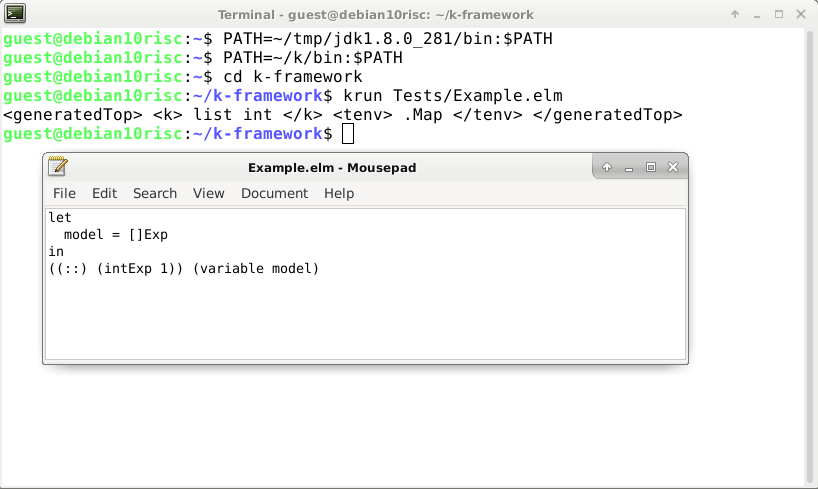
\includegraphics[width=0.75\linewidth]{k} 

}

\caption{The end result}\label{fig:k}
\end{figure}

\section{Refinement Types in Elm}\label{refinement-types-in-elm}

We will now turn to the implementation of the core of the type inference
algorithm discussed in Section \ref{formulating-smt-statements}.

In particular, we will present the \texttt{split}, \texttt{solve} and
\texttt{weaken} functions for computing the strongest refinements for a
set of given subtyping conditions.

We have implemented these functions in Elm itself; to simplify testing,
we have equipped the implementation with a GUI by using an Em package
written by the author called Elm-Action \cite{elmAction} (see Figure
\ref{fig:gui}).

\begin{figure}

{\centering 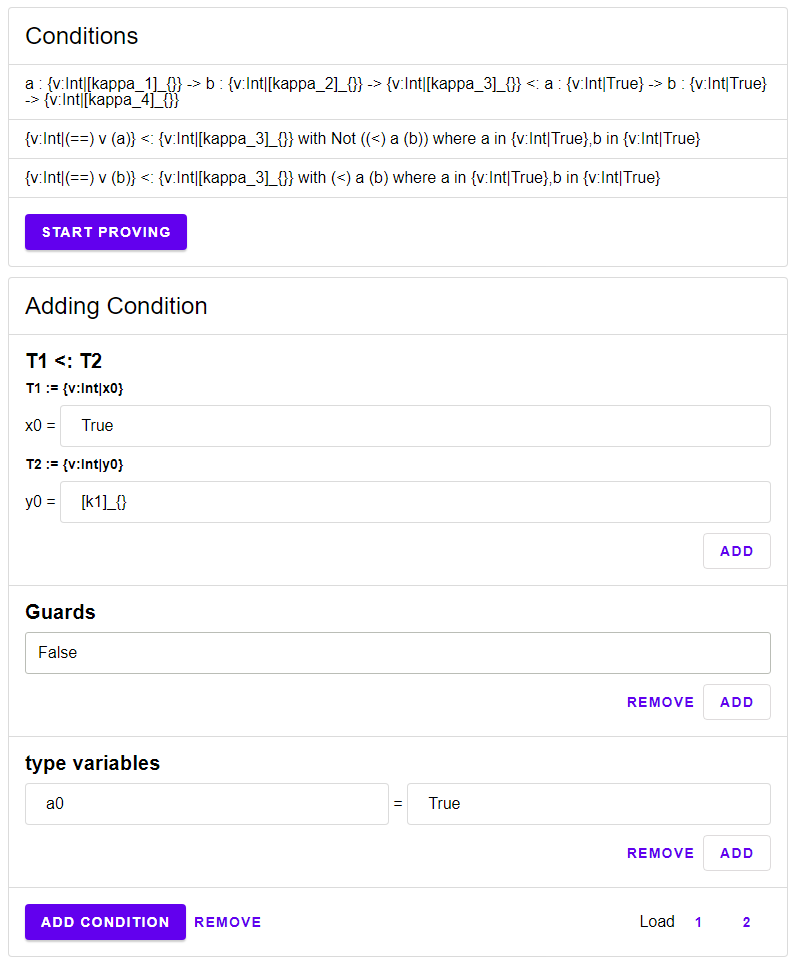
\includegraphics[width=0.75\linewidth]{ui} 

}

\caption{A GUI for writing a set of input conditions.}\label{fig:gui}
\end{figure}

The architecture of a typical elm program is similar to that of a state
machine: First a \texttt{init} function is called to define the initial
state (in Elm typically called \texttt{Model}). The state is then passed
to the \texttt{view} function that displays the state as an HTML
document on the screen. The user can now interact with the elements on
screen (like pressing a button). Once the user has performed an
interaction, a message describing the action will be passed to an
\texttt{update} function, updating the current state (and with that also
the HTML document on screen).

Our implementation consists of three different programs called
\texttt{Setup}, \texttt{Assistant} and \texttt{Done}. The \texttt{Setup}
program as seen in Figure \ref{fig:gui} handles the creation of our
conditions. The \texttt{Assistant} program as seen in Figure
\ref{fig:assistant} applies the \texttt{split}, \texttt{solve} and
\texttt{weaken} functions to the conditions. The \texttt{Done} program
as seen in Figure \ref{fig:done} shows the solution.

\begin{figure}

{\centering 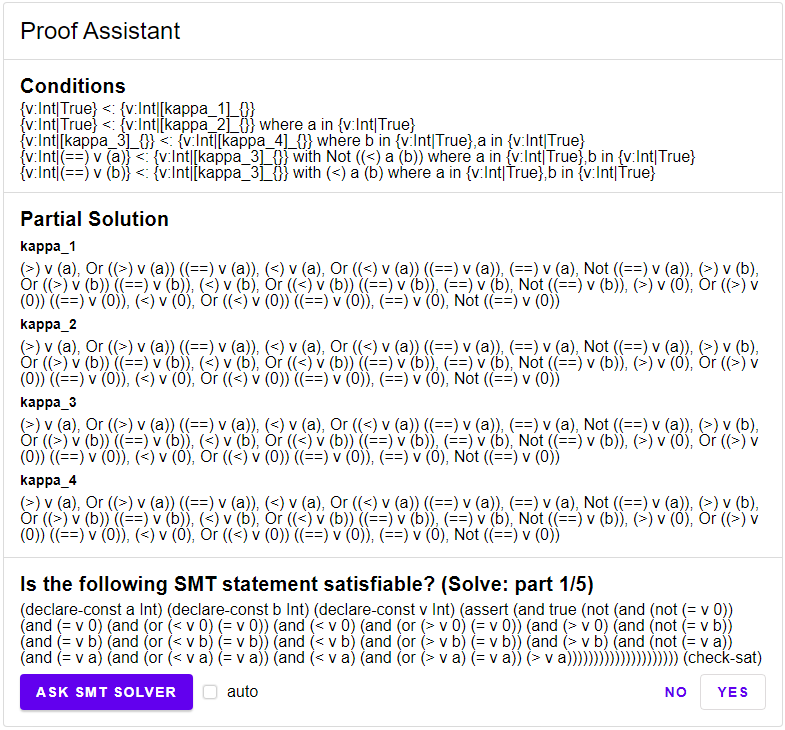
\includegraphics[width=0.75\linewidth]{assistant} 

}

\caption{Proof assistant displaying the current SMT statement}\label{fig:assistant}
\end{figure}

\begin{figure}

{\centering 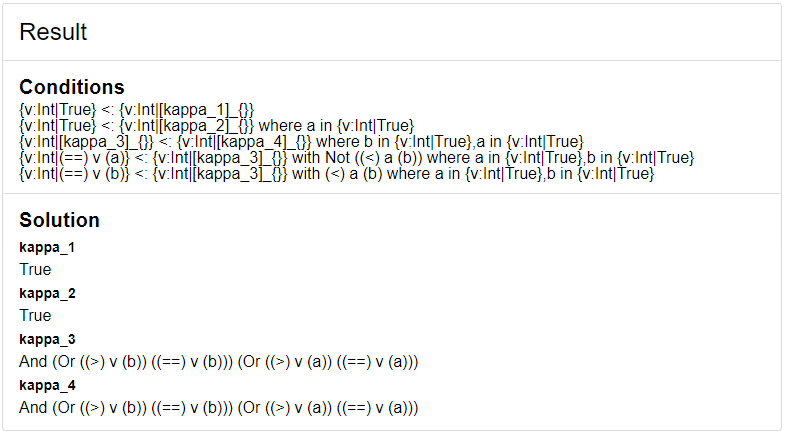
\includegraphics[width=0.75\linewidth]{done} 

}

\caption{The end result}\label{fig:done}
\end{figure}

Our library Elm-Action simplifies the wiring to combine multiple Elm
programs into one. To do so, the library models the different Elm
programs as different states of a meta-level state machine: Each state
is its own state machine. To transition from one program into another we
define a transition function that takes some transition data as an input
and returns the initial state of the new elm program.

We will only discuss the \texttt{Assistant} program, as it is the most
interesting. In this program our state describes a satisfiability
problem. This SAT problem needs to be solved by either the SMT solver or
a human. We are using the SMT solver called Z3. To talk to Z3, we use a
small JavaScript code that communicates between Z3 and Elm. Elm will
send the problem in question through JavaScript to Z3 and then awaits a
response. Once the response has been received, it will then be sent to
the \texttt{update} function, resulting in a new satisfiability problem.
This new problem can be again sent to either Z3 or displayed on the
screen. If this process stops, then the program ends and transitions
into the \texttt{Done} program.

\section{Details of the Elm
Implementation}\label{details-of-the-elm-implementation}

We will now go over the Elm code in more detail.

\subsection{Types}\label{types}

For Liquid Types we use the following representation:

\begin{verbatim}
type alias LiquidType a b =
    ( List
        { name : String
        , type : a
        }
    , b
    )
\end{verbatim}

A function
\(a:\{\mathit{Int}\ |\ r1\}\to b:\{\mathit{Int}\ |\ r2\}\to\{\mathit{Int}\ |\ r3\}\)
would be represented as
\texttt{({[}\{name=a,refinement=r1\},\{name=b,refinement=r2\}{]},r3)}.
We allow different types for \texttt{a} and \texttt{b}:

\begin{verbatim}
type SimpleLiquidType
    = IntType Refinement
    | LiquidTypeVariable Template
\end{verbatim}

Possible types for \texttt{a} and \texttt{b} are either the most general
\texttt{SimpleLiquidType} or the more specific types \texttt{Refinement}
and \texttt{Template}. Note on the naming: \texttt{SimpleLiquidType} is
\enquote{simple} in the sense that it is not a function type.

In respect to conditions we have two types:

\begin{verbatim}
type alias Condition =
    { smaller : LiquidType Template SimpleLiquidType
    , bigger : LiquidType Refinement Template
    , guards : List Refinement
    , typeVariables : List ( String, Refinement )
    }


type alias SimpleCondition =
    { smaller : SimpleLiquidType
    , bigger : Template
    , guards : List Refinement
    , typeVariables : List ( String, Refinement )
    }
\end{verbatim}

\texttt{SimpleCondition} is the implementation of \(\mathcal{C}^-\).

\subsection{Transition}\label{transition}

The \texttt{Assistant} program starts by obtaining some transition data
from the \texttt{Setup} program. This transition data will then be used
to initiate the state.

\begin{verbatim}
type alias Transition =
    List SimpleCondition
\end{verbatim}

We obtain simple conditions from the \emph{Split} function. This is a
one-to-one implementation of the \emph{Split} function previously
described. We will now go through its definition.

\text{\textemdash}

\begin{verbatim}
split : Condition -> Result () (List SimpleCondition)
split =
  let
    rec : Int -> Condition -> Result () (List SimpleCondition)
    rec offset condition =
      case ( condition.smaller, condition.bigger ) of
        ( ( q1 :: t2, t2end ), ( q3 :: t4, t4end ) ) ->
          if q1.name == q3.name then
            rec (offset + 1)
              { condition
              | smaller = ( t2, t2end )
              , bigger = ( t4, t4end )
              , typeVariables =
                ( q3.name, q3.refinement )
                  :: condition.typeVariables
              }
              |> Result.map
                ((::)
                  { smaller = IntType q3.refinement
                  , bigger = q1.refinement
                  , guards = condition.guards
                  , typeVariables = condition.typeVariables
                  }
                )

          else
            Err ()
\end{verbatim}

This first case is equivalent to the following.

\[
\begin{aligned}
&\text{Split}(a:\{\nu:\mathit{Int}\ |\ q_1\}\to \hat{T}_2<:_{\Theta,\Lambda}a:\{\nu:\mathit{Int}\ |\ q_3\}\to\hat{T}_4 )=\\
&\quad\quad\{\{\nu:\mathit{Int}\ |\ q_3\} <:_{\Theta,\Lambda}\{\nu:\mathit{Int}\ |\ q_1\}\}\cup\text{Split}(\hat{T}_2 <:_{\Theta\cup\{(a,q_3)\},\Lambda}\hat{T}_4\})
\end{aligned}
\]

\text{\textemdash}

\begin{verbatim}
        ( ( [], q1 ), ( [], q2 ) ) ->
          [ { smaller = q1
            , bigger = q2
            , guards = condition.guards
            , typeVariables = condition.typeVariables
            }
          ]
            |> Ok
\end{verbatim}

The second case is a direct transformation from a \texttt{Condition}
into a \texttt{SimpleCondition}. For our formal definition of the second
case, this is equivalent to the identity.

\[
\begin{aligned}
&\text{Split}(\{\nu:\mathit{Int}\ |\ q_1\}<:_{\Theta,\Lambda}\{\nu:\mathit{Int}\ |\ q_2\} )=\\
&\quad\quad\{ \{\nu:\mathit{Int}\ |\ q_1\}<:_{\Theta,\Lambda}\{\nu:\mathit{Int}\ |\ q_2\} \}
\end{aligned}
\]

\text{\textemdash}

\begin{verbatim}
        _ ->
          Err ()
  in
  rec 0
\end{verbatim}

The \emph{Split} function is a partial function, therefore we will
return an error if neither case could be applied. If so, the
\texttt{Setup} program will throw an error and the user would need to
correct the given conditions. For a valid condition, the \emph{Split}
function will always be successful. Once successful the new list of
\texttt{SimpleCondition}s will be passed as transition data to the
\texttt{Assistant} program.

\begin{verbatim}
case model.conditions |> List.map Function.split |> Result.combine of
    Ok conds ->
        conds |> List.concat |> Action.transitioning
    Err () ->
        ...
\end{verbatim}

\subsection{Init}\label{init}

After we have split the conditions, we initiate the Elm program. Note
that this program will be implementing the \emph{Solve} and
\emph{Weaken} functions.

\begin{verbatim}
init : Transition -> ( Model, Cmd Msg )
init conditions =
    let
        initList =
            (conditions
                |> List.map
                    (\{ typeVariables } ->
                        typeVariables
                            |> List.map (\( name, _ ) -> name)
                    )
                |> List.concat
            )
                |> Refinement.init
    in
    ( { conditions = conditions |> Array.fromList
      , predicates =
            conditions
                |> List.concatMap Condition.liquidTypeVariables
                |> List.map (\v -> ( v, initList |> Array.fromList ))
                |> Dict.fromList
      , index = 0
      , weaken = Nothing
      , auto = False
      , error = Nothing
      }
    , Cmd.none
    )
\end{verbatim}

We now go through all fields of our model.

\begin{itemize}
\tightlist
\item
  \texttt{conditions} contains a copy of the conditions.
\item
  \texttt{predicates} contains a dictionary, mapping every liquid type
  variable to the initial set of predicates \(\mathit{Init}(V)\).
  (Equivalent to \texttt{Refinement.init})
\item
  \texttt{index} contains the index of the current condition. Keep in
  mind, that the loop from the \emph{Solve} function is actually
  modelled as state transitions. Therefore, we can assume that we are
  always investigating one specific condition at a time. If not, then
  the program would have already stopped.
\item
  \texttt{weaken} says if we are currently weakening a condition. If
  this is set to \texttt{Nothing} then we are in the \emph{Solve}
  function, else its \texttt{Just\ i} where \texttt{i} is the index of
  the predicate that we are currently investigating.
\item
  \texttt{auto} is a boolean expression that says if the SMT solver
  should be asked directly. If set to \texttt{False}, then the user may
  decide the satisfiability of the current SMT statement.
\item
  \texttt{error} contains any error message that should be displayed to
  the user. These errors come directly from the SMT solver.
\end{itemize}

\subsection{Update}\label{update}

\begin{verbatim}
update : (String -> Cmd msg) -> Msg -> Model -> Update msg
update sendMsg msg model =
    case msg of
        GotResponse bool ->
            handleResponse sendMsg bool { model | error = Nothing }
        ...

handleResponse : (String -> Cmd msg) -> Bool -> Model -> Update msg
handleResponse sendMsg bool model =
    case model.weaken of
        Just weaken ->
            handleWeaken weaken sendMsg bool model

        Nothing ->
            handleSolve sendMsg bool model
\end{verbatim}

We have stored the additional information needed for the \emph{Weaken}
function in \texttt{model.weaken}. We therefore check the content of
\texttt{model.weaken}. We check the content of \texttt{model.weaken}, If
it is \texttt{Nothing} we know that we are in the \emph{Solve} function,
else we know that we are currently in the \emph{Weaken} function.

\subsubsection{The Solve Function}\label{the-solve-function}

\begin{verbatim}
handleSolve : (String -> Cmd msg) -> Bool -> Model -> Update msg
handleSolve sendMsg bool model =
    if bool then
        --Start weaking
        case
            model.conditions
                |> Array.get model.index
        of
            Just { bigger } ->
                { model
                    | weaken =
                        Just
                            { index = 0
                            , liquidTypeVariable = 
                                bigger |> Tuple.first
                            }
                }
                    |> handleAuto sendMsg

            Nothing ->
                Action.updating ( model, Cmd.none )
\end{verbatim}

If the incoming result is \texttt{True} it means that the SMT statement
is satisfiable. Therefore, we start the \emph{Weaken} function. To do
so, we initiate the weakening index at \texttt{0} and also store the
liquid type variable whose corresponding refinement we want to weaken.

\text{\textemdash}

\begin{verbatim}
    else
        --Continue
        let
            index =
                model.index + 1
        in
        if index >= (model.conditions |> Array.length) then
            Action.transitioning
                { conditions = model.conditions
                , predicates =
                    model.predicates
                        |> Dict.map 
                          (\_ -> Array.toList >> Refinement.conjunction)
                }

        else
            { model
                | index = index
            }
                |> handleAuto sendMsg
\end{verbatim}

If the incoming result is \texttt{False}, then we check out the next
condition. If there exists no following condition, then the function is
done. We end the Elm program by transitioning into the \texttt{Done}
program.

\subsubsection{The Weaken Function}\label{the-weaken-function}

\begin{verbatim}
handleWeaken :
    { index : Int
    , liquidTypeVariable : Int
    }
    -> (String -> Cmd msg)
    -> Bool
    -> Model
    -> Update msg
handleWeaken weaken sendMsg bool model =
    if bool then
        --Remove
        let
            predicates =
                model.predicates
                    |> Dict.update weaken.liquidTypeVariable
                        (Maybe.map
                            (Array.removeAt weaken.index)
                        )
        in
        if
            weaken.index
                >= (predicates
                        |> Dict.get weaken.liquidTypeVariable
                        |> Maybe.map Array.length
                        |> Maybe.withDefault 0
                   )
        then
            { model
                | predicates = predicates
                , weaken = Nothing
                , index = 0
            }
                |> handleAuto sendMsg

        else
            { model
                | predicates = predicates
            }
                |> handleAuto sendMsg
\end{verbatim}

If the incoming result is \texttt{False}, then the SMT statement is
unsatifiable. Thus, we remove the predicate. If no predicate exists, we
finish the \emph{Weaken} function by setting \texttt{model.weaken} to
\texttt{Nothing}.

\text{\textemdash}

\begin{verbatim}
    else
        --Continue
        let
            index =
                weaken.index + 1
        in
        if
            index
                >= (model.predicates
                        |> Dict.get weaken.liquidTypeVariable
                        |> Maybe.map Array.length
                        |> Maybe.withDefault 0
                   )
        then
            { model
                | weaken = Nothing
                , index = 0
            }
                |> handleAuto sendMsg

        else
            { model
                | weaken =
                    Just
                        { liquidTypeVariable = weaken.liquidTypeVariable
                        , index = index
                        }
            }
                |> handleAuto sendMsg
\end{verbatim}

If the incoming result is \texttt{True}, then the SMT statement is
satisfiable. We therefore check out the next predicate. We finish the
function if no following predicate exists. To do so we again set
\texttt{model.weaken} to \texttt{Nothing}.

\subsection{The SMT Statement}\label{the-smt-statement}

After every update we check if the SMT statement should be automatically
sent to the SMT solver.

\begin{verbatim}
handleAuto : (String -> Cmd msg) -> Model -> Update msg
handleAuto sendMsg model =
    if model.auto then
        ( model
        , model
            |> smtStatement
            |> Maybe.map sendMsg
            |> Maybe.withDefault Cmd.none
        )
            |> Action.updating

    else
        Action.updating
            ( model, Cmd.none )
\end{verbatim}

If not, it will be displayed on the screen. Either way we need to
compute the SMT statement for the given model.

\begin{verbatim}
smtStatement : Model -> Maybe String
smtStatement model =
    let
        toString : SimpleCondition -> String
        toString condition =
            case model.weaken of
                Just weaken ->
                    statementForWeaken weaken model condition

                Nothing ->
                    statementForSolve model condition
    in
    model.conditions
        |> Array.get model.index
        |> Maybe.map toString
\end{verbatim}

The statement differes between the \emph{Solve} and the \emph{Weaken}
function.

\subsubsection{The SMT Statement for
Solve}\label{the-smt-statement-for-solve}

For the \emph{Solve} function we translate the condition directly into
the SMT statement.

\begin{verbatim}
statementForSolve : Model -> SimpleCondition -> String
statementForSolve model condition =
    condition
        |> Condition.toSMTStatement
            (model.predicates
                |> Dict.map (\_ -> Array.toList 
                  >> Refinement.conjunction)
            )
\end{verbatim}

The actual translation happens in \texttt{Condition.toSMTStatement}. The
translation is taken directly from the described \emph{Solve} function.
We therefore will now compare both with another.

\text{\textemdash}

\begin{verbatim}
toSMTStatement : Dict Int Refinement -> SimpleCondition -> String
toSMTStatement dict { smaller, bigger, guards, typeVariables } =
    let
        typeVariablesRefinements : List Refinement
        typeVariablesRefinements =
            typeVariables
                |> List.map
                    (\( b, r ) ->
                        r |> Refinement.rename 
                            { find = "v"
                            , replaceWith = b
                            }
                    )
\end{verbatim}

This is equivalent to the following.

\[
\begin{aligned}
&\text{Let}\\
&\begin{aligned}
  \Theta':= \{\ (&a,r)\\
   | \ &r \text{ has the form } q \land (a,q)\in\Theta \land q\in\mathcal{Q}\\
  \lor \ &r \text{ has the form } [[k]_S]_{S_0}\land (a,q)\in\Theta\\
  &\quad\land q \text{ has the form } [k]_{S_0} \land k\in\mathcal{K} \land S_0\in\mathcal{V}\nrightarrow\mathit{IntExp}\}
  \end{aligned}\\
&\{(b_1,r_1'),\dots,(b_n,r_n')\}=\Theta'\\
&\text{in}
\bigwedge_{j=0}^n [r_j']_{\{(\nu,b_j)\}}
\end{aligned}
\]

\text{\textemdash}

\begin{verbatim}
        r1 : Refinement
        r1 =
            case smaller of
                IntType refinement ->
                    refinement

                LiquidTypeVariable ( int, list ) ->
                    list
                        |> List.foldl
                            (\( k, v ) ->
                                Refinement.substitute
                                    { find = k
                                    , replaceWith = v
                                    }
                            )
                            (dict
                                |> Dict.get int
                                |> Maybe.withDefault IsFalse
                            )
\end{verbatim}

Here we have a case distinction between a refinement and a liquid type
variable. We had the same distinction in our original definition of
\(r1\):

\[
r_1 := \begin{cases}\bigwedge [S(k_1)]_{S_1}&\text{if } q_1 \text{ has the form } [k_1]_{S_1} \text{ for } k\in\mathcal{K}\text{ and } S_1\in\mathcal{V}\nrightarrow\mathit{IntExp}\\
q_1& \text{if }q_1\in\mathcal{Q}
\end{cases},\\
\]

\text{\textemdash}

\begin{verbatim}
        r2 : Refinement
        r2 =
            bigger
                |> Tuple.second
                |> List.foldl
                    (\( k, v ) ->
                        Refinement.substitute
                            { find = k
                            , replaceWith = v
                            }
                    )
                    (dict
                        |> Dict.get (bigger |> Tuple.first)
                        |> Maybe.withDefault IsFalse
                    )
\end{verbatim}

Here we see how we apply the lazy substitution (stored in
\texttt{bigger\ \textbar{}\textgreater{}\ Tuple.second}). In the
original definition, we assumed that we know how to apply a substitution
on the term level:

\[
r_2 := \bigwedge [S(\kappa_2)]_{S_2}
\]

\text{\textemdash}

\begin{verbatim}
        statement : Refinement
        statement =
            (r1
                :: typeVariablesRefinements
                ++ guards
            )
                |> List.foldl AndAlso (IsNot r2)
    in
    (statement
        |> Refinement.variables
        |> Set.toList
        |> List.map (\k -> "(declare-const " ++ k ++ " Int)\n")
        |> String.concat
    )
        ++ ("(assert " 
               ++ (statement |> Refinement.toSMTStatement) 
               ++ ")\n(check-sat)"
           )
\end{verbatim}

The final statement is therefore

\[((\bigwedge_{j=0}^n [r_j']_{\{(\nu,b_j)\}})\land r_1\land p)\land \neg r_2\]
with free variables \(\nu\in\mathbb{Z}\) and \(b_i\in\mathbb{Z}\) for
\(i\in\mathbb{N}_1^n\).

\subsubsection{The SMT Statement for
Weaken}\label{the-smt-statement-for-weaken}

For the \emph{Weaken} function we modify the statement.

\begin{verbatim}
statementForWeaken :
    { index : Int, liquidTypeVariable : Int }
    -> Model
    -> SimpleCondition
    -> String
statementForWeaken weaken model condition =
  condition
    |> Condition.toSMTStatement
      (model.predicates
        |> Dict.map (\_ -> Array.toList >> Refinement.conjunction)
        |> Dict.update (condition.bigger |> Tuple.first)
          (Maybe.map
            (\_ ->
              model
                |> getLazySubstitute
                |> List.foldl
                  (\( find, replaceWith ) ->
                    Refinement.substitute
                      { find = find
                      , replaceWith = replaceWith
                      }
                  )
                  (model.predicates
                    |> Dict.get (condition.bigger |> Tuple.first)
                    |> Maybe.andThen (Array.get weaken.index)
                    |> Maybe.withDefault IsFalse
                  )
            )
          )
      )
\end{verbatim}

We replace the value at the point
\texttt{condition.bigger\ \textbar{}\textgreater{}\ Tuple.first} with
the predicate in question. The same happens in our formal definition.
The resulting SMT statement for the predicate \(q\) is therefore

\[((\bigwedge_{j=0}^n [r_j']_{\{(\nu,b_j)\}})\land r_1\land p)\land \neg q\]
with free variables \(\nu\in\mathbb{Z}\) and \(b_i\in\mathbb{Z}\) for
\(i\in\mathbb{N}_1^n\).

We therefore swap the result around: We keep the predicate if we SMT
statement is unsatifiable. This is equivalent to saying we keep the
predicate if the negated SMT statement is satifiable:

\[\neg((\bigwedge_{j=0}^n [r_j']_{\{(\nu,b_j)\}})\land r_1\land p)\lor q
\] with free variables \(\nu\in\mathbb{Z}\) and \(b_i\in\mathbb{Z}\) for
\(i\in\mathbb{N}_1^n\).

\section{Demonstration}\label{demonstration}

For a demonstration, we will consider the following function.

\begin{verbatim}
max : a:{ v:Int|True } -> b:{ v:Int|True } -> { v:Int|k4 };
max =
  \a -> \b ->
    if 
      (<) a b
    then
      b
    else
      a
\end{verbatim}

To check the validity of the type signature, we will first infer the
type of the function and then compare it with the type signature. Using
the inference rule, we obtain as a result the type

\[
\{v:\mathit{Int}\ |\ \kappa_1\} \to \{v:\mathit{Int}\ |\ \kappa_2\} \to \{v:\mathit{Int}\ |\ \kappa_3\}
\]

with the following conditions.

\[
\begin{aligned}
\{\nu:\mathit{Int}\ |\ \nu = b\}&<:_{\{(a,\{\mathit{Int}\ |\ \mathit{True}\}),(b,\{\mathit{Int}\ |\ \mathit{True}\})\},\{a < b\}}\{\nu:\mathit{Int}\ |\ \kappa_3\},\\
  \{\nu:\mathit{Int}\ |\ \nu = a\}&<:_{\{(a,\{\mathit{Int}\ |\ \mathit{True}\}),(b,\{\mathit{Int}\ |\ \mathit{True}\})\},\{\neg (a < b)\}}\{\nu:\mathit{Int}\ |\ \kappa_3\},
\end{aligned}
\]

We now write the validity check of the type signature as a condition.

\[
\begin{aligned}
  & a:\{\nu:\mathit{Int}\ |\ \kappa_1\}\to b:\{\nu:\mathit{Int}\ |\ \kappa_2\}\to\{\nu:\mathit{Int}\ |\ \kappa_3\}\\
  &\quad<:_{\{\},\{\}}a:\{\nu:\mathit{Int}\ |\ \mathit{True}\}\to b:\{\nu:\mathit{Int}\ |\ \mathit{True}\}\to\{\nu:\mathit{Int}\ |\ \kappa_4\}\\
\end{aligned}
\]

Figure \ref{fig:assistant1} shows how the conditions can be inserted
into the elm program.

\begin{figure}

{\centering 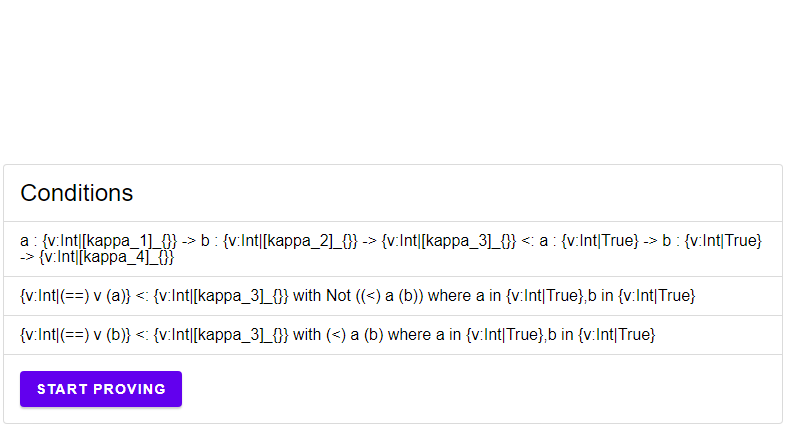
\includegraphics[width=0.75\linewidth]{1} 

}

\caption{The conditions of the max-function}\label{fig:assistant1}
\end{figure}

If we click on the \enquote{Start Proving} button, the
\texttt{Assistant} program will start and get the list of conditions as
the transition data. It now applies the \emph{Split} function to the
conditions and computes the first SMT statement, as seen in Figure
\ref{fig:assistant2}.

\begin{figure}

{\centering 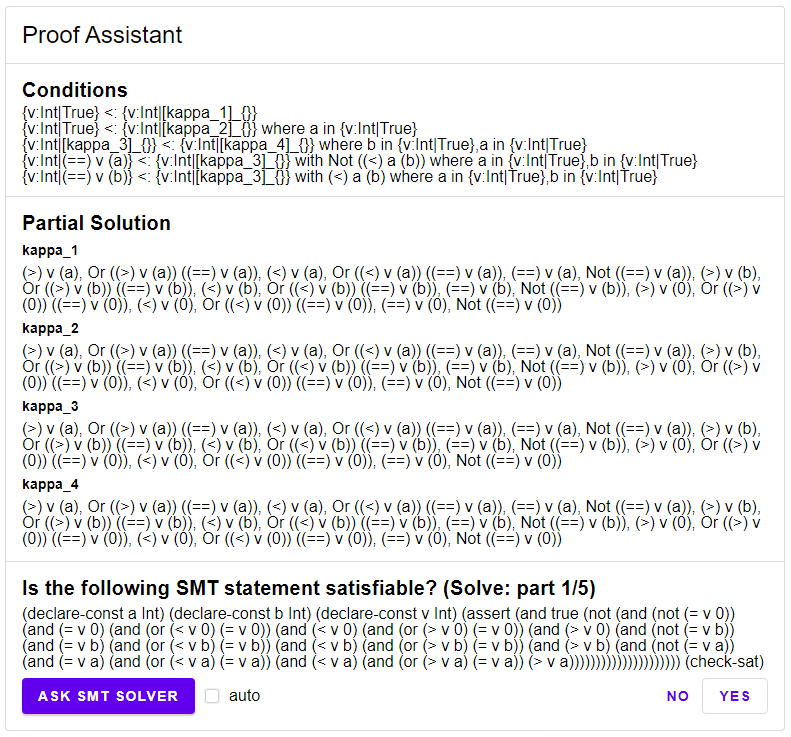
\includegraphics[width=0.75\linewidth]{2} 

}

\caption{The conditions of the max-function}\label{fig:assistant2}
\end{figure}

Here we see the conditions on top, displaying the conditions that are
now split. Next we see that for each \texttt{kappa} the set of
predicated have been initiated with all possible predicates for
variables \texttt{a} and \texttt{b}. Below it presents the first SMT
statement in the \texttt{Solve}-step, mainly if the first condition is
not satisfiable for the current value of \texttt{kappa\_1}. Therefore,
the SMT statement is satisfiable.

Next, the program goes into \emph{Weaken}-mode and starts checking each
and every predicate currently associated with \texttt{kappa\_1}, as seen
in Figure \ref{fig:assistant3}.

\begin{figure}

{\centering 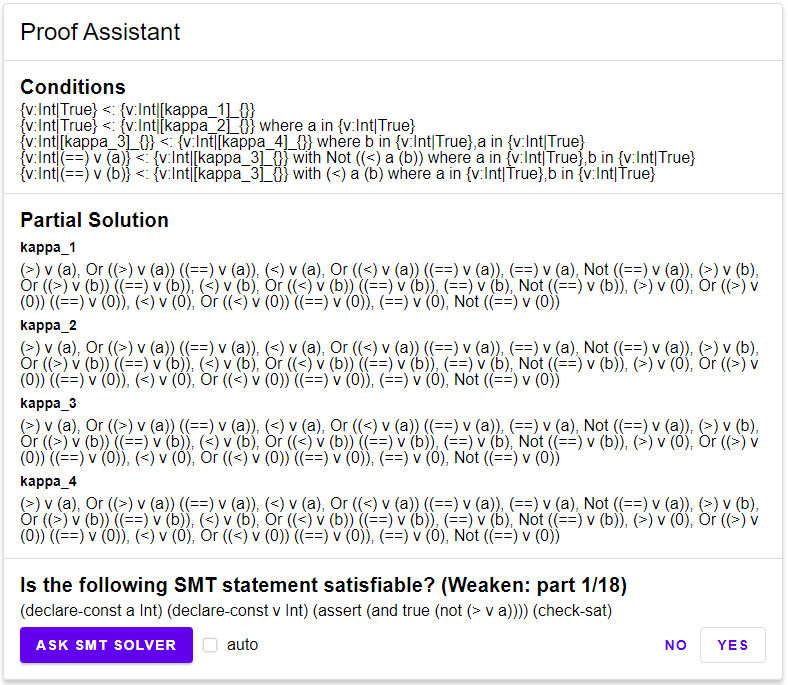
\includegraphics[width=0.75\linewidth]{3} 

}

\caption{Weakening the predicates.}\label{fig:assistant3}
\end{figure}

Once it has checked every predicate, it goes back to \emph{Solve}-mode
and repeats. In Figure \ref{fig:assistant4} one can see the result after
a few iterations.

\begin{figure}

{\centering 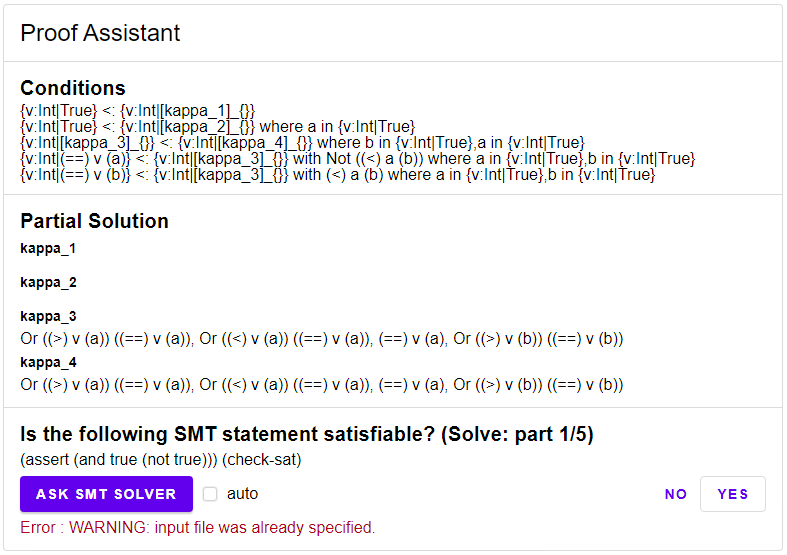
\includegraphics[width=0.75\linewidth]{4} 

}

\caption{The partial result after a few iterations.}\label{fig:assistant4}
\end{figure}

Once every condition is valid (meaning that all SMT statements in the
\emph{Solve}-mode are unsatifiable) the program holds and the result is
displayed as seen in Figure \ref{fig:done}.

\chapter{Conclusions}\label{conclusions}

In this thesis, we have investigated the type system for the Elm
language and discussed its extension by refinement types.

The original intent was to have an implementation of the type checker
for liquid types. We expected that the resulting liquid types are
defined such that non-negative integers, range types and non-zero
integers can be defined. We expected to implement liquid types for
\texttt{Int}, \texttt{Bool} and tuples of liquid types. Additionally, we
expected that the inferred type of the \texttt{max} function can be
sharp. Such a sharp refinement is
\((a \leq \nu) \land (b \leq \nu)\land (\nu = b \lor \nu = a)\).

Indeed, the resulting type system is capable of defining all described
integer types and also allows inferring liquid types for functions over
integers. However, It does not include liquid types over \texttt{Bool}
and tuples. Additionally, the inferred type of the max function is not
sharp: \((a \leq \nu) \land (b \leq \nu)\). Adding these missing
features would have been too time-consuming and would not provide any
new revelations:

\begin{itemize}
\tightlist
\item
  The inclusion of Booleans would have meant that we would have needed
  to type check the liquid expressions. This would have added
  unnecessary complexity, as we are mainly interested in subtypes of
  integers.
\item
  Tuples would have been easy to add but would not yield additional
  behaviour, as Tuples as arguments can be flattened and then
  transformed into a list of arguments and Tuples as a return argument
  are syntax sugar for defining multiple functions with the same input
  values.
\item
  To infer a sharp refinement for the \texttt{max} function, one can
  simply add \(\nu = b \lor \nu = a\) to the search space, but that is
  not very sophisticated. Another way would be to add \(P \lor Q\) for a
  specific set of allowed predicates for \(P\) and \(Q\). We used our
  Elm implementation to quickly test this for the definition of \(P\)
  and \(Q\) not containing \(\lor\). The resulting refinement was sharp
  but included a lot of trivial conditions. The search space increased
  by a factor of four. This factor could be decreased by ensuring that
  no two predicates are equivalent.
\end{itemize}

While working on the thesis it became clear that the original
expectations did not completely match the possibilities of liquid types.
In particular, the expressiveness of liquid types is directly dependent
on the initial set of predicates and the allowed expressions in
\(\mathcal{Q}\). Extending the allowed expressions in \(\mathcal{Q}\)
requires that the SMT solver can still cope with them. In contrast to
our original expectation, the set of predicates \(\mathcal{Q}\) allowed
in if-branches is a superset of the predicates allowed in refinements.
Additionally, the search space for the derived predicates must be
finite. This means that no matter how big the space we are considering
is, there will always be a predicate in \(\mathcal{Q}\) that cannot be
found.

There are multiple future topics that can be explored.

\begin{itemize}
\tightlist
\item
  The set of allowed expressions \(\mathcal{Q}\) and the search space
  for the inferred refinements can be extended to sharpen the inferred
  predicates. At some point, this would also need to include an
  algorithm to simplify the inferred predicates. Otherwise, the inferred
  predicates can only be hardly read by humans.
\item
  The current implementation in Elm can be extended to a full type
  checker by using the Elm-in-Elm compiler \autocite{elmInElm}. This
  would require some changes to the type checker part of the Elm-in-Elm
  compiler. The updated checker would need to collect the subtyping
  conditions while inferring the type (as discussed in Section
  \ref{liquid-types-for-elm}). This can not be done by simply traversing
  the abstract syntax tree. Such an addition would be simple but
  tedious, as every type inference rule would need to be updated.
\item
  One can try to implement a specific type in Elm without liquid types.
  Liquid types make a type system incomplete. Therefore, this is a far
  better solution of implementing a specific type. For the range type,
  the author of this thesis has actually found another way, namely to
  implement these types using phantom types (an algebraic type were not
  all type variables are used) \autocite{elmStaticArray}.
\end{itemize}

Working on this thesis gave insights into the inner workings of liquid
types. It showcased its strengths but also its weaknesses. Liquid types
are an interesting topic but are not really a good fit for the Elm
language and the philosophies behind it. \newpage

\appendix


\chapter{Source Code}\label{source-code}

The source code discussed in this thesis can be found under

\url{https://github.com/orasund/elm-refine}.

\printbibliography


\end{document}
